\section{Optimal MVA cuts to maximize signal significance}

As we already introduced in previous section, we now train the MVA in
a Higgs mass window, which is a roughly fitted Gaussian mean
$\pm$ one sigma. The ten variables used in MVA are almost uncorrelated
and do not sculpt the four body mass distribution. We apply the MVA
output requirement just as a single cut as other cuts we are applying
for this analysis.

We optimized the likelihood on the basis of a scan over a range of MVA
cut values at discrete intervals. The figure of merit was chosen to be
the expected median exclusion limit achieved for the cut value based
on the same limit setup described in AN-12-024, and a reasonable
assumption on the systematics. The results in all cases revealed an
optimum cut value that minimized the expected limit with a resolution
better than a tenth of the signal strength excluded.

The data-MC comparison plots are shown in
Fig.~\ref{fig:mva:plots-mva2j170mu} to~\ref{fig:mva:plots-mva3j600mu}.
Agreement on MVA ouput between data and MC is good in the region of
phase space where the cuts are made. The MVA output for top pair
events in data and MC indicates that the agreement is good at high MVA
values where the Higgs sits.


\clearpage
%%%%%%%%%%%%%%%%%%%%%%%%%%%%%%%%%%%%%%%%%%%%%%%%%%%%%%%%%%%%%%%%%%%%%%%%%%%%
%%%%%%%%%%%%%%%%%%% mva2j170mu
\begin{figure}[!t]
  \centering
  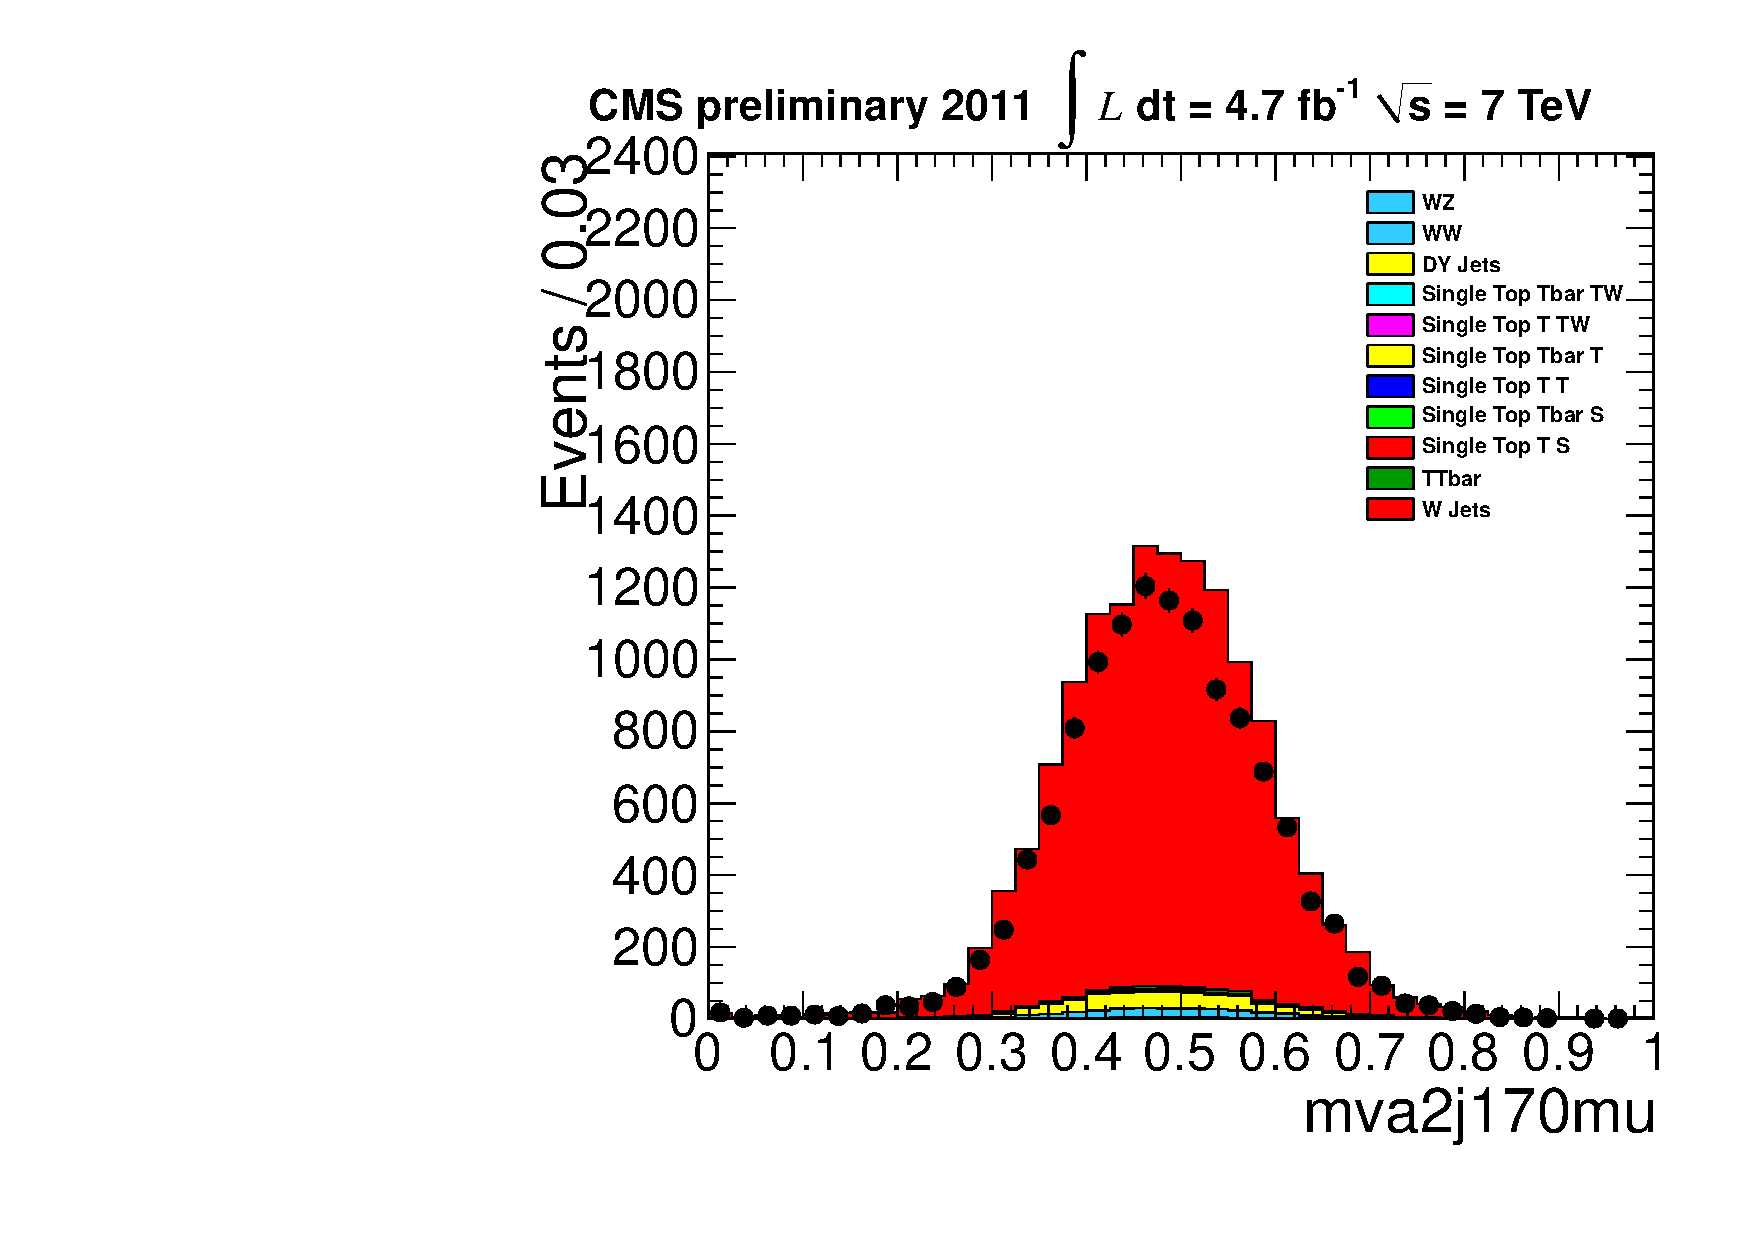
\includegraphics[width=0.49\textwidth]{figs/cl-mva2j170mu-normal.pdf}
  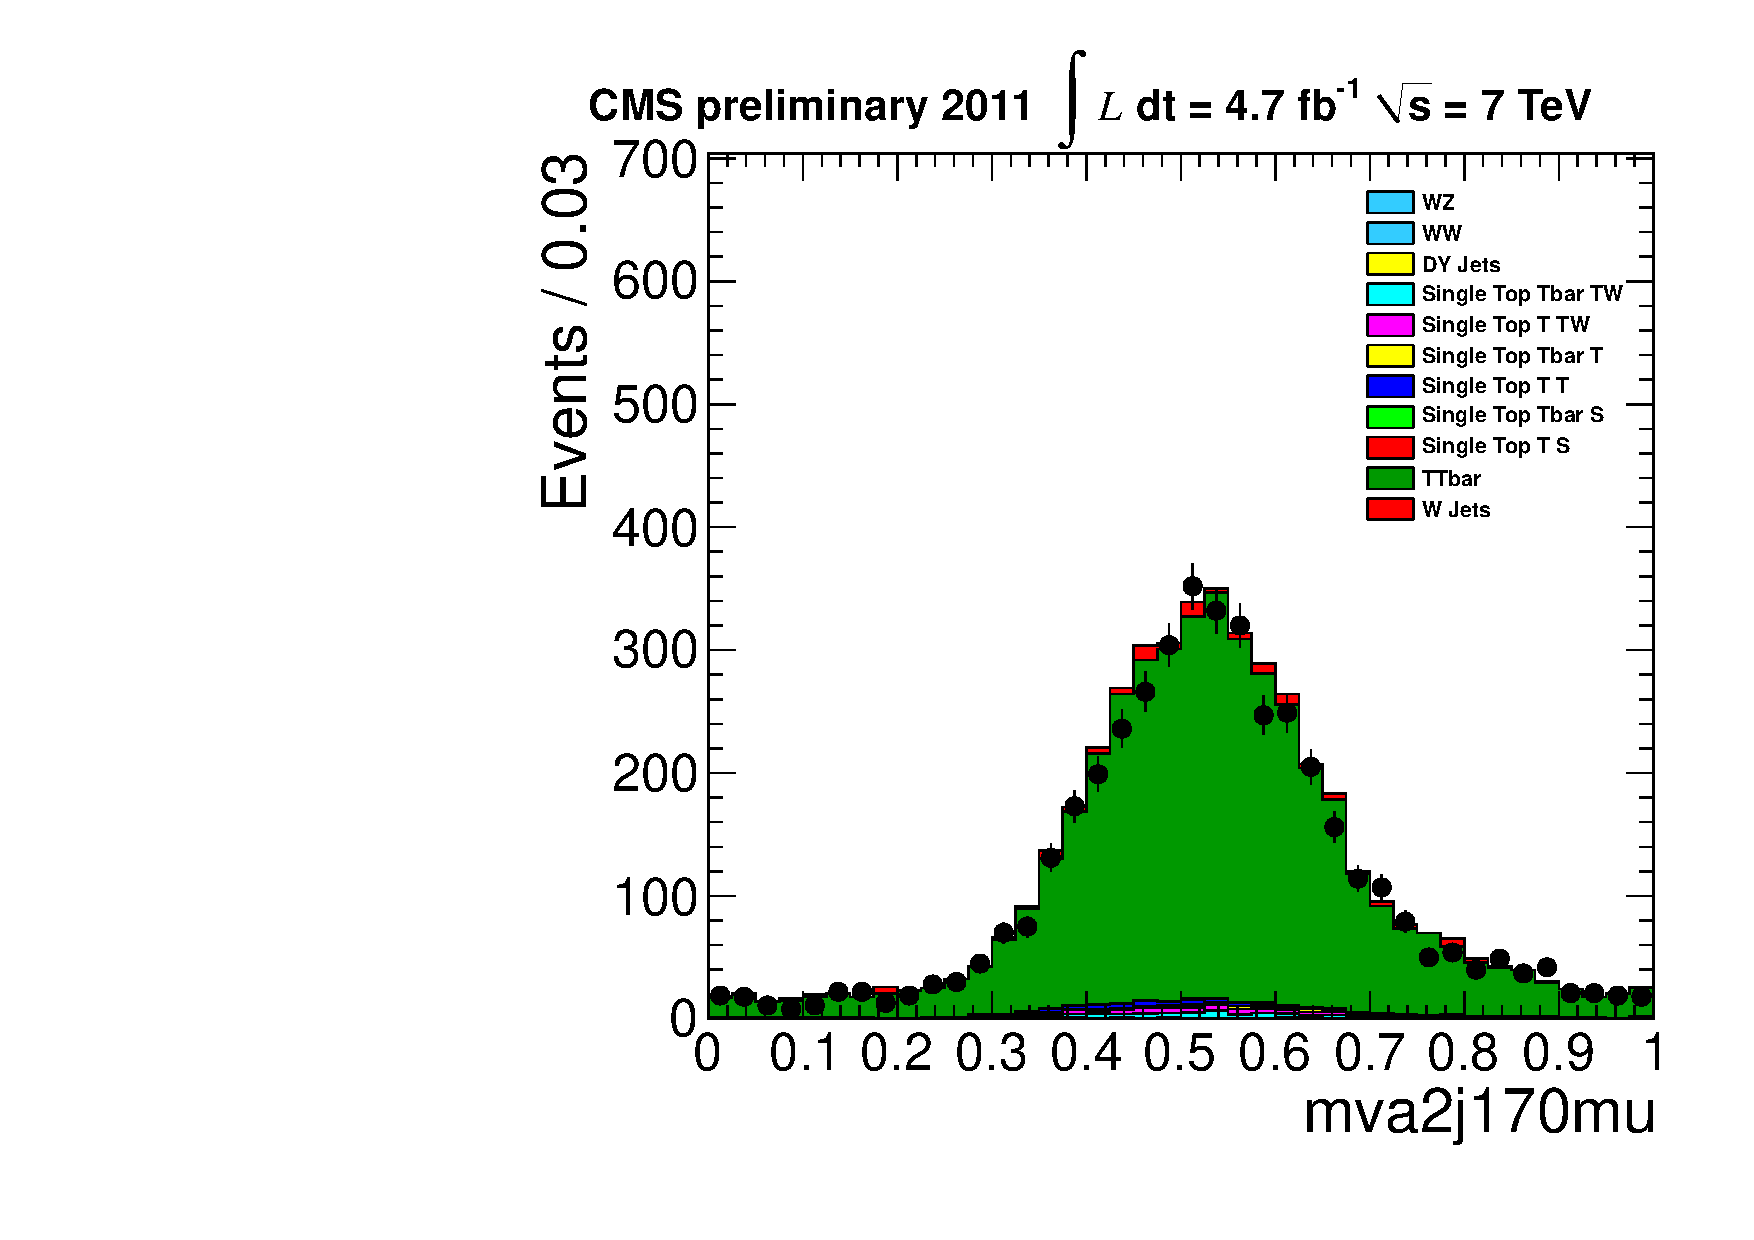
\includegraphics[width=0.49\textwidth]{figs/cl-mva2j170mu-inTTbar.pdf}
  \caption{\label{fig:mva:plots-mva2j170mu} The data-MC comparisons
    after standard event selection (left) and top pair
    selection (right) for the working point: mva2j170mu.}
\end{figure}

%%%%%%%%%%%%%%%%%%% mva2j180mu
\begin{figure}[!t]
  \centering
  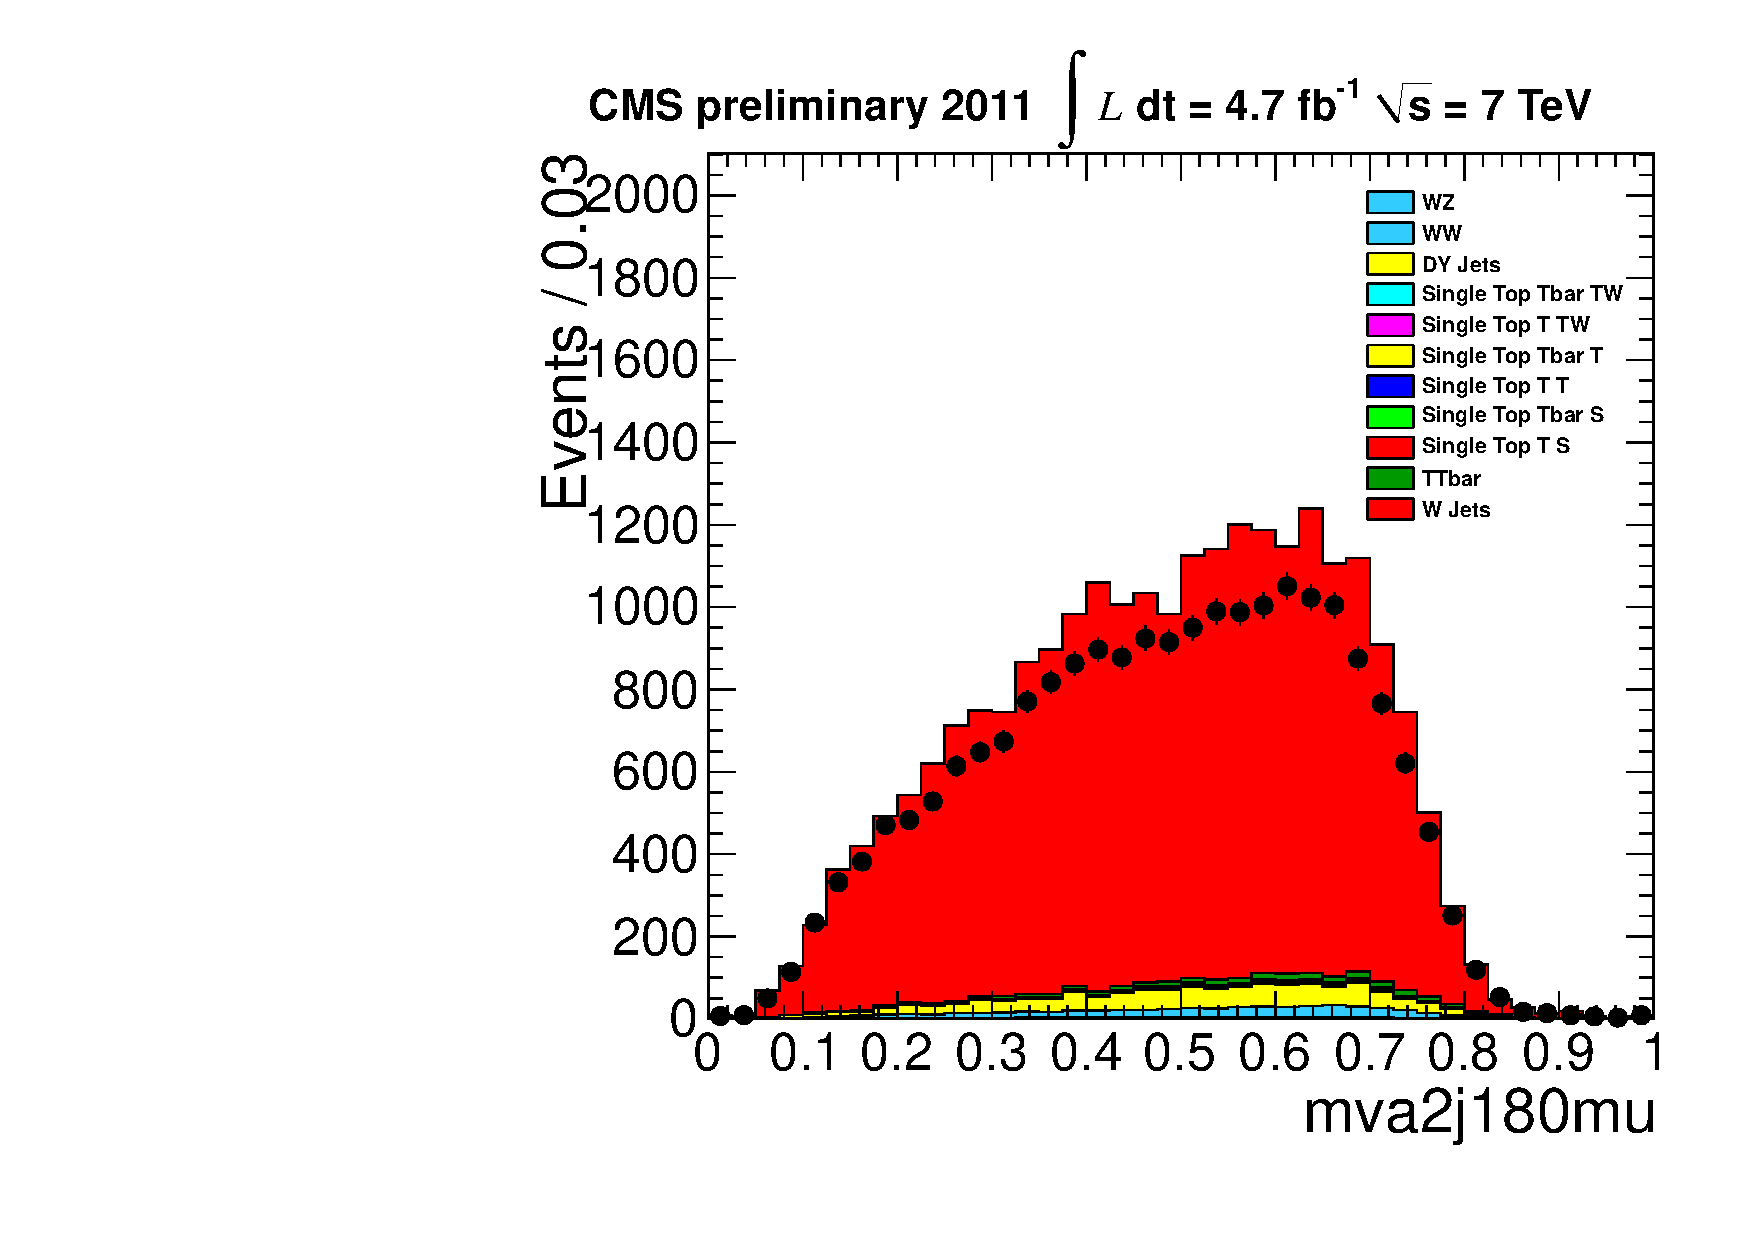
\includegraphics[width=0.49\textwidth]{figs/cl-mva2j180mu-normal.pdf}
  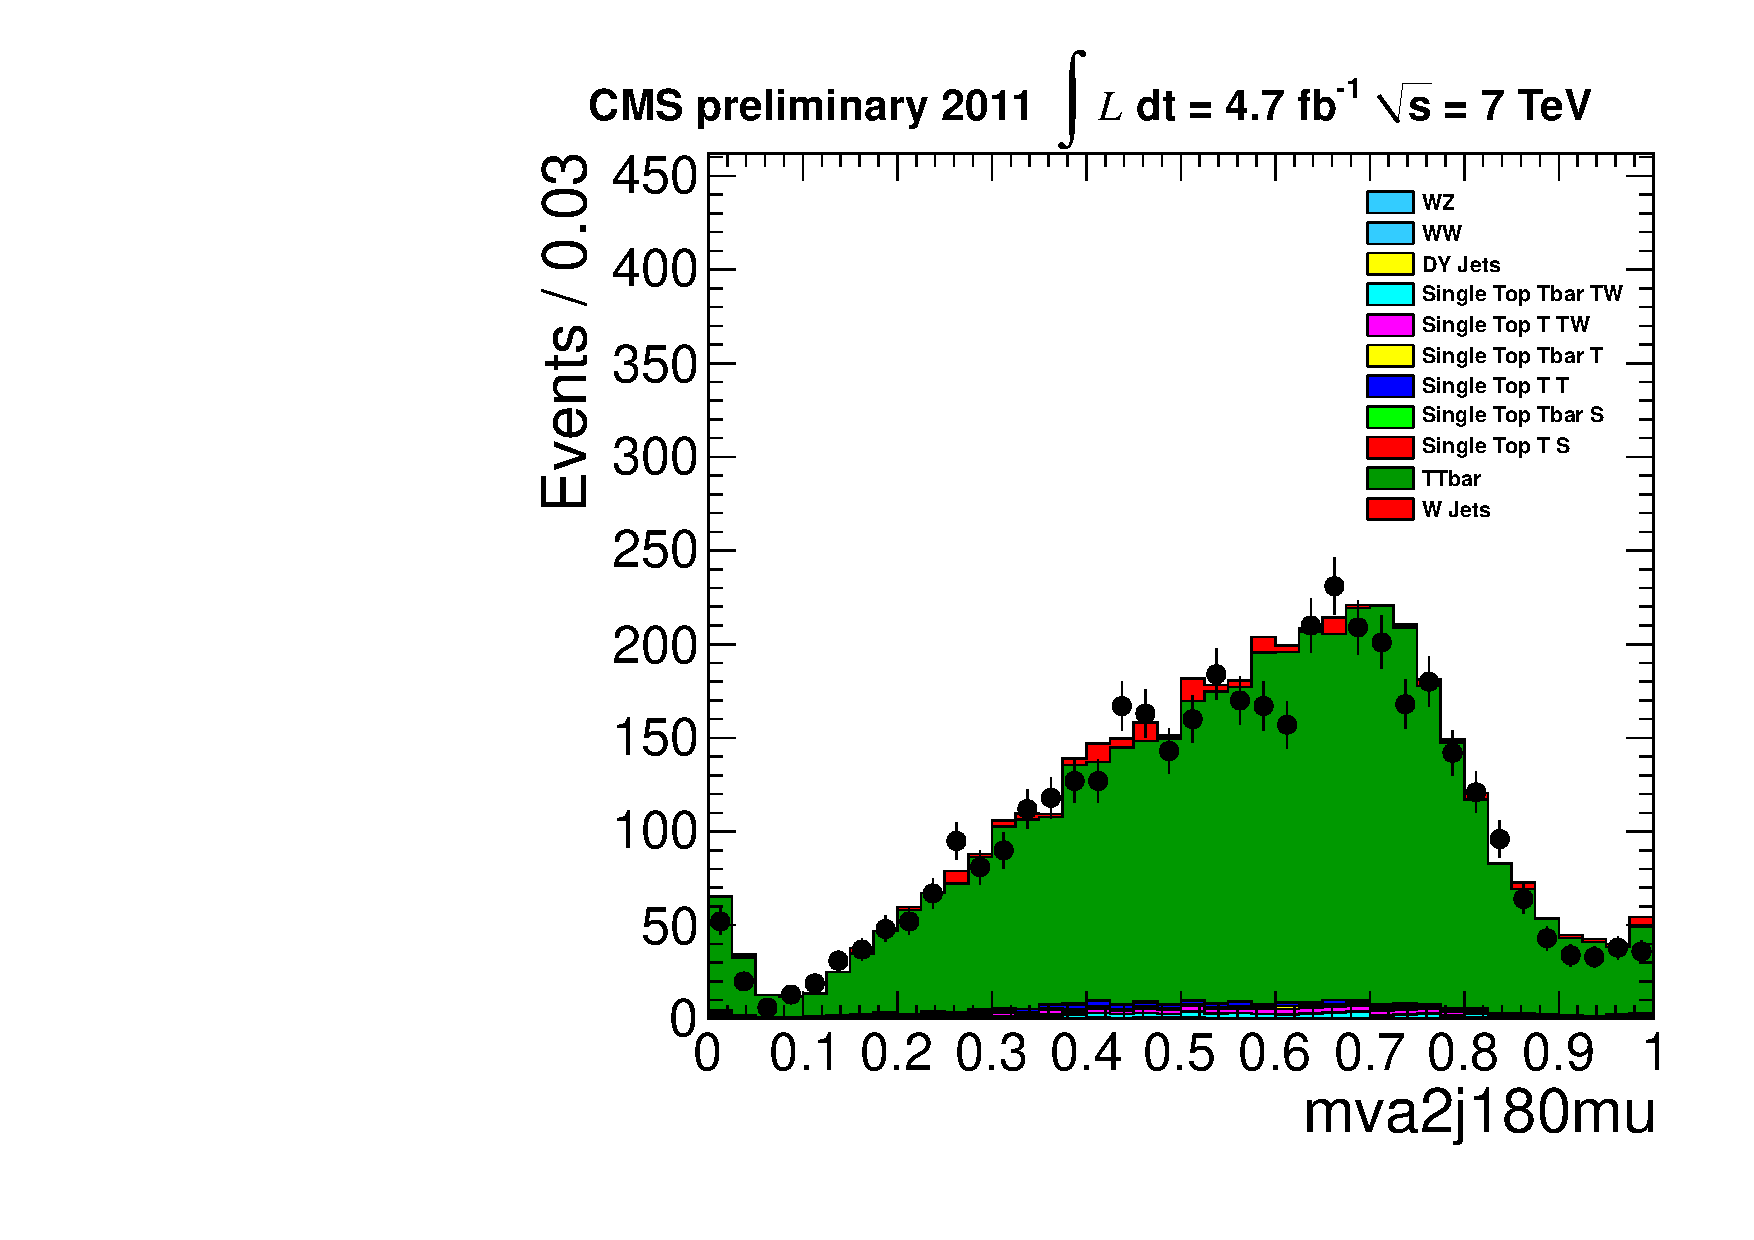
\includegraphics[width=0.49\textwidth]{figs/cl-mva2j180mu-inTTbar.pdf}
  \caption{\label{fig:mva:plots-mva2j180mu} The data-MC comparisons
    after standard event selection (left) and top pair
    selection (right) for the working point: mva2j180mu.}
\end{figure}

%%%%%%%%%%%%%%%%%%% mva2j190mu
\begin{figure}[!t]
  \centering
  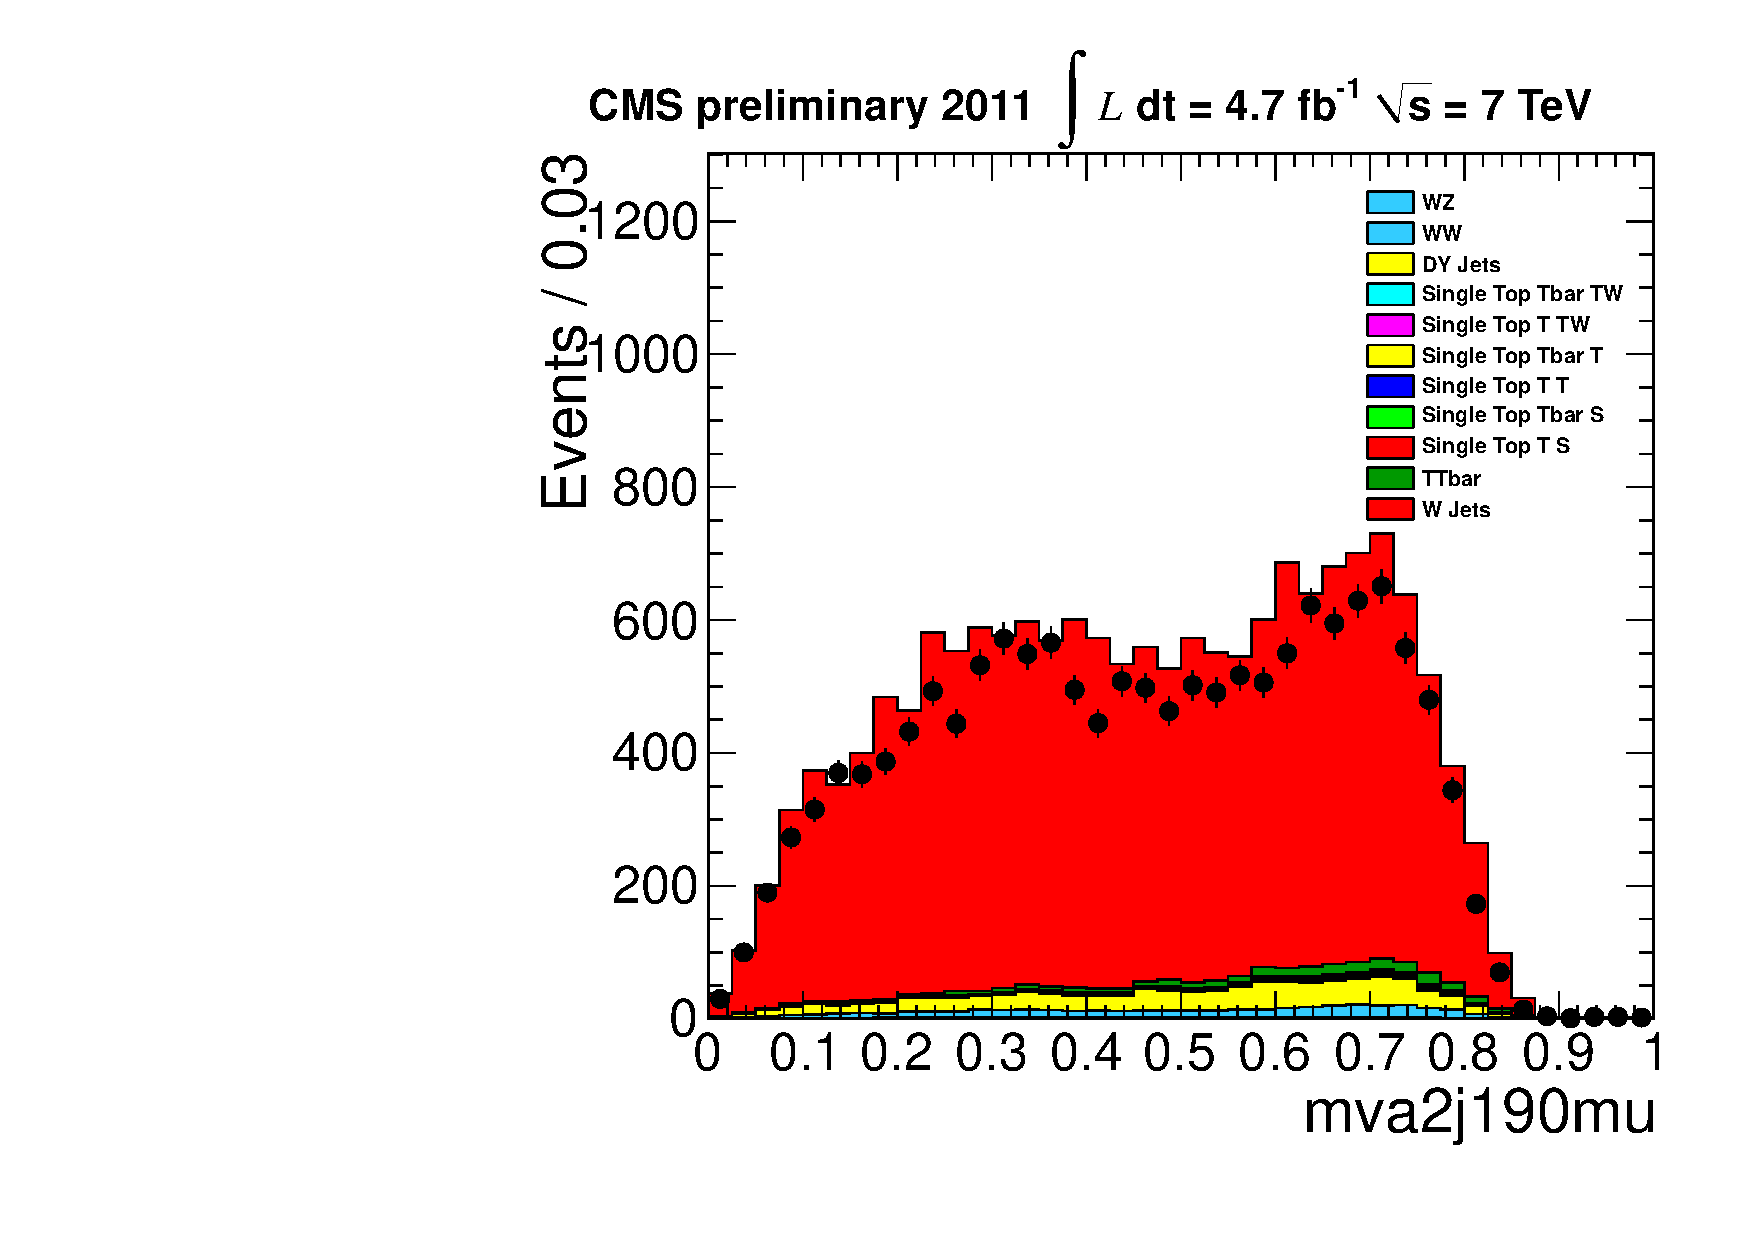
\includegraphics[width=0.49\textwidth]{figs/cl-mva2j190mu-normal.pdf}
  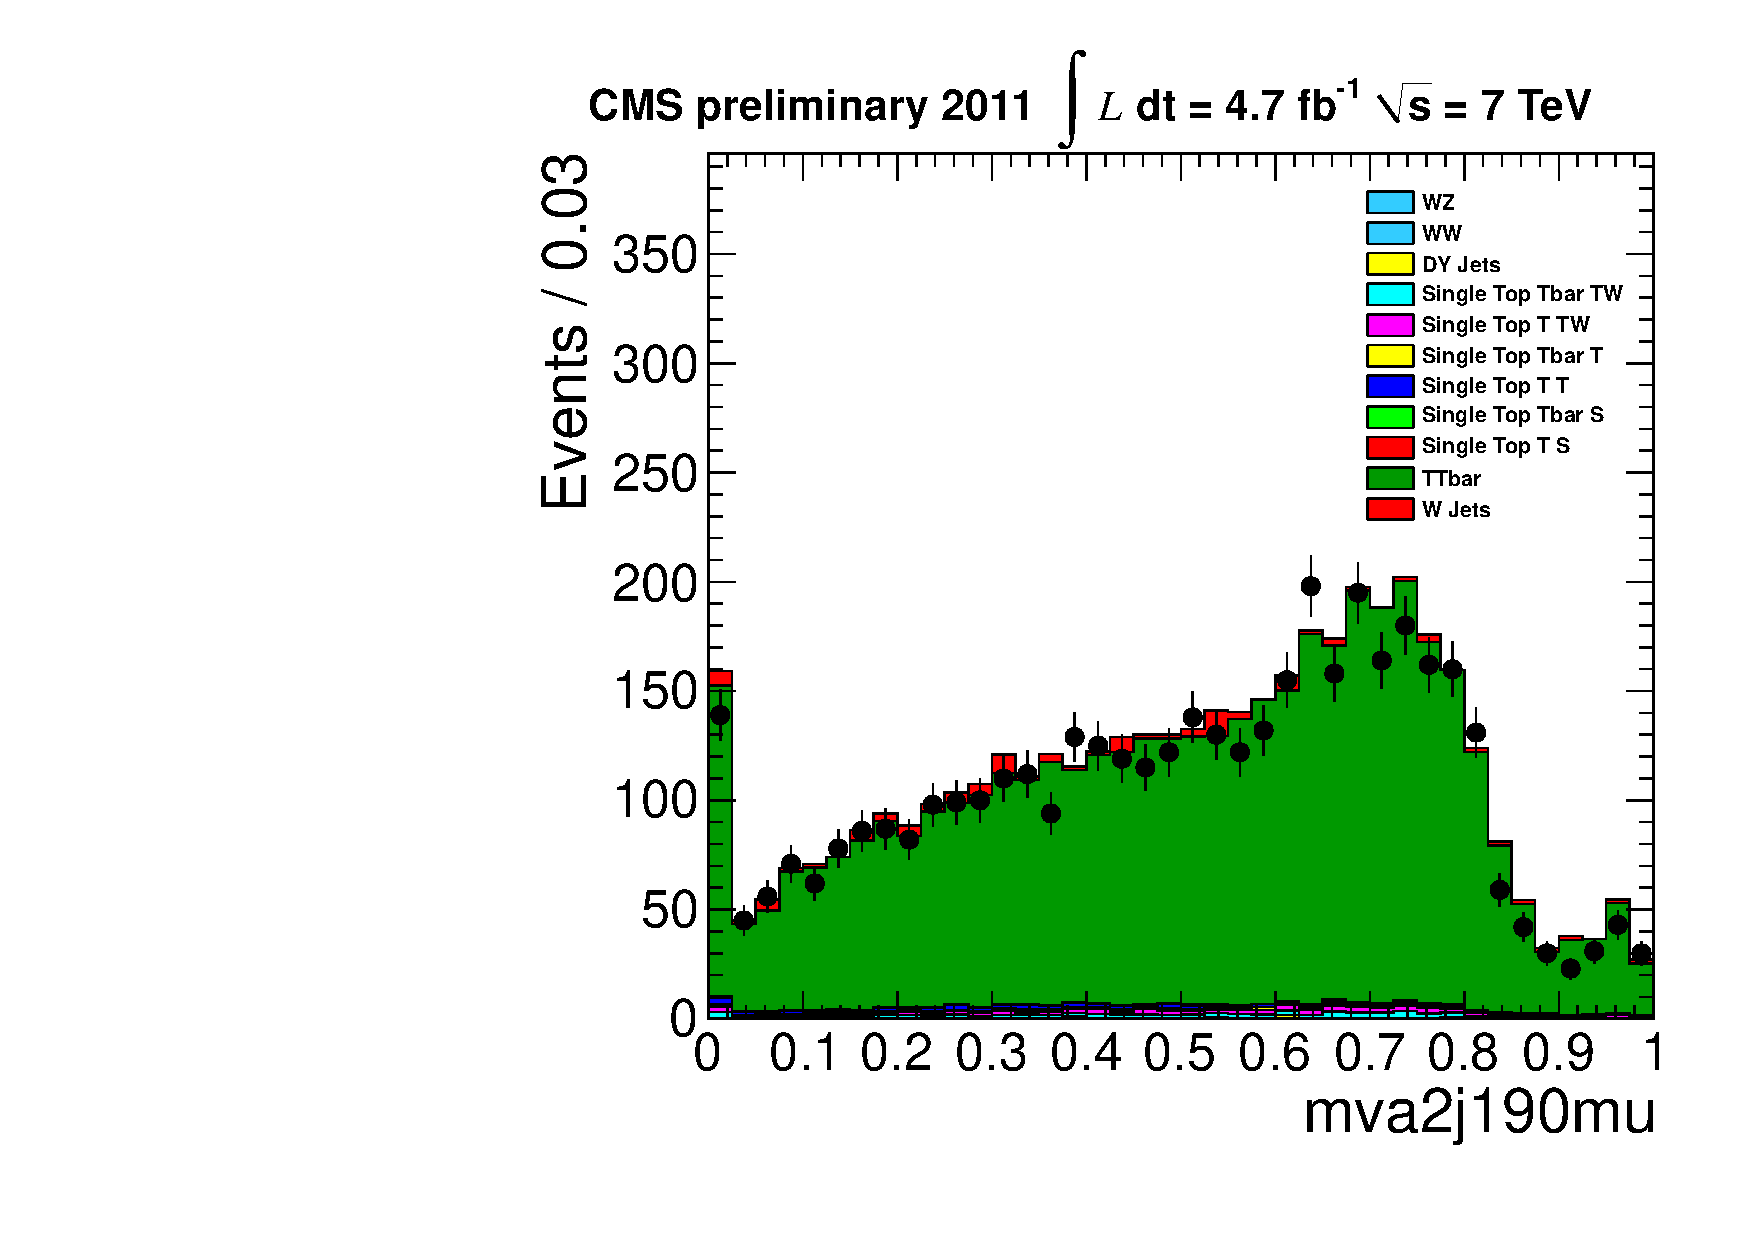
\includegraphics[width=0.49\textwidth]{figs/cl-mva2j190mu-inTTbar.pdf}
  \caption{\label{fig:mva:plots-mva2j190mu} The data-MC comparisons
    after standard event selection (left) and top pair
    selection (right) for the working point: mva2j190mu.}
\end{figure}

%%%%%%%%%%%%%%%%%%% mva2j200mu
\begin{figure}[!t]
  \centering
  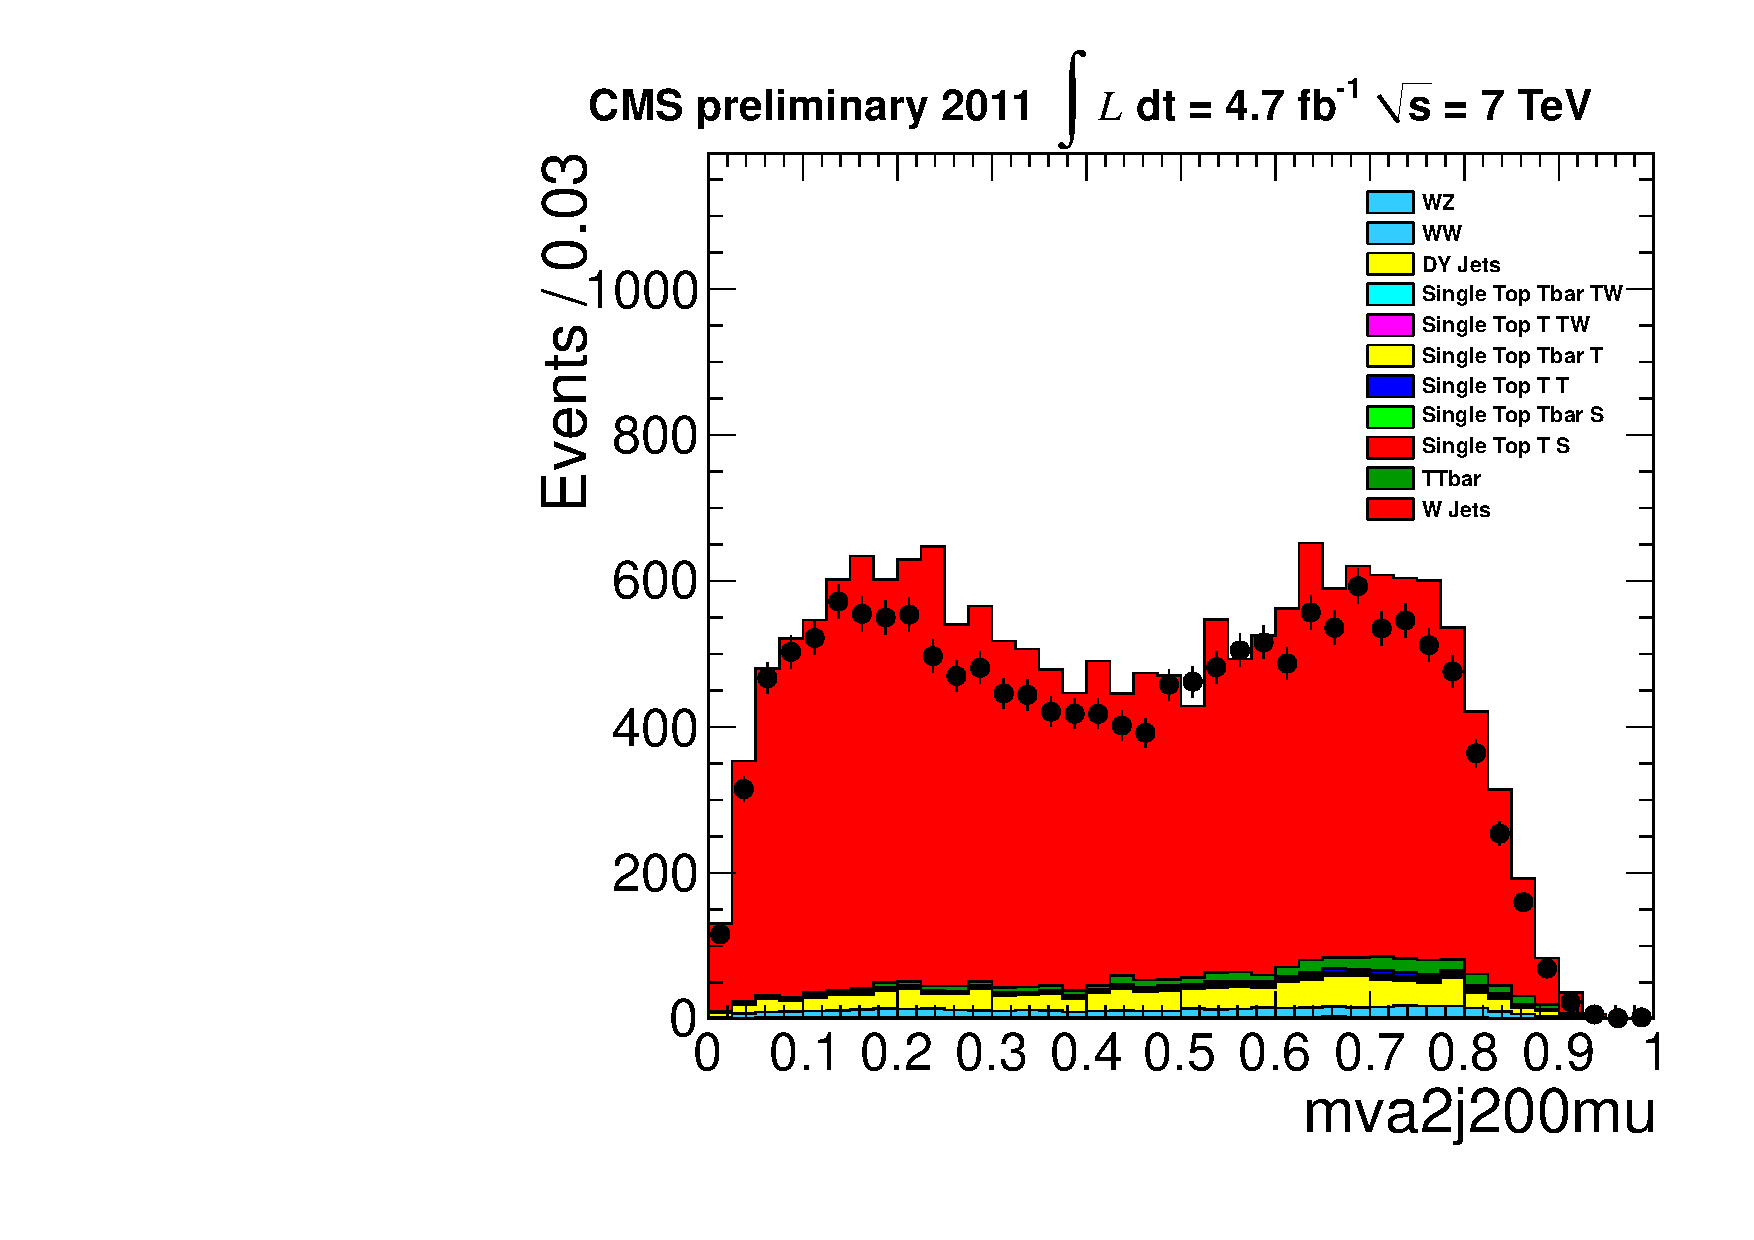
\includegraphics[width=0.49\textwidth]{figs/cl-mva2j200mu-normal.pdf}
  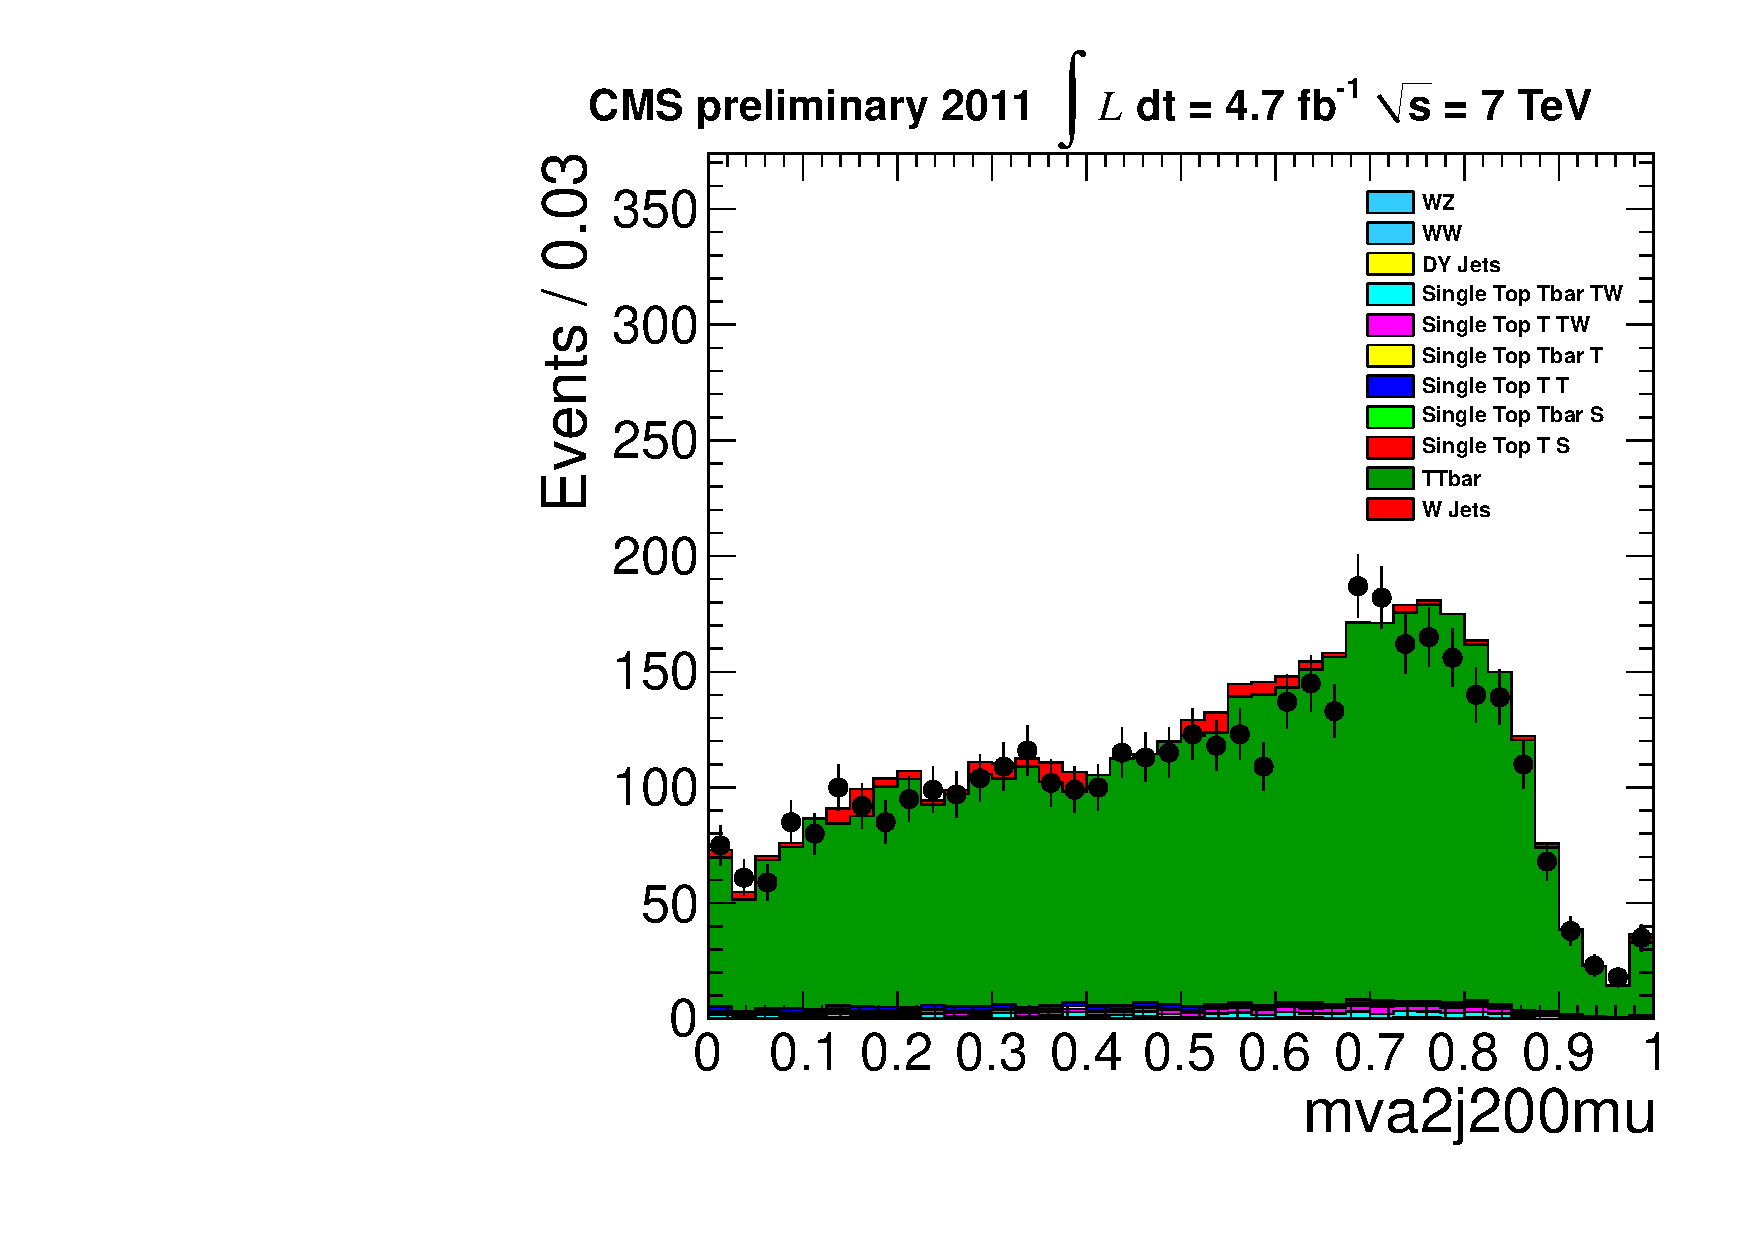
\includegraphics[width=0.49\textwidth]{figs/cl-mva2j200mu-inTTbar.pdf}
  \caption{\label{fig:mva:plots-mva2j200mu} The data-MC comparisons
    after standard event selection (left) and top pair
    selection (right) for the working point: mva2j200mu.}
\end{figure}

%%%%%%%%%%%%%%%%%%% mva2j250mu
\begin{figure}[!t]
  \centering
  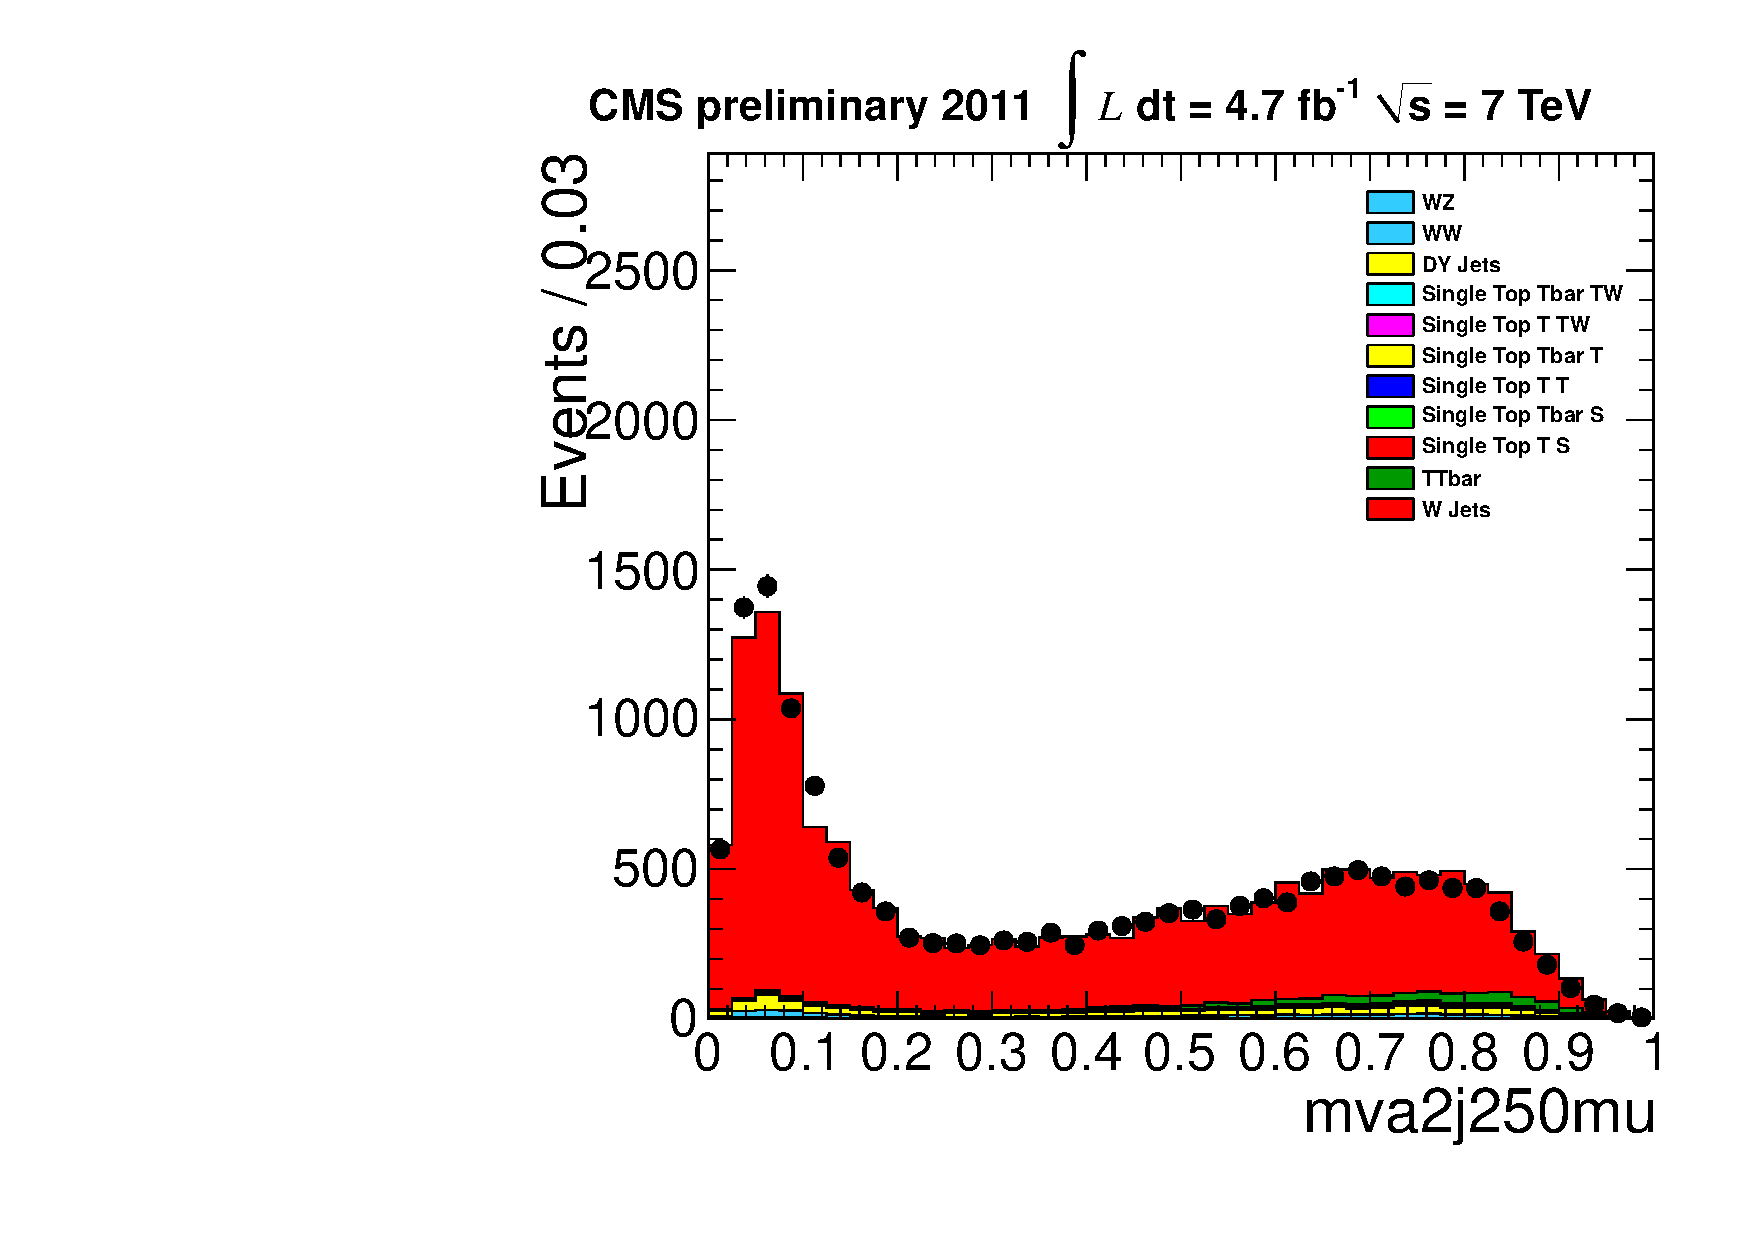
\includegraphics[width=0.49\textwidth]{figs/cl-mva2j250mu-normal.pdf}
  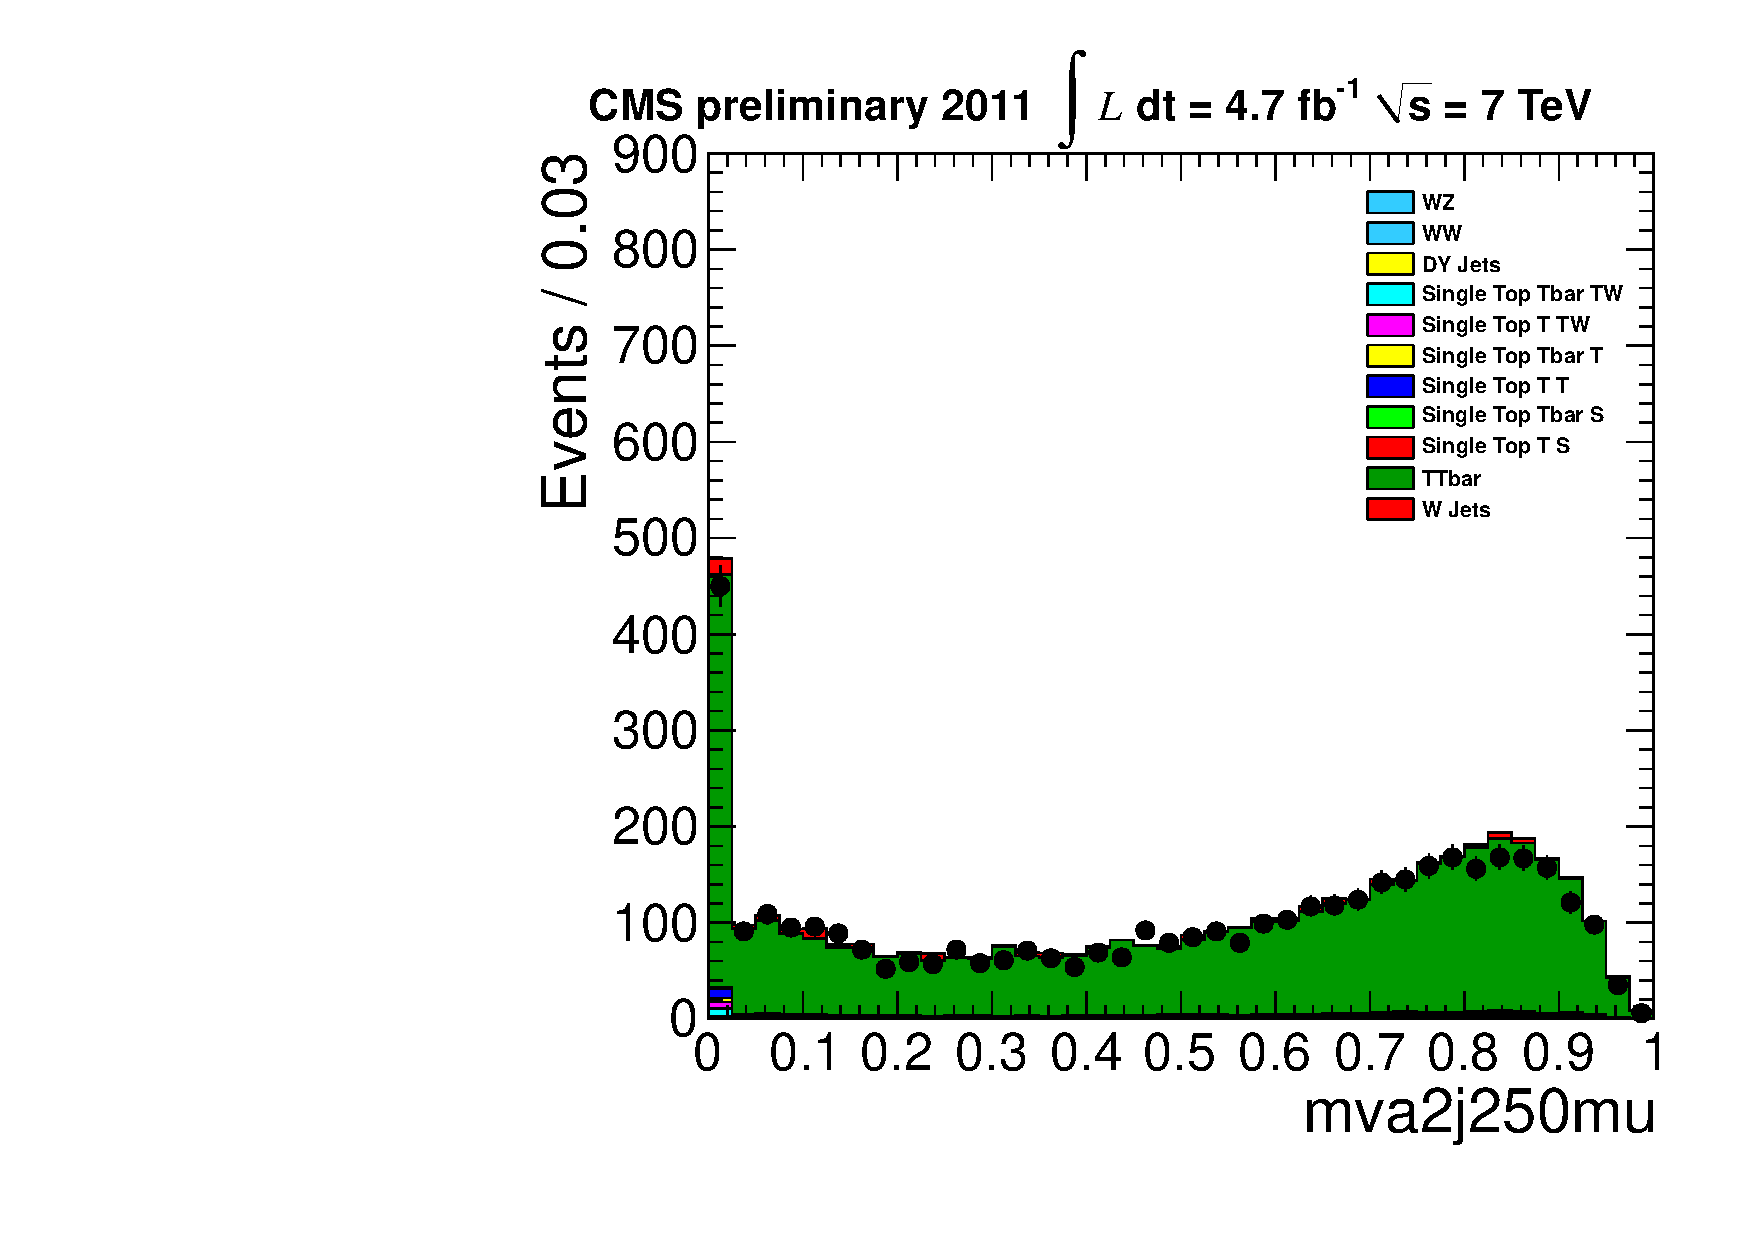
\includegraphics[width=0.49\textwidth]{figs/cl-mva2j250mu-inTTbar.pdf}
  \caption{\label{fig:mva:plots-mva2j250mu} The data-MC comparisons
    after standard event selection (left) and top pair
    selection (right) for the working point: mva2j250mu.}
\end{figure}

%%%%%%%%%%%%%%%%%%% mva2j300mu
\begin{figure}[!t]
  \centering
  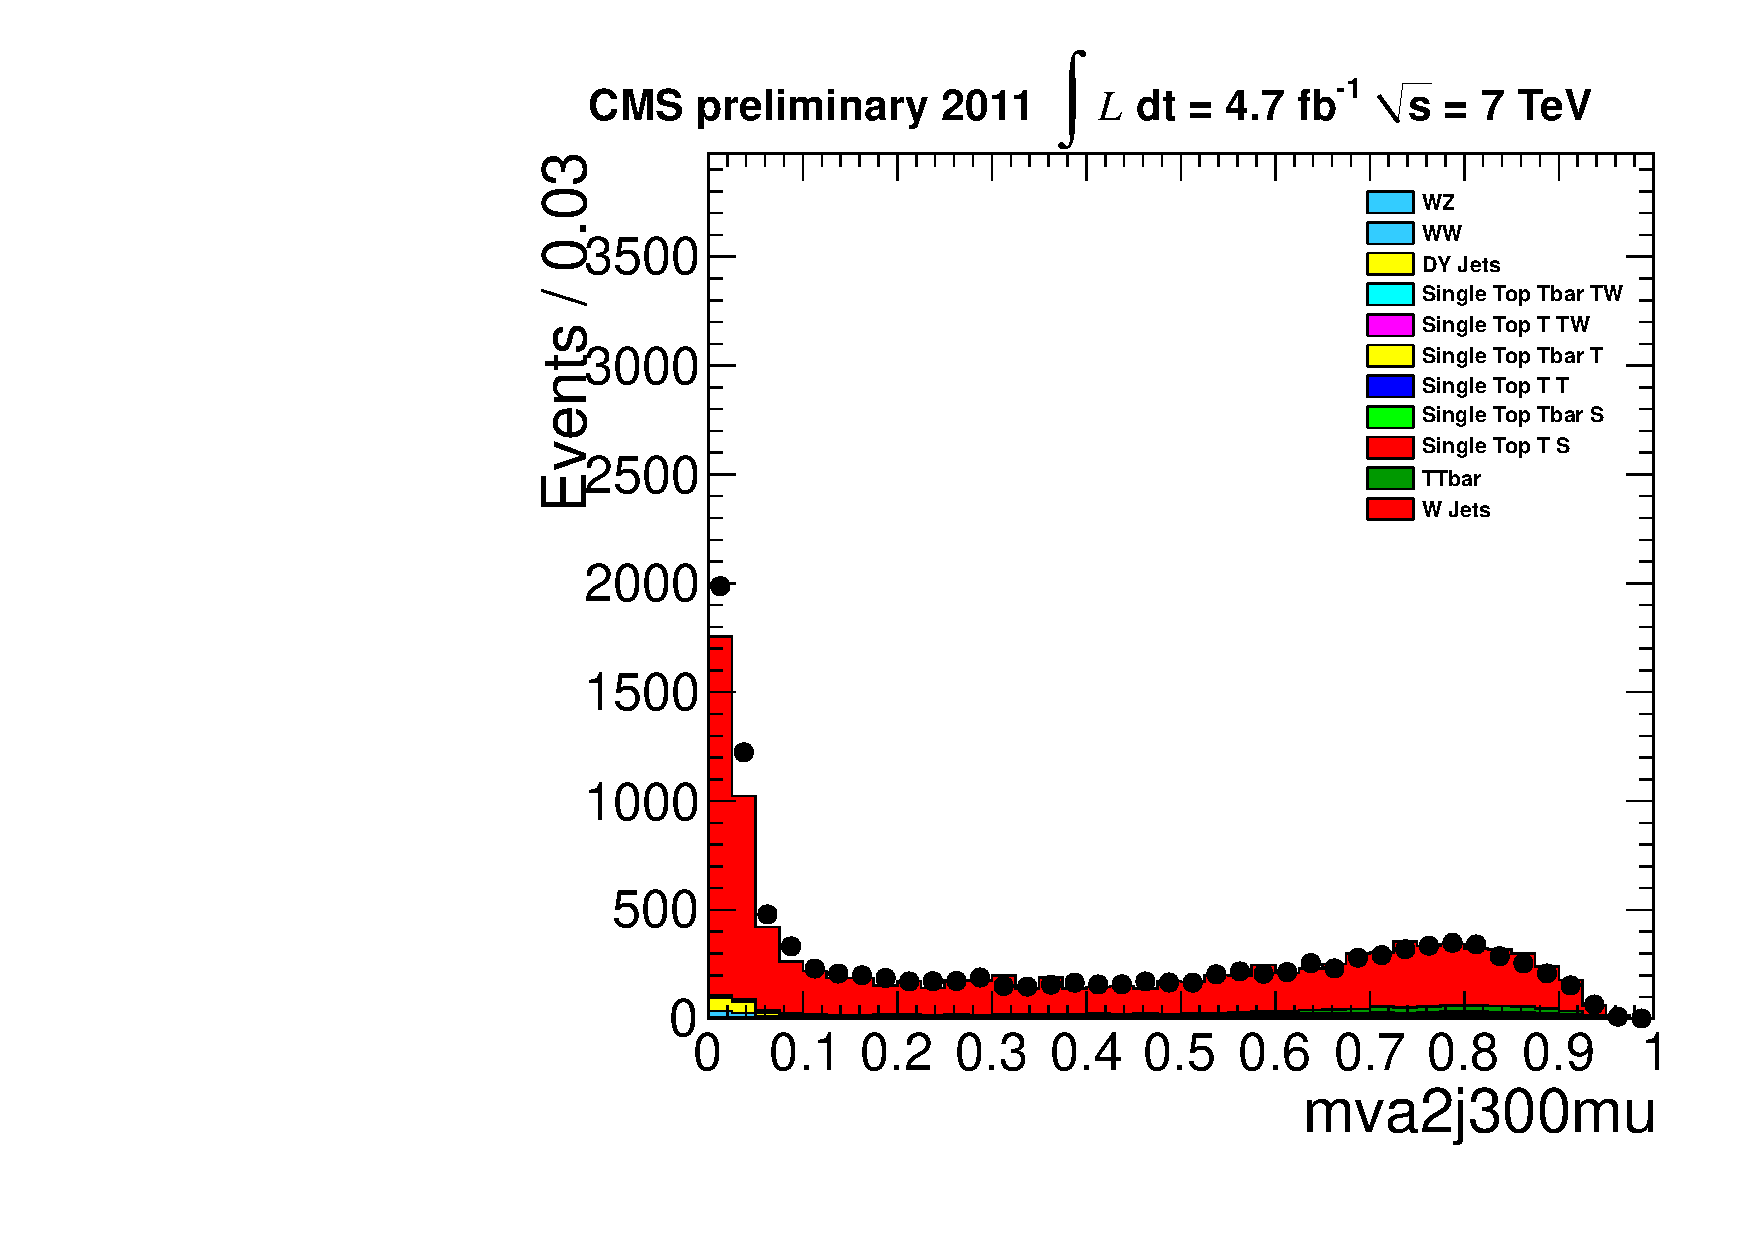
\includegraphics[width=0.49\textwidth]{figs/cl-mva2j300mu-normal.pdf}
  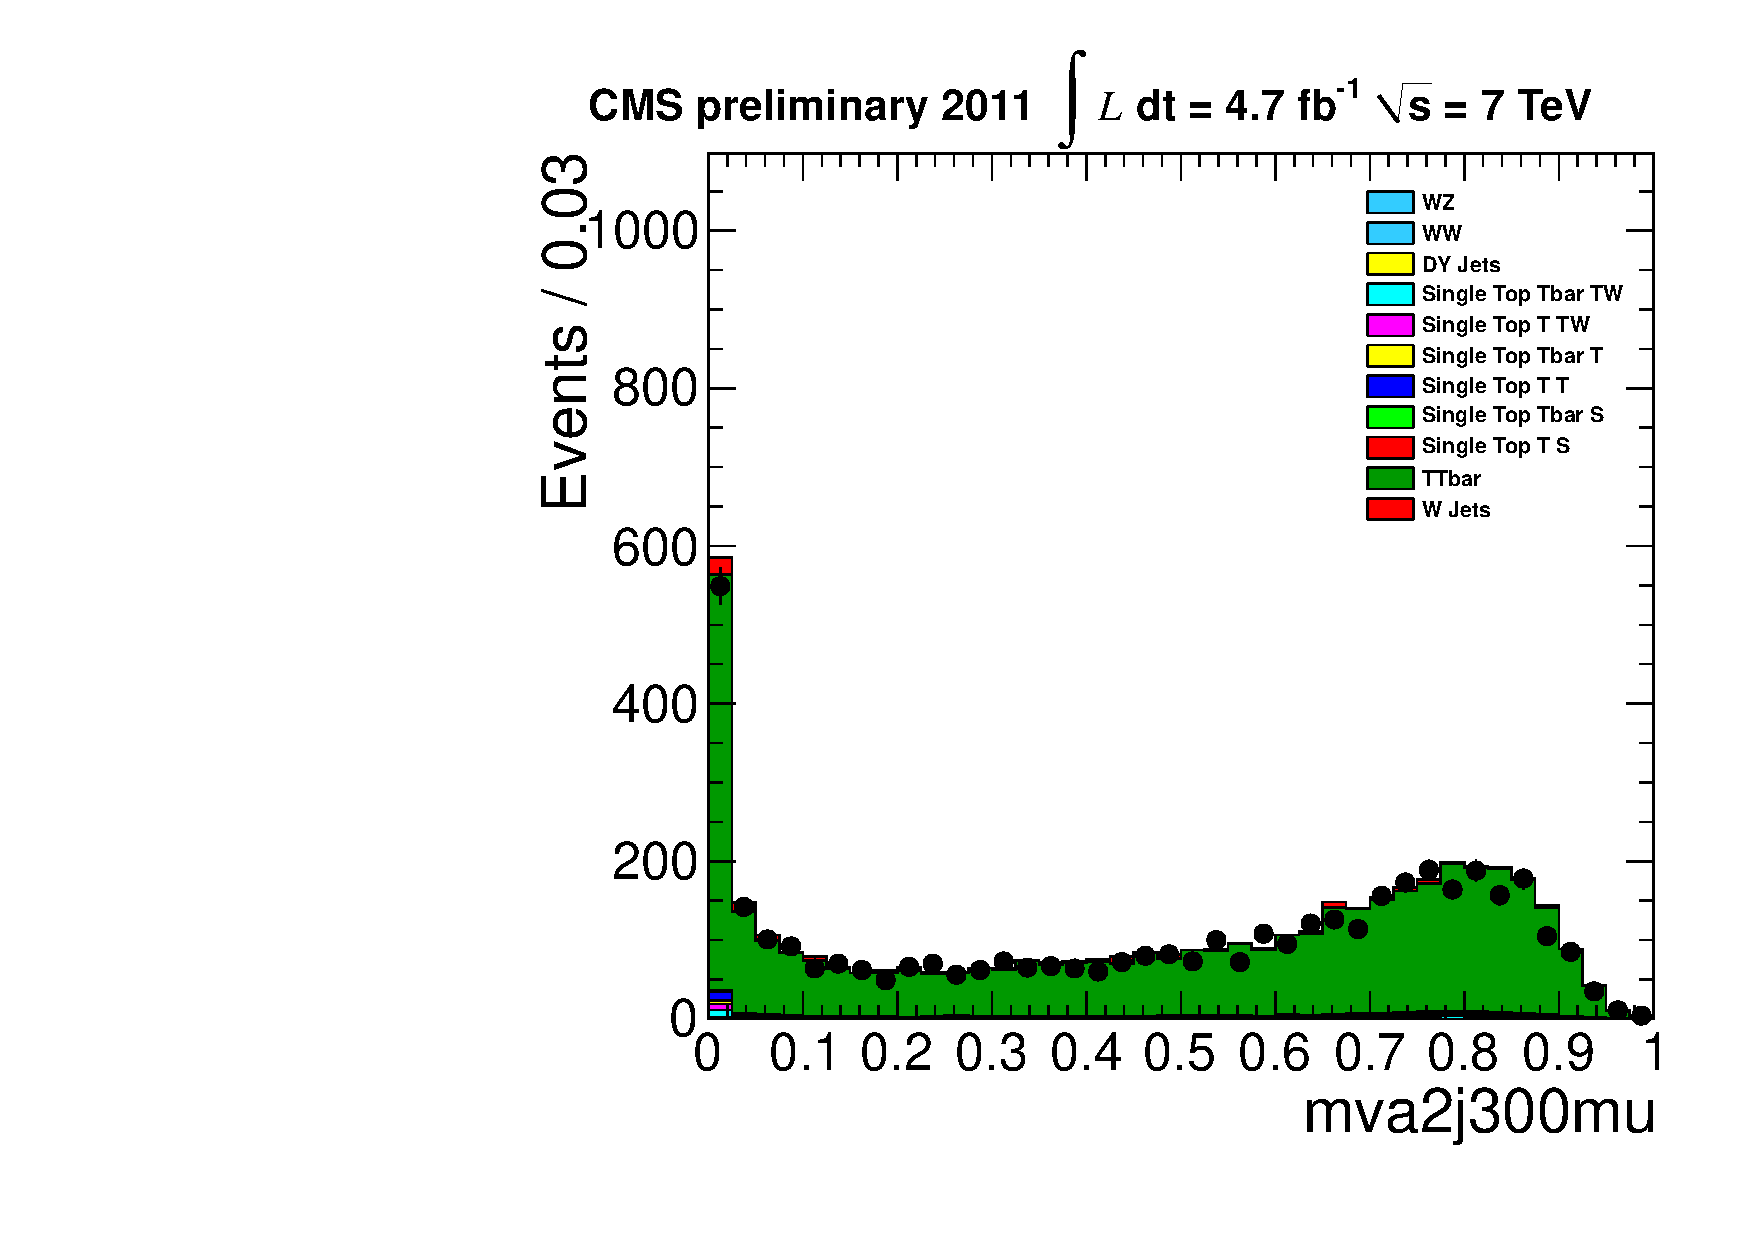
\includegraphics[width=0.49\textwidth]{figs/cl-mva2j300mu-inTTbar.pdf}
  \caption{\label{fig:mva:plots-mva2j300mu} The data-MC comparisons
    after standard event selection (left) and top pair
    selection (right) for the working point: mva2j300mu.}
\end{figure}

%%%%%%%%%%%%%%%%%%% mva2j350mu
\begin{figure}[!t]
  \centering
  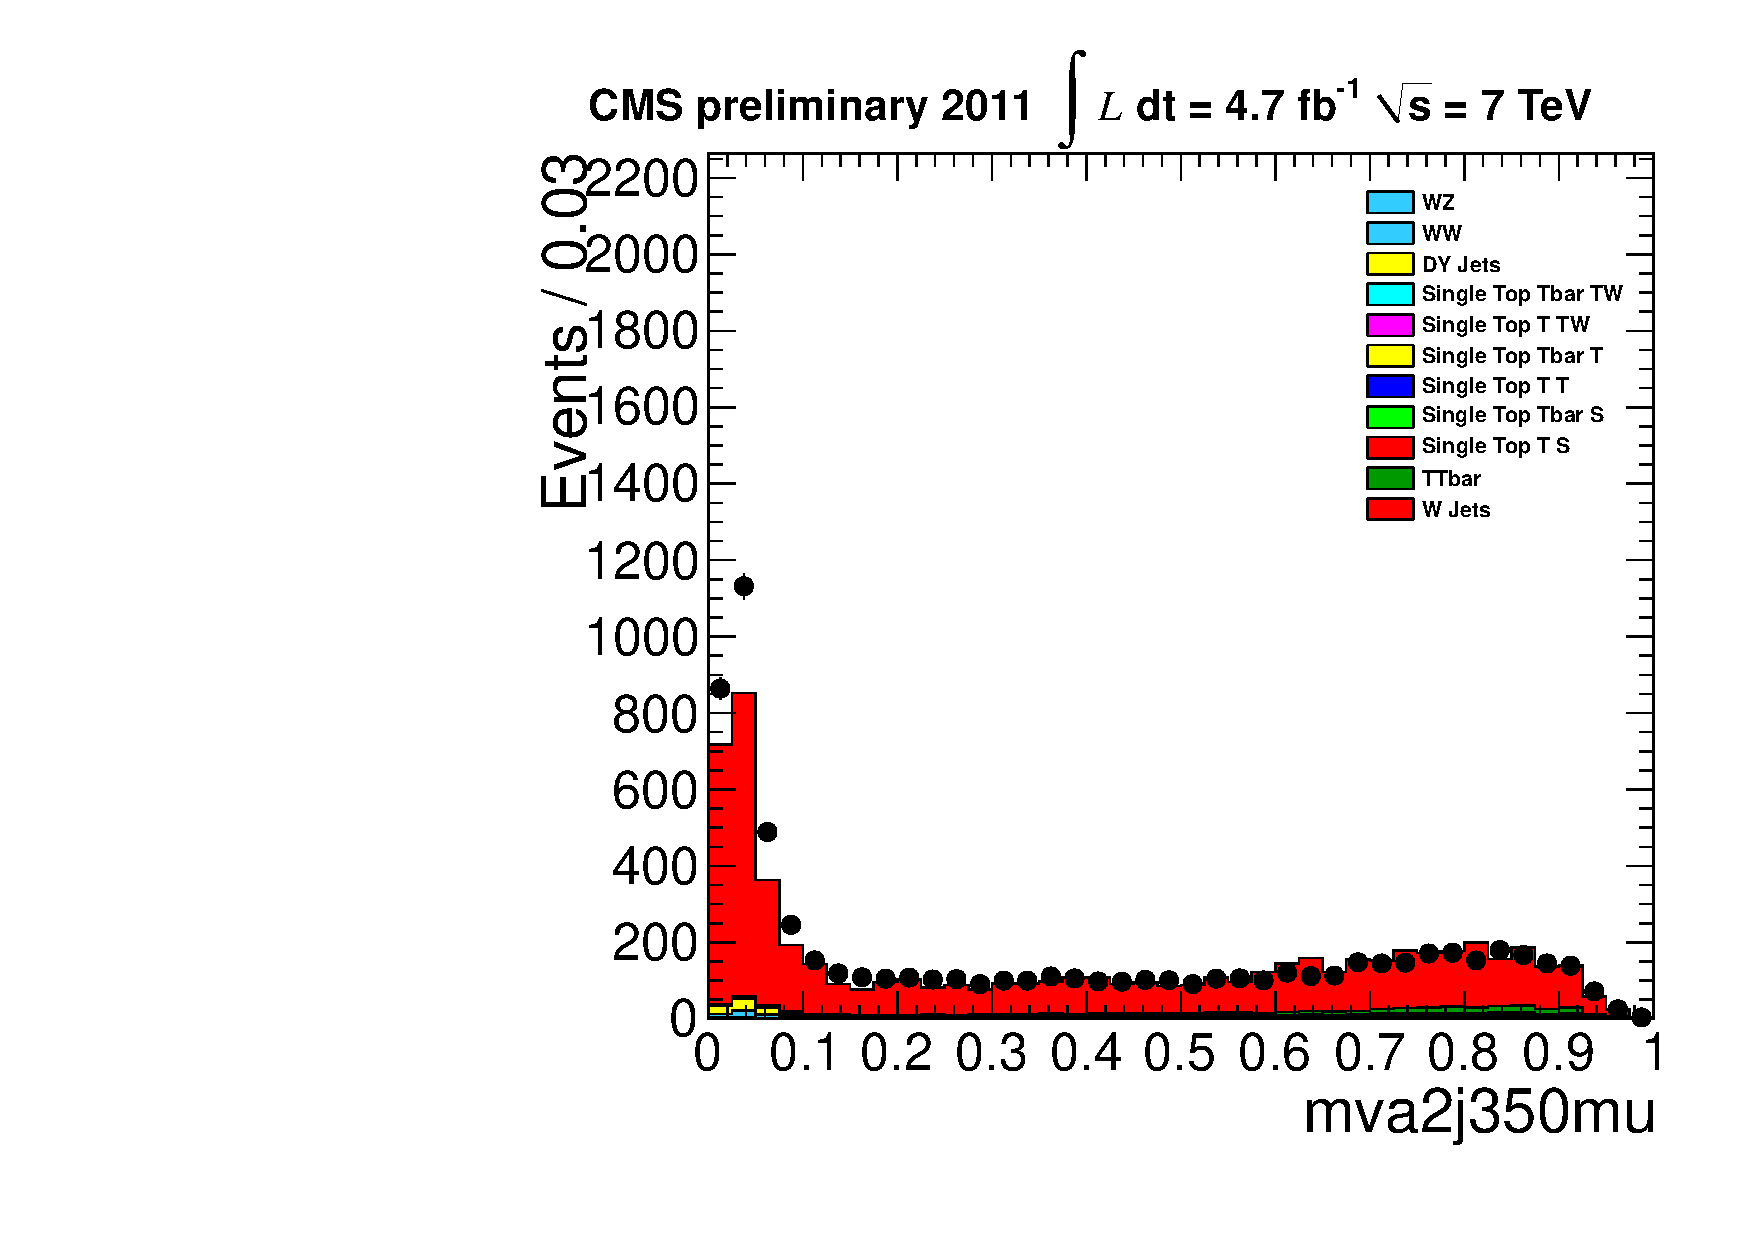
\includegraphics[width=0.49\textwidth]{figs/cl-mva2j350mu-normal.pdf}
  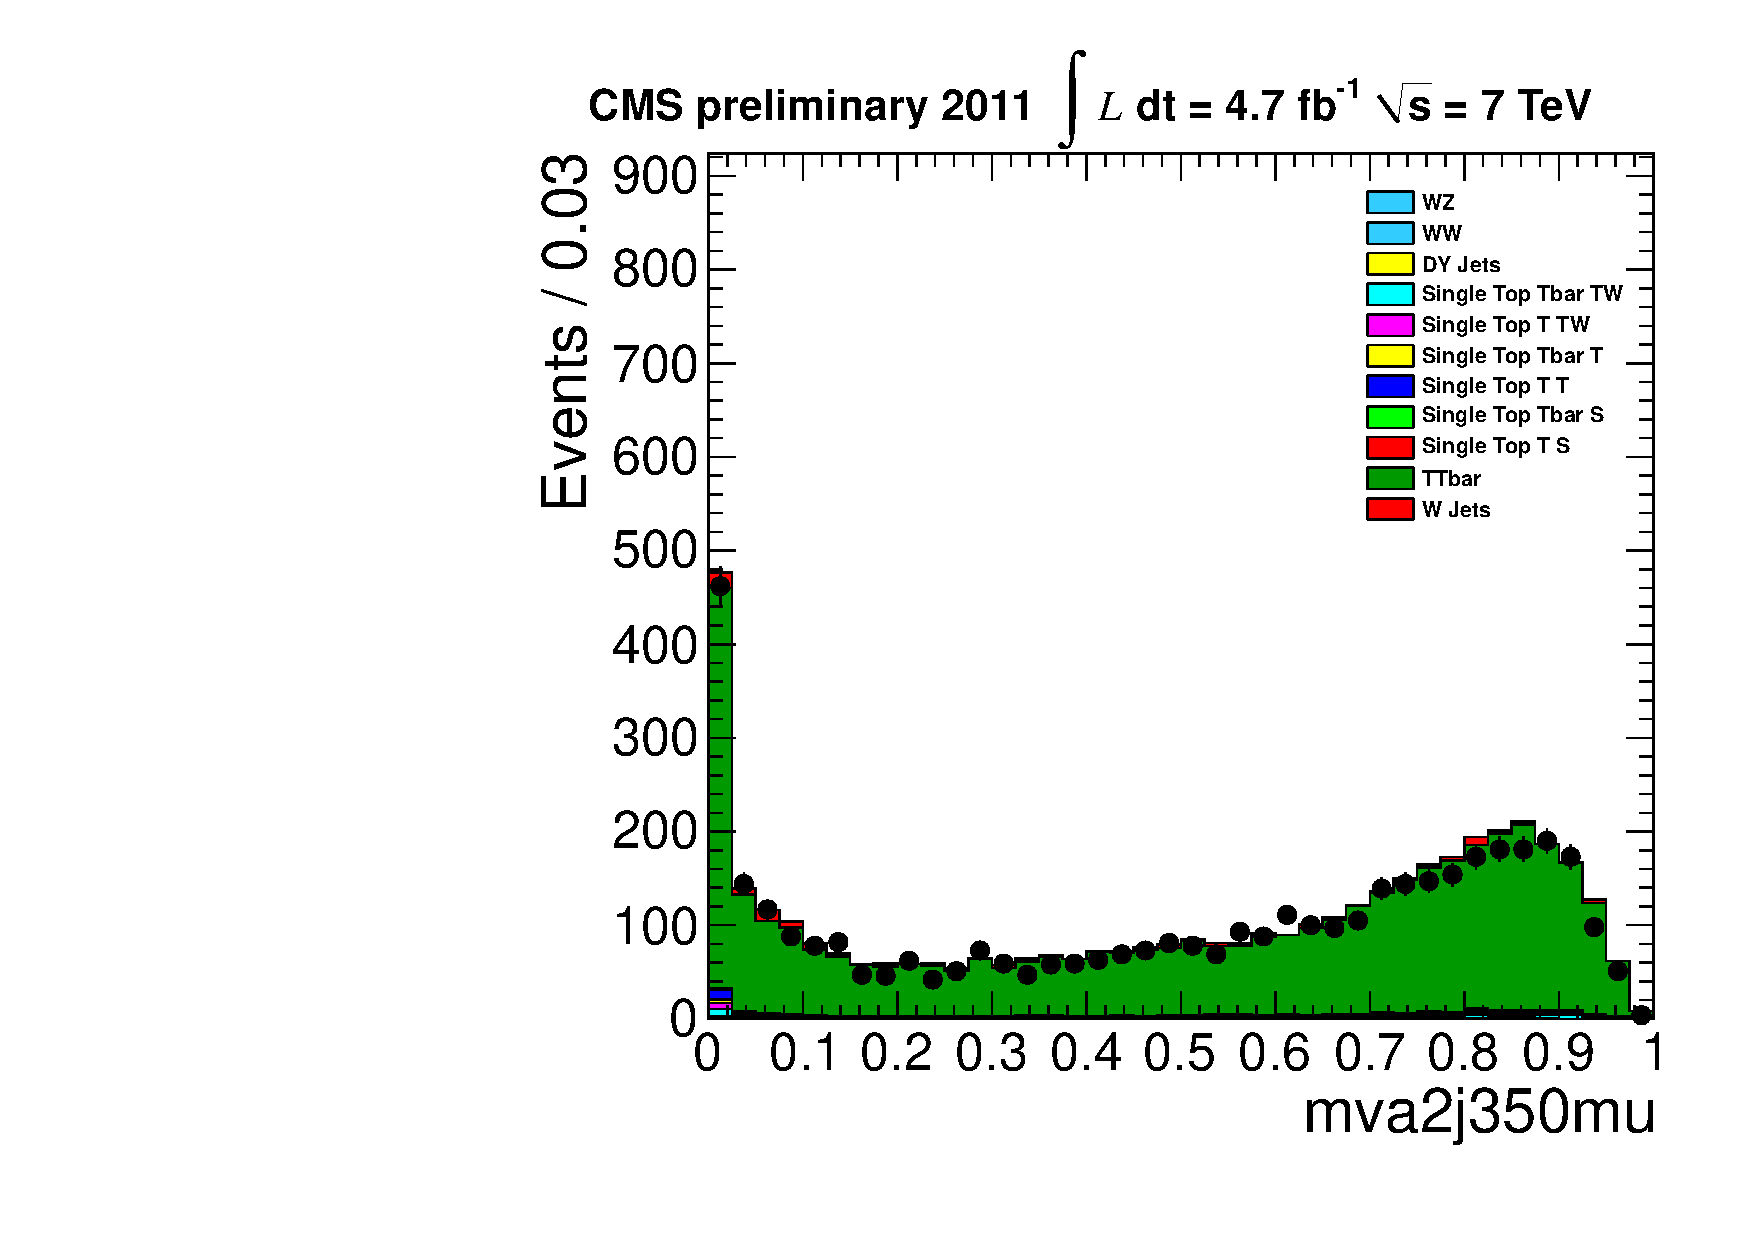
\includegraphics[width=0.49\textwidth]{figs/cl-mva2j350mu-inTTbar.pdf}
  \caption{\label{fig:mva:plots-mva2j350mu} The data-MC comparisons
    after standard event selection (left) and top pair
    selection (right) for the working point: mva2j350mu.}
\end{figure}

%%%%%%%%%%%%%%%%%%% mva2j400mu
\begin{figure}[!t]
  \centering
  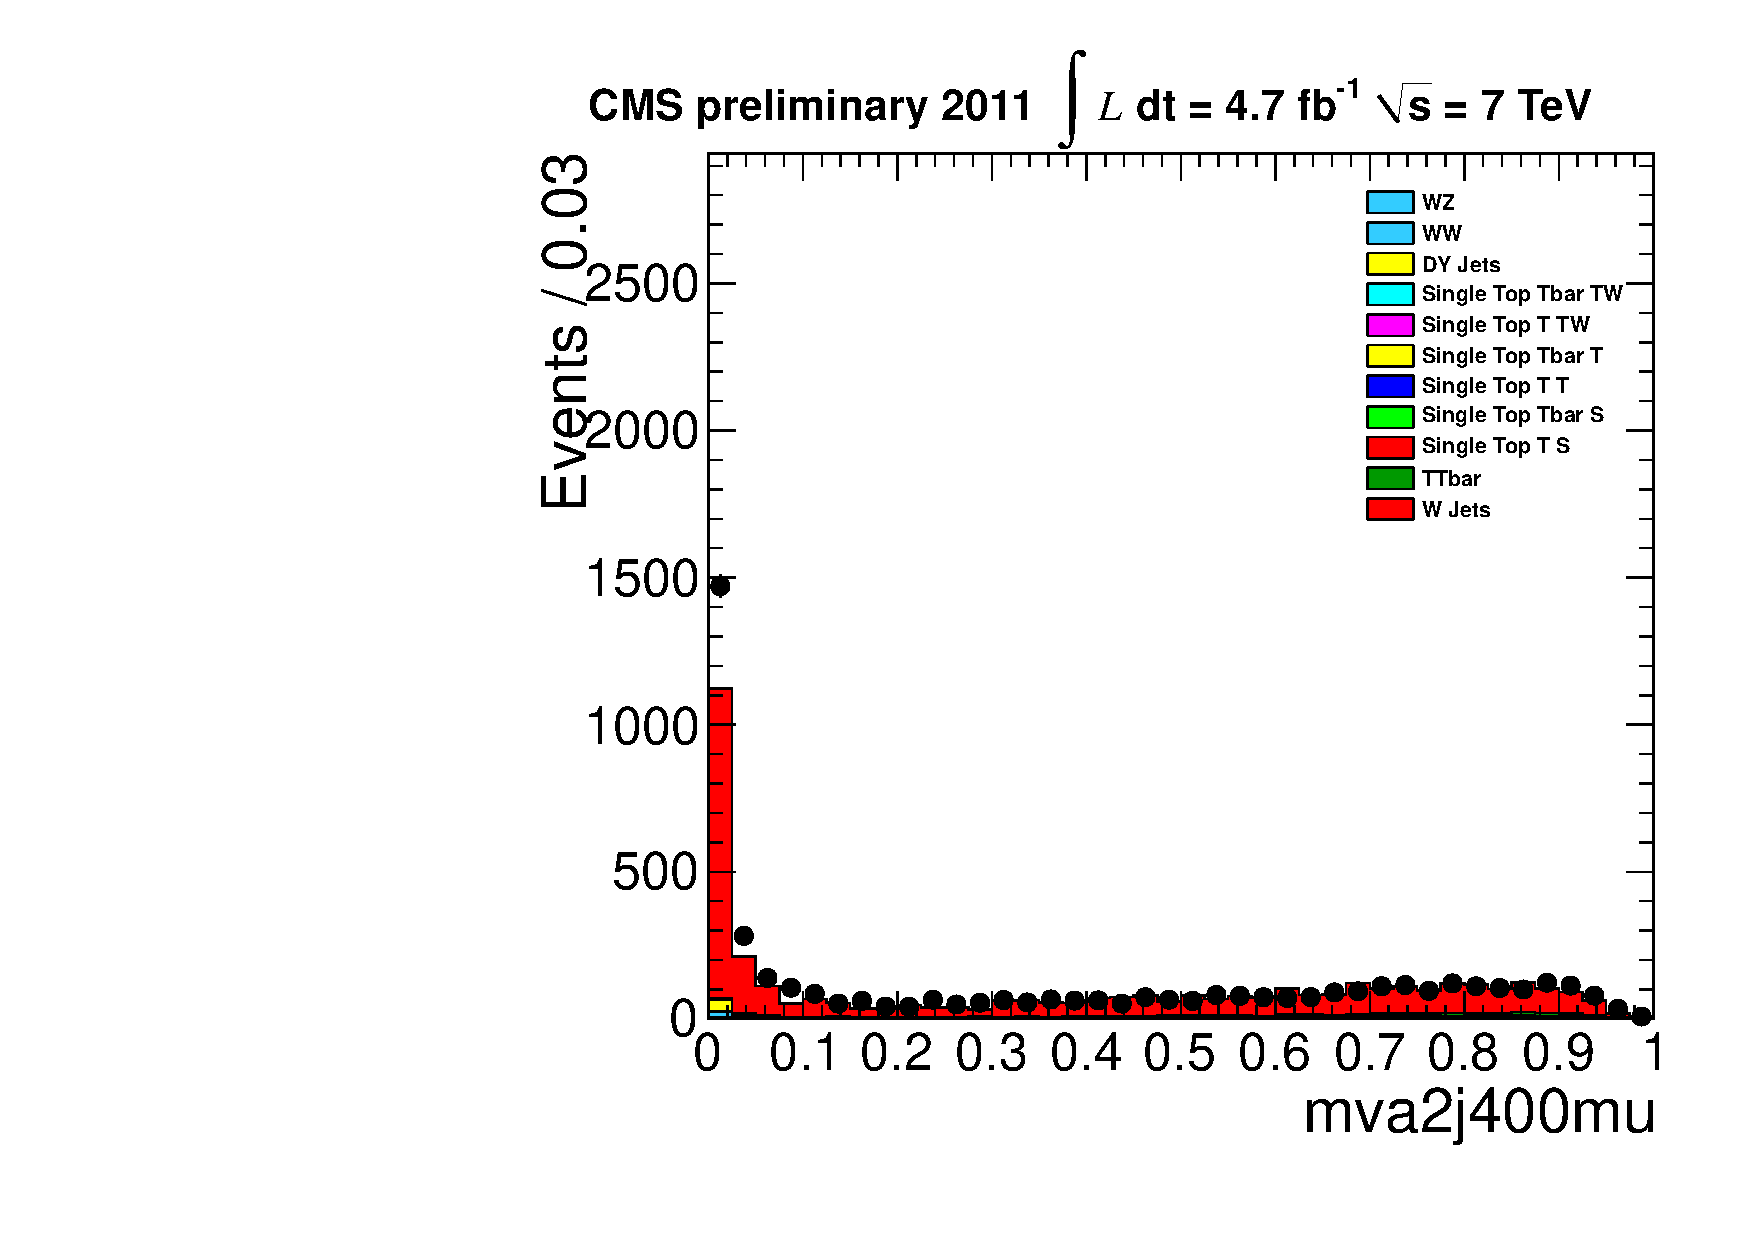
\includegraphics[width=0.49\textwidth]{figs/cl-mva2j400mu-normal.pdf}
  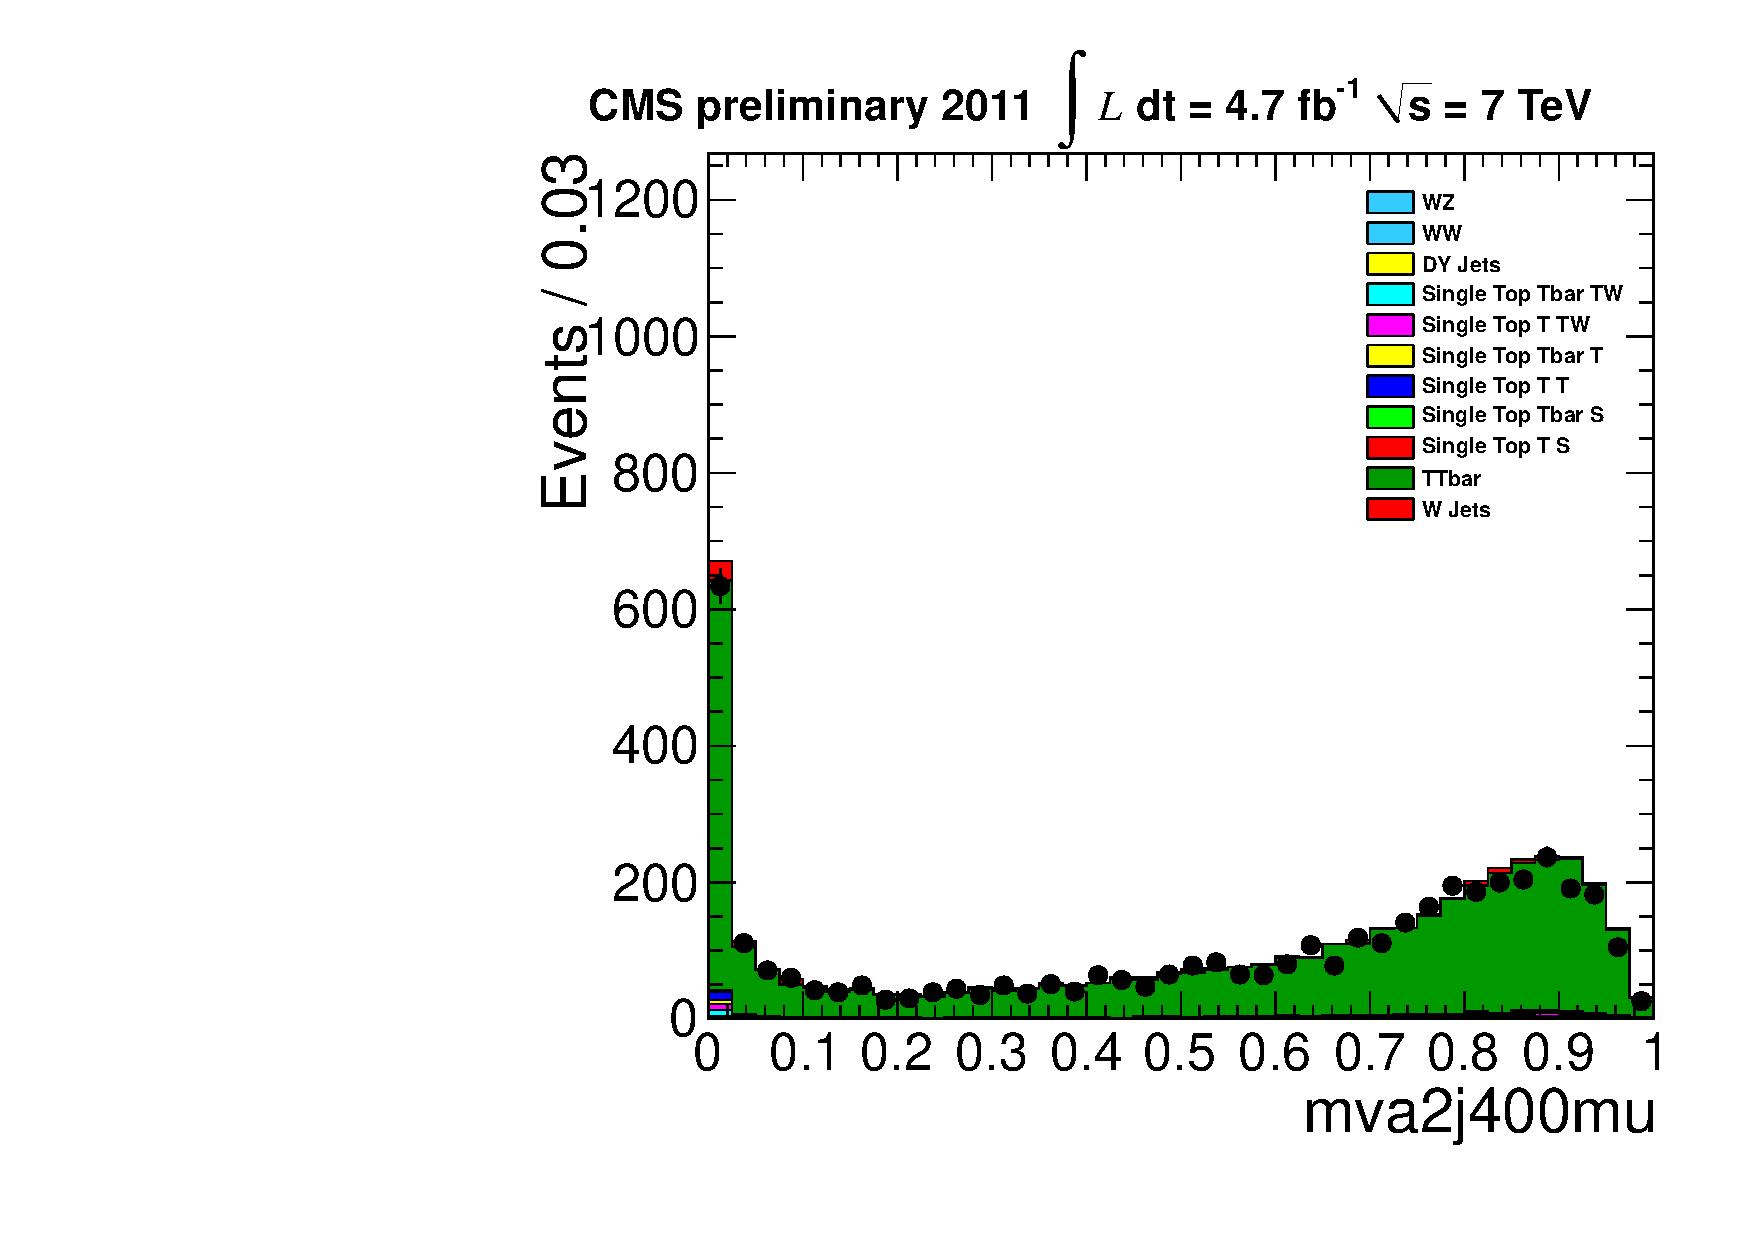
\includegraphics[width=0.49\textwidth]{figs/cl-mva2j400mu-inTTbar.pdf}
  \caption{\label{fig:mva:plots-mva2j400mu} The data-MC comparisons
    after standard event selection (left) and top pair
    selection (right) for the working point: mva2j400mu.}
\end{figure}

%%%%%%%%%%%%%%%%%%% mva2j450mu
\begin{figure}[!t]
  \centering
  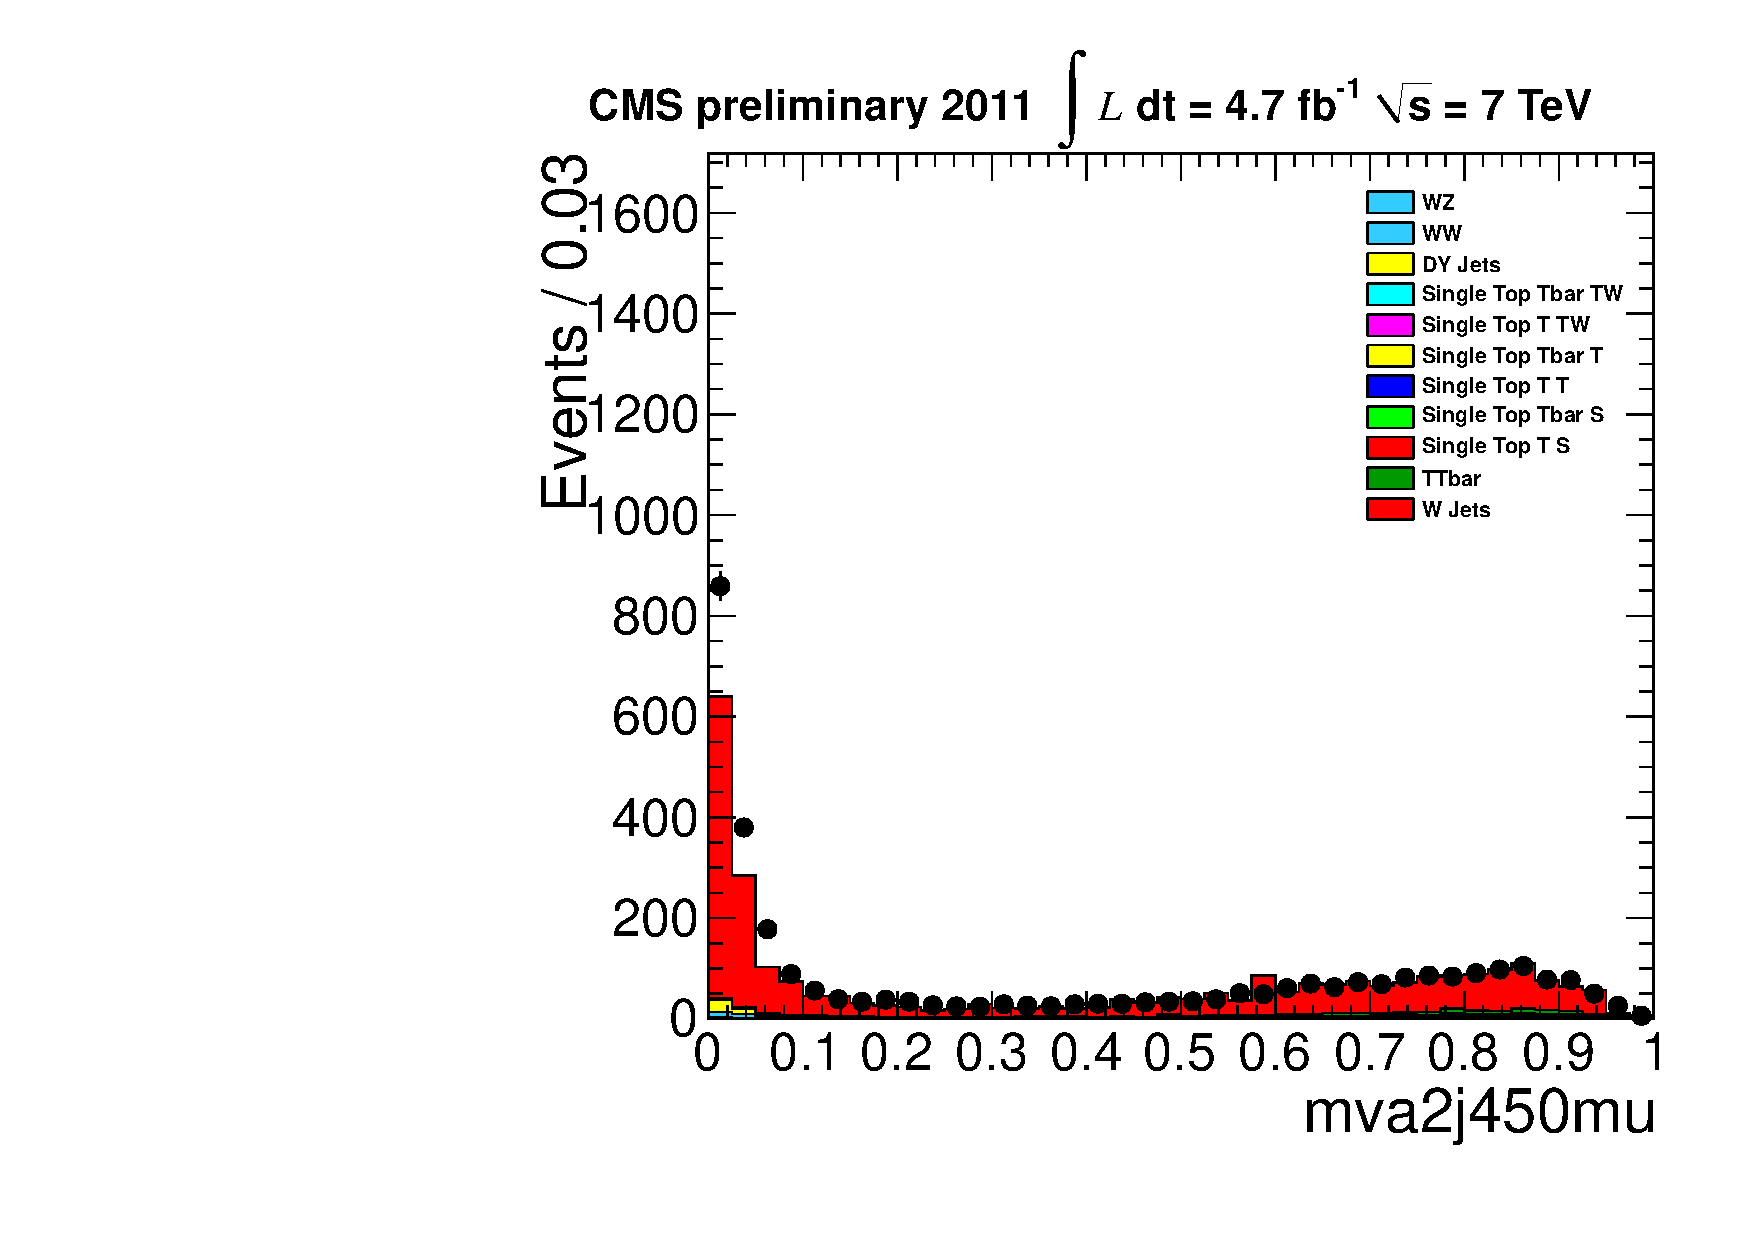
\includegraphics[width=0.49\textwidth]{figs/cl-mva2j450mu-normal.pdf}
  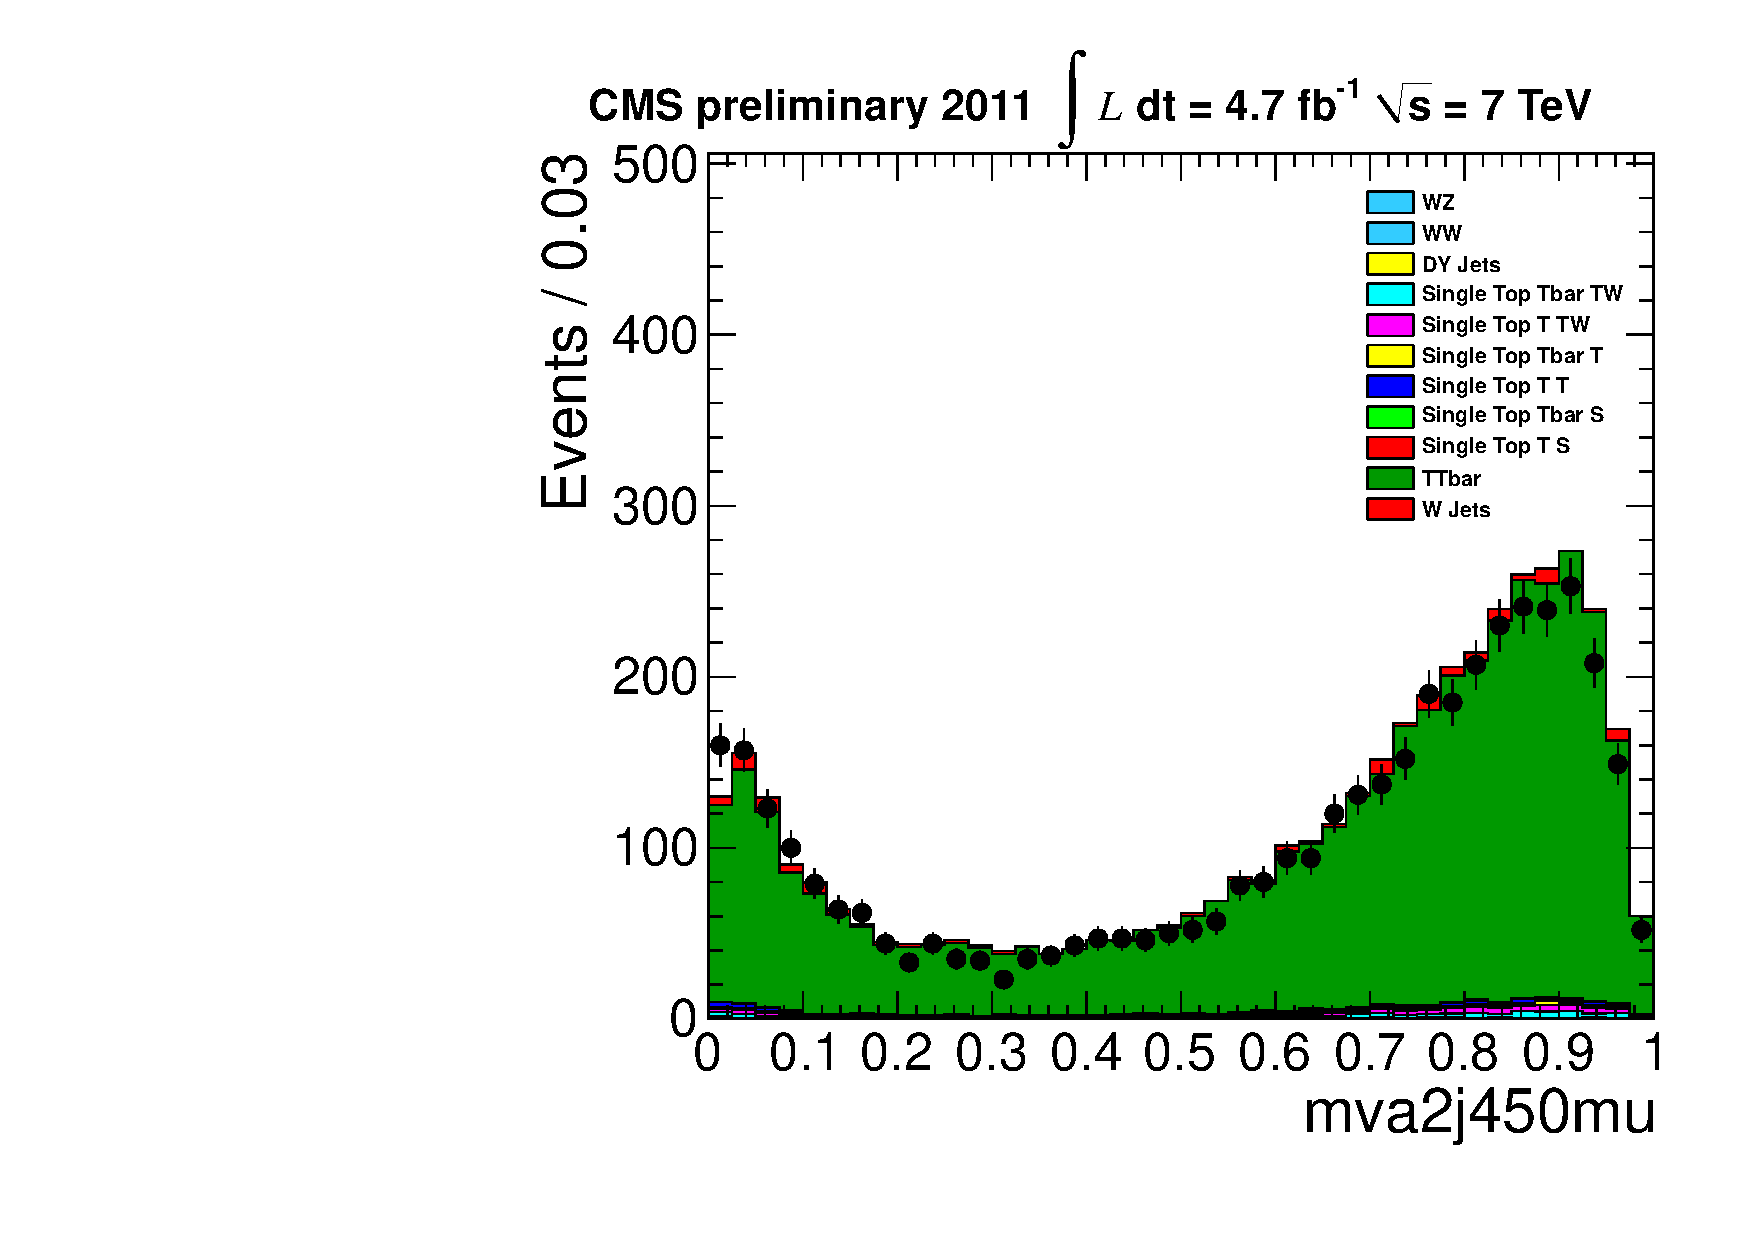
\includegraphics[width=0.49\textwidth]{figs/cl-mva2j450mu-inTTbar.pdf}
  \caption{\label{fig:mva:plots-mva2j450mu} The data-MC comparisons
    after standard event selection (left) and top pair
    selection (right) for the working point: mva2j450mu.}
\end{figure}

%%%%%%%%%%%%%%%%%%% mva2j500mu
\begin{figure}[!t]
  \centering
  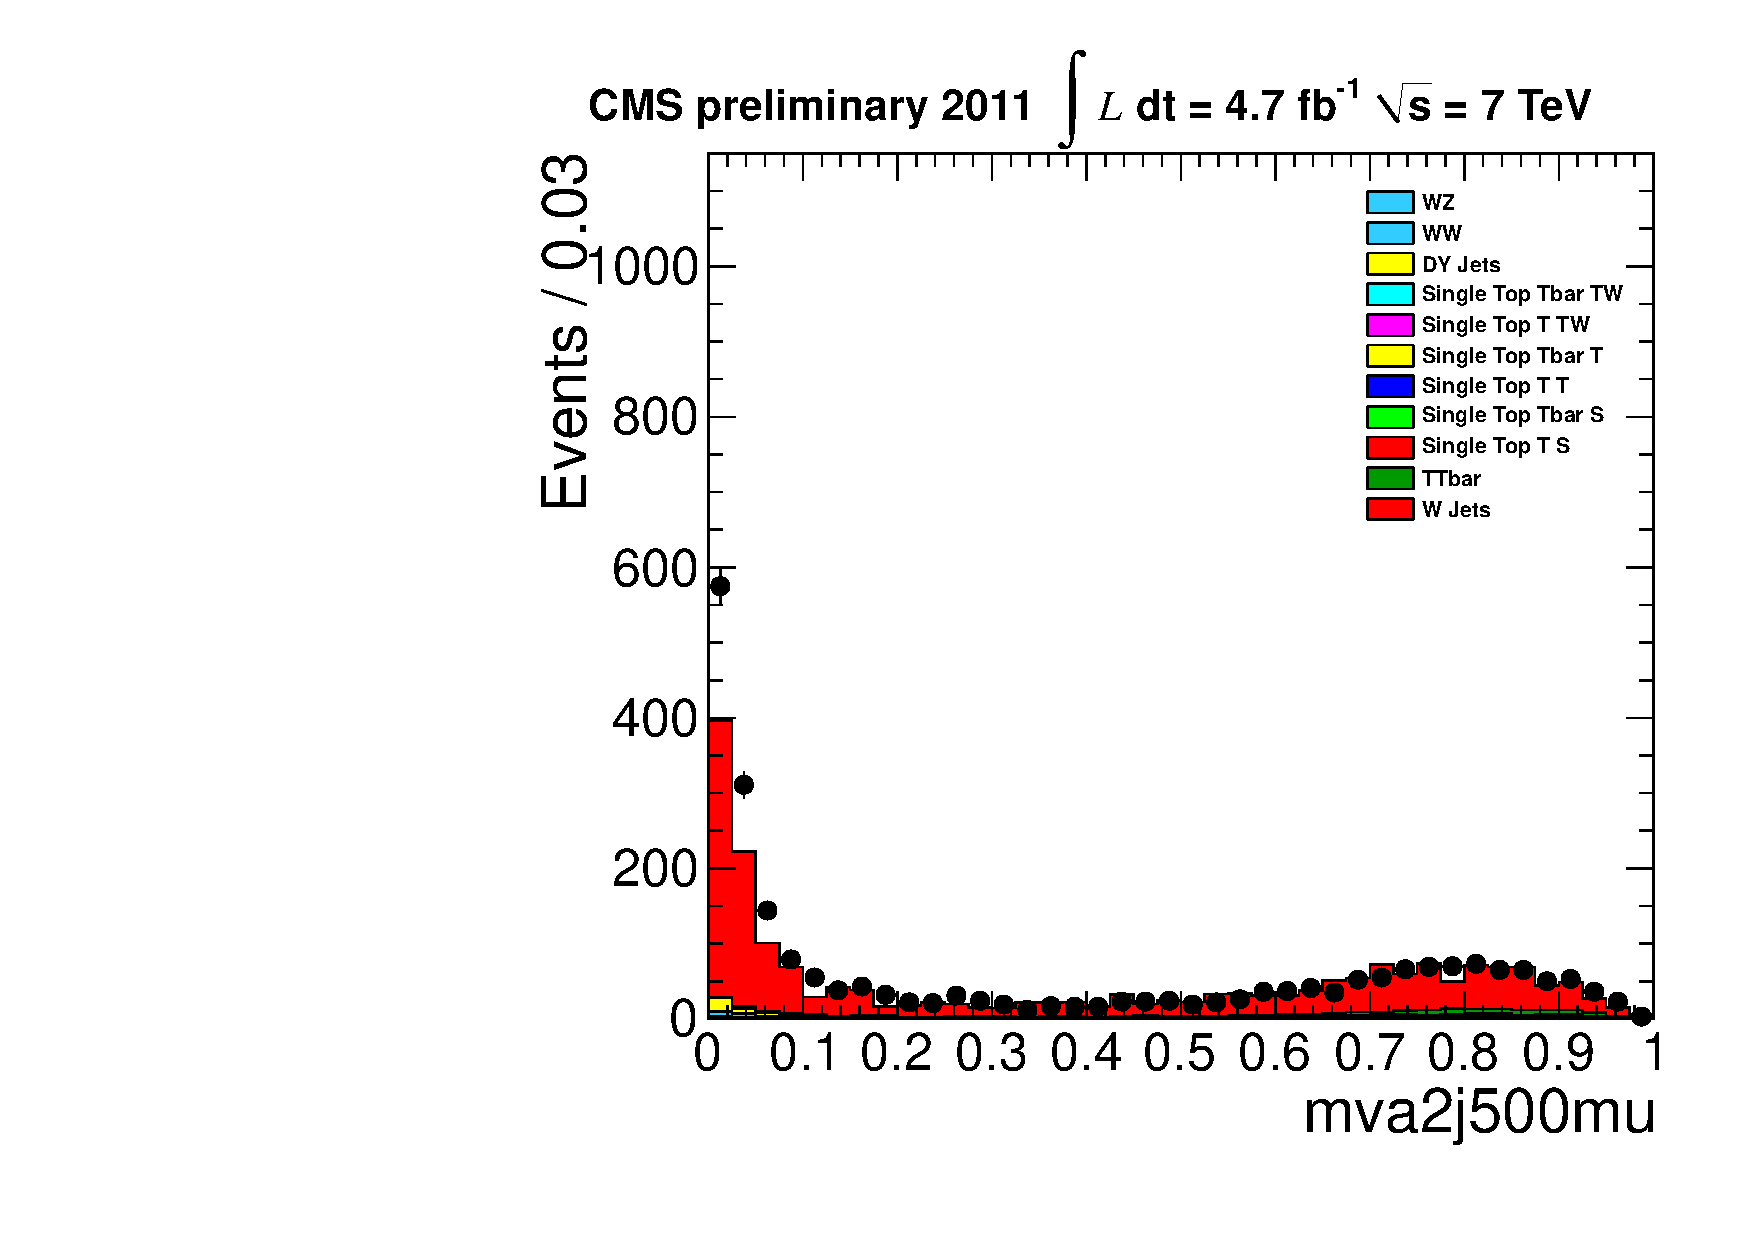
\includegraphics[width=0.49\textwidth]{figs/cl-mva2j500mu-normal.pdf}
  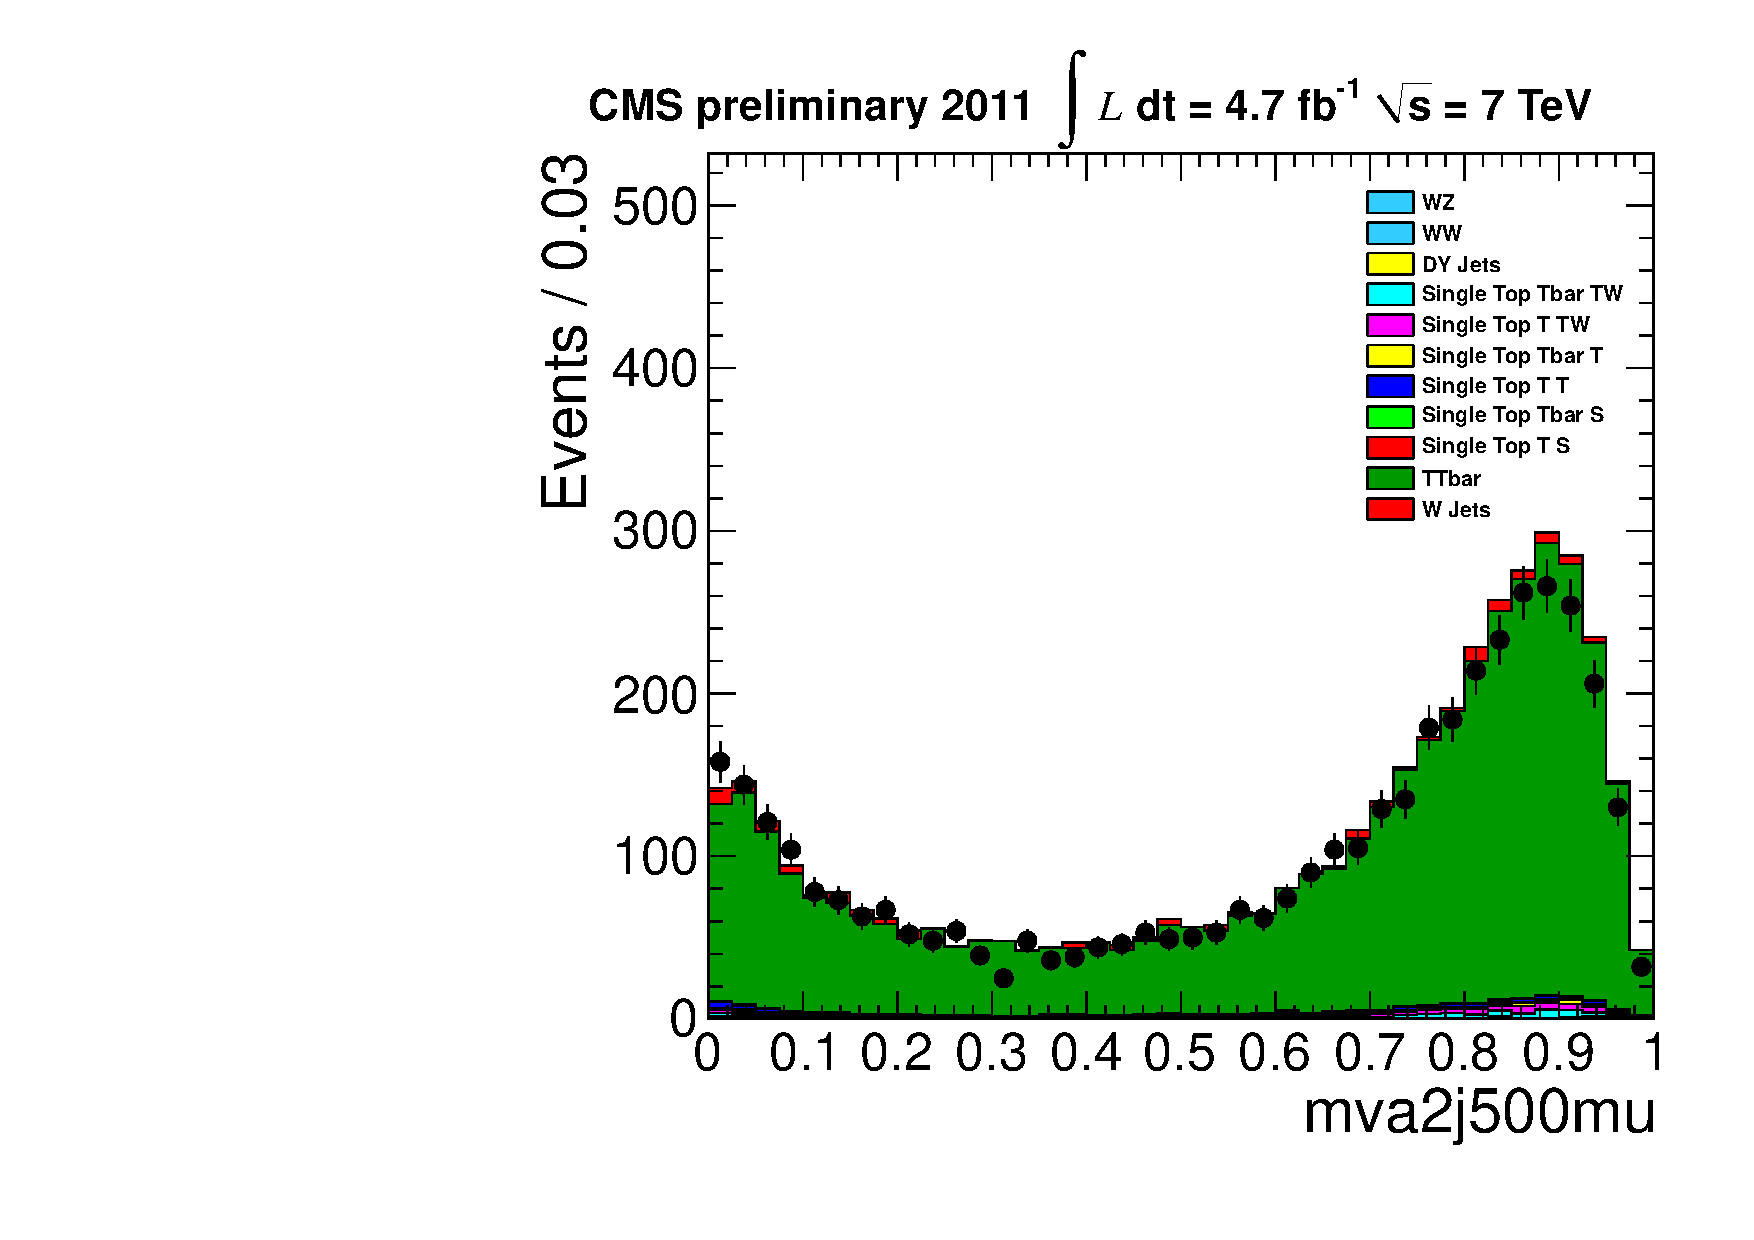
\includegraphics[width=0.49\textwidth]{figs/cl-mva2j500mu-inTTbar.pdf}
  \caption{\label{fig:mva:plots-mva2j500mu} The data-MC comparisons
    after standard event selection (left) and top pair
    selection (right) for the working point: mva2j500mu.}
\end{figure}

%%%%%%%%%%%%%%%%%%% mva2j550mu
\begin{figure}[!t]
  \centering
  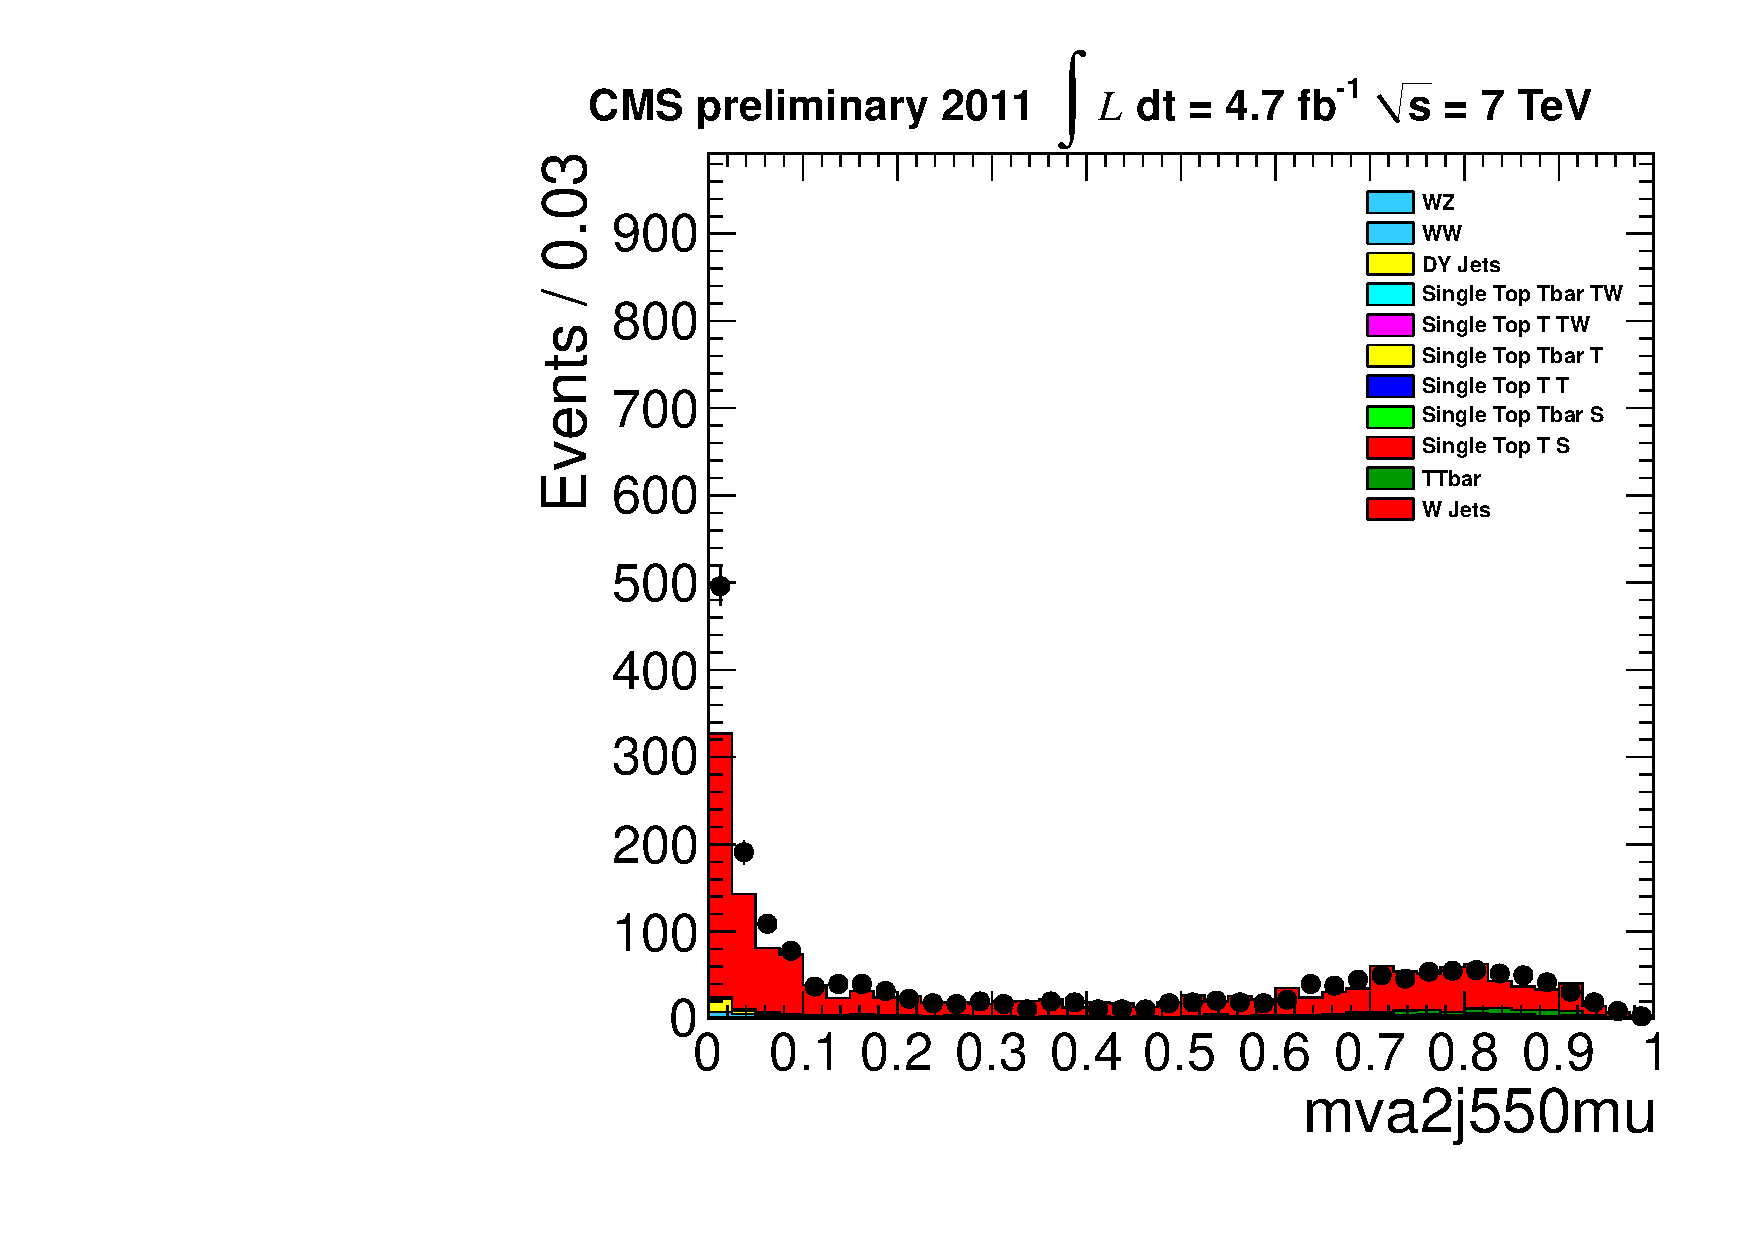
\includegraphics[width=0.49\textwidth]{figs/cl-mva2j550mu-normal.pdf}
  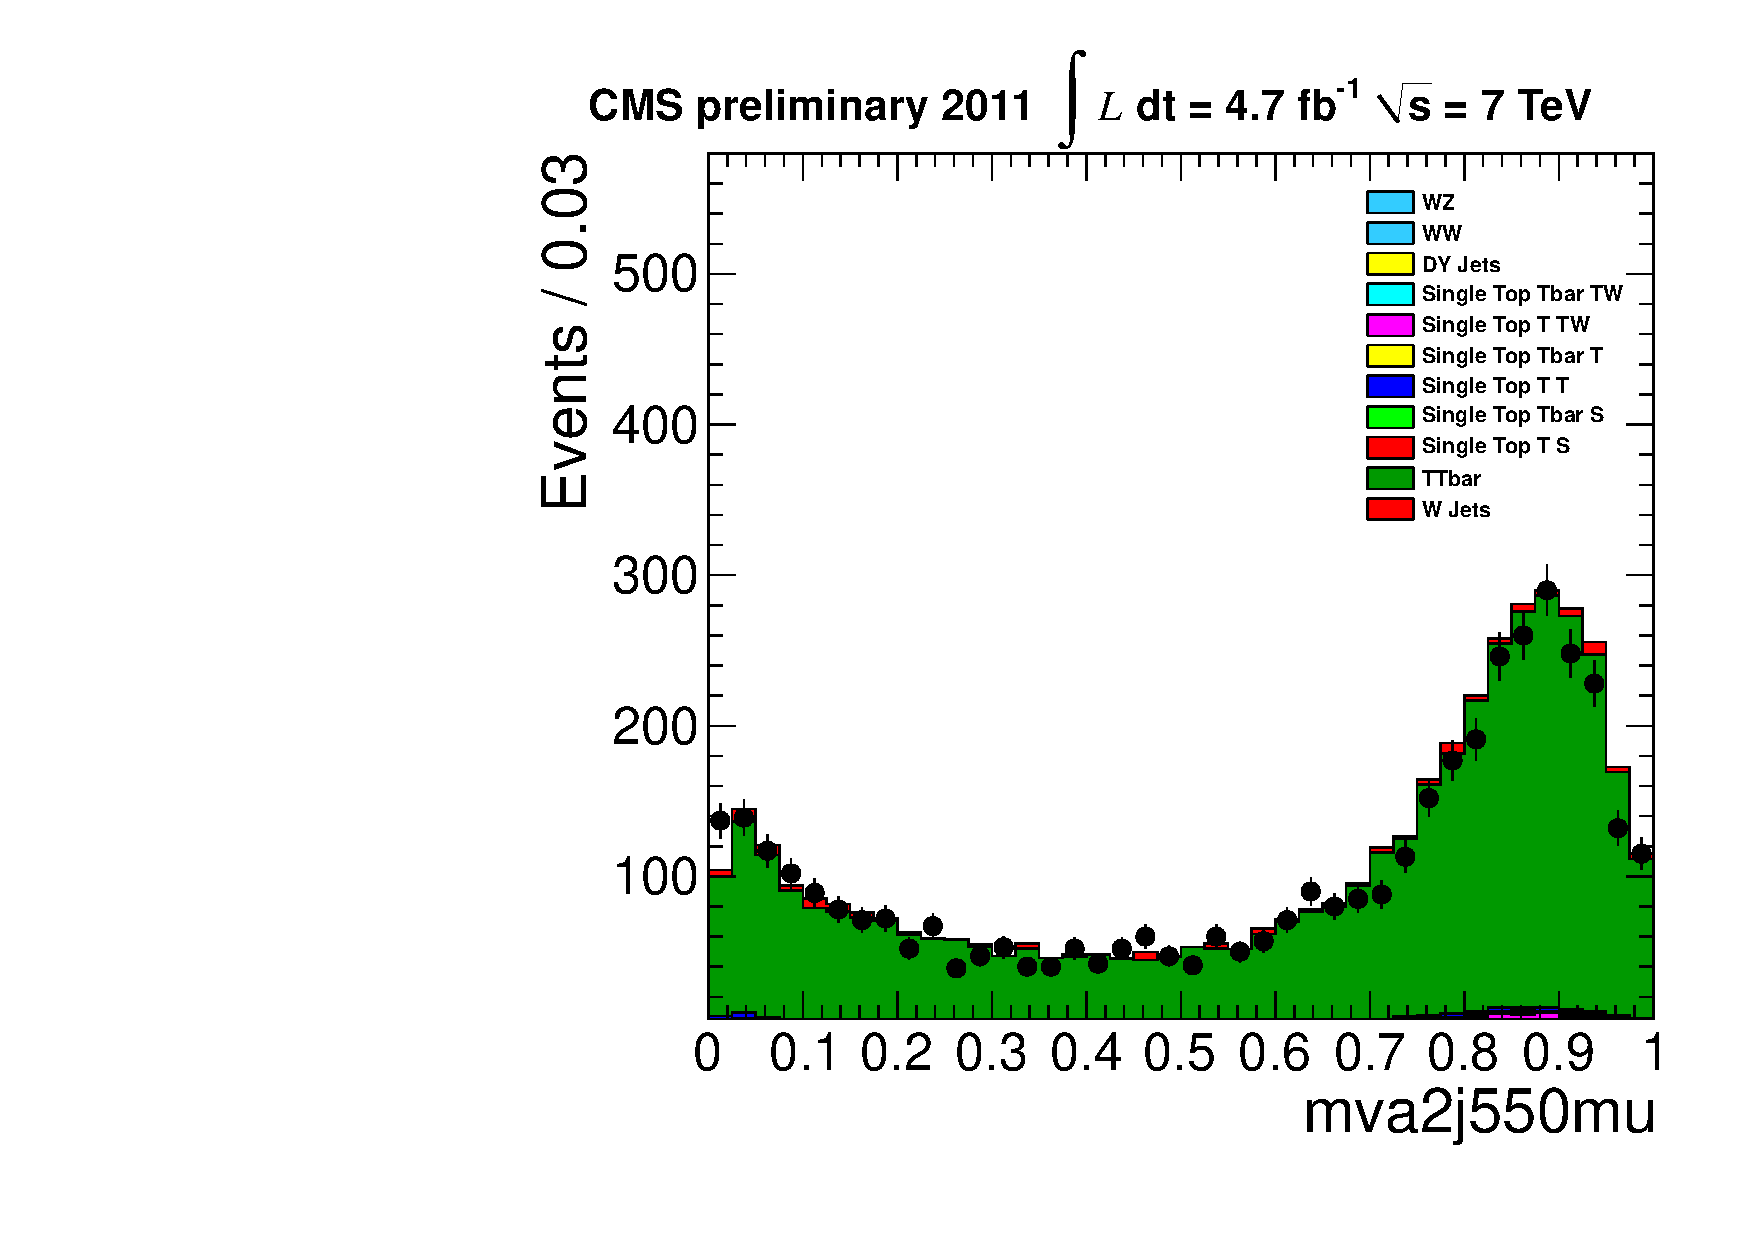
\includegraphics[width=0.49\textwidth]{figs/cl-mva2j550mu-inTTbar.pdf}
  \caption{\label{fig:mva:plots-mva2j550mu} The data-MC comparisons
    after standard event selection (left) and top pair
    selection (right) for the working point: mva2j550mu.}
\end{figure}

%%%%%%%%%%%%%%%%%%% mva2j600mu
\begin{figure}[!t]
  \centering
  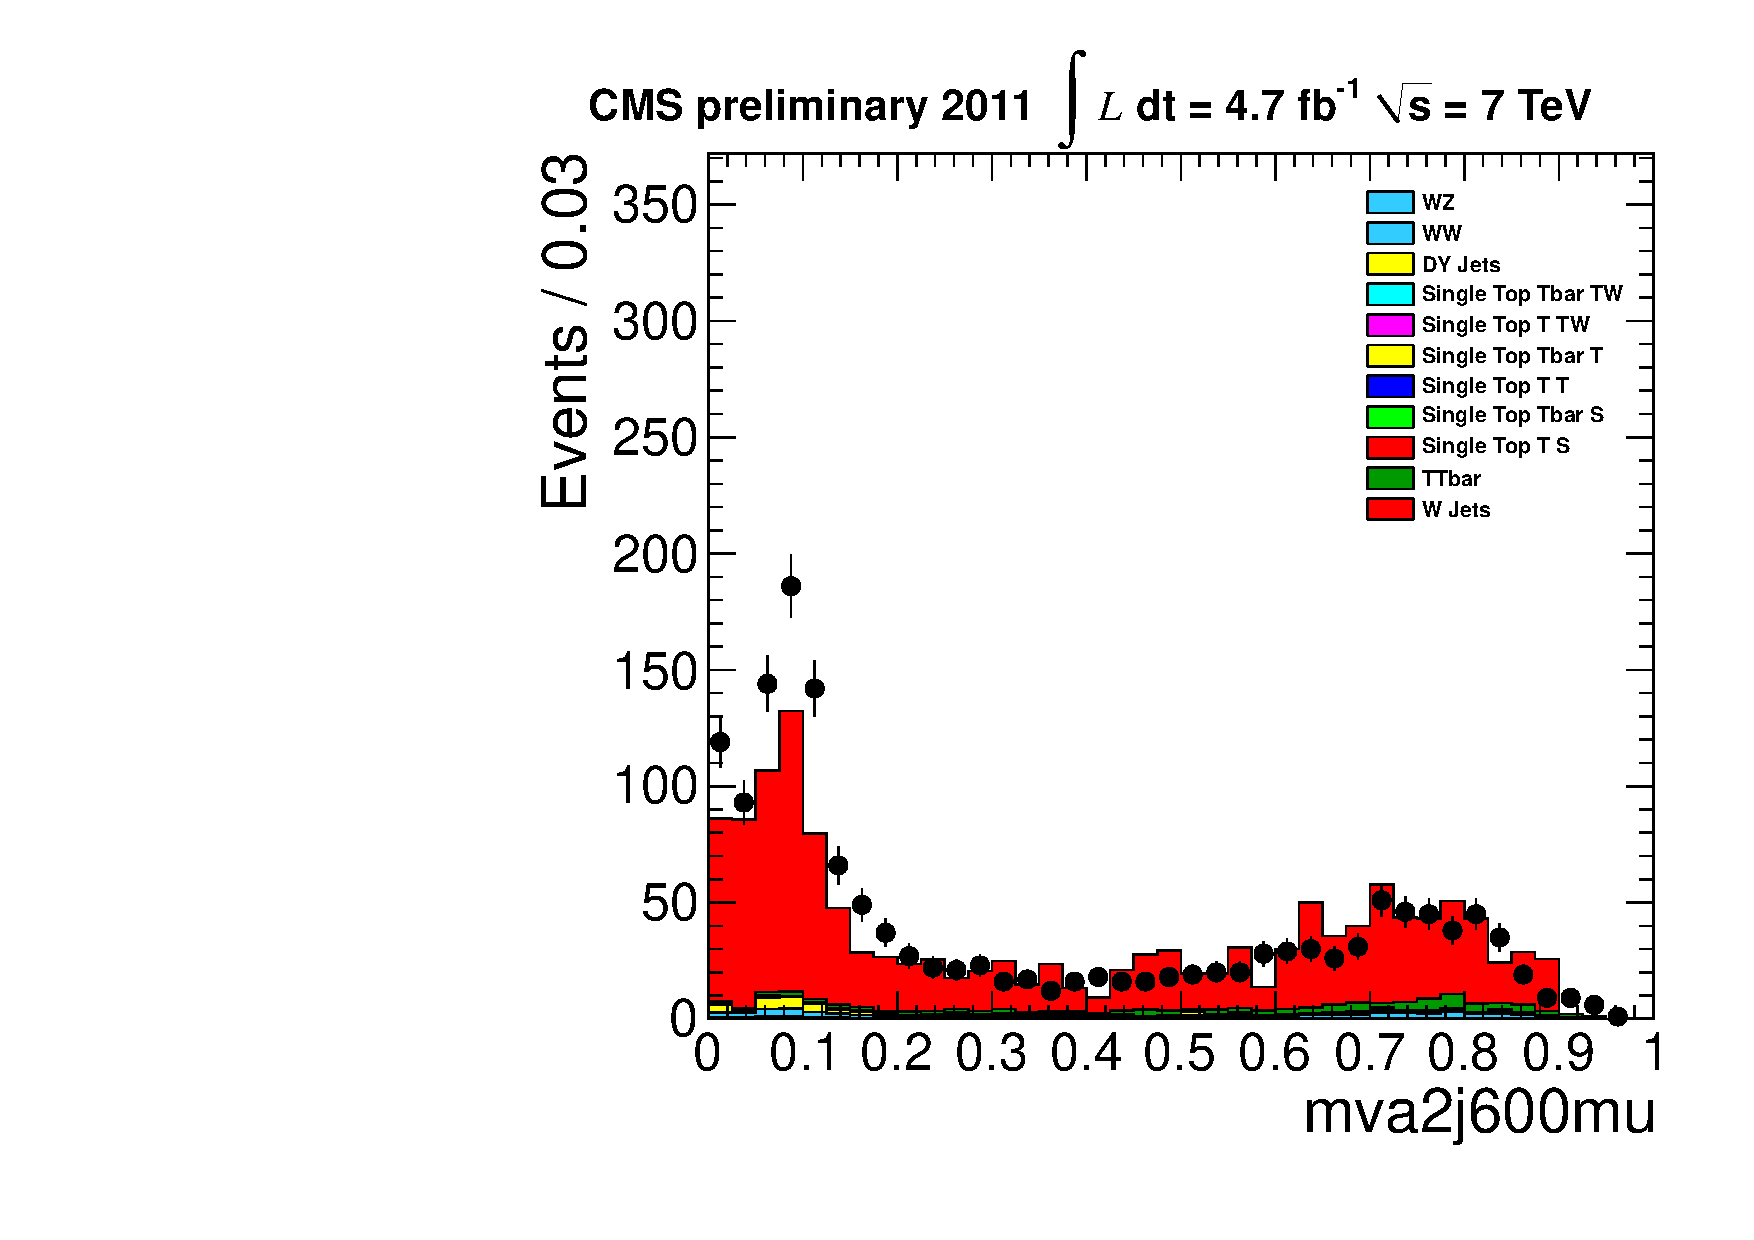
\includegraphics[width=0.49\textwidth]{figs/cl-mva2j600mu-normal.pdf}
  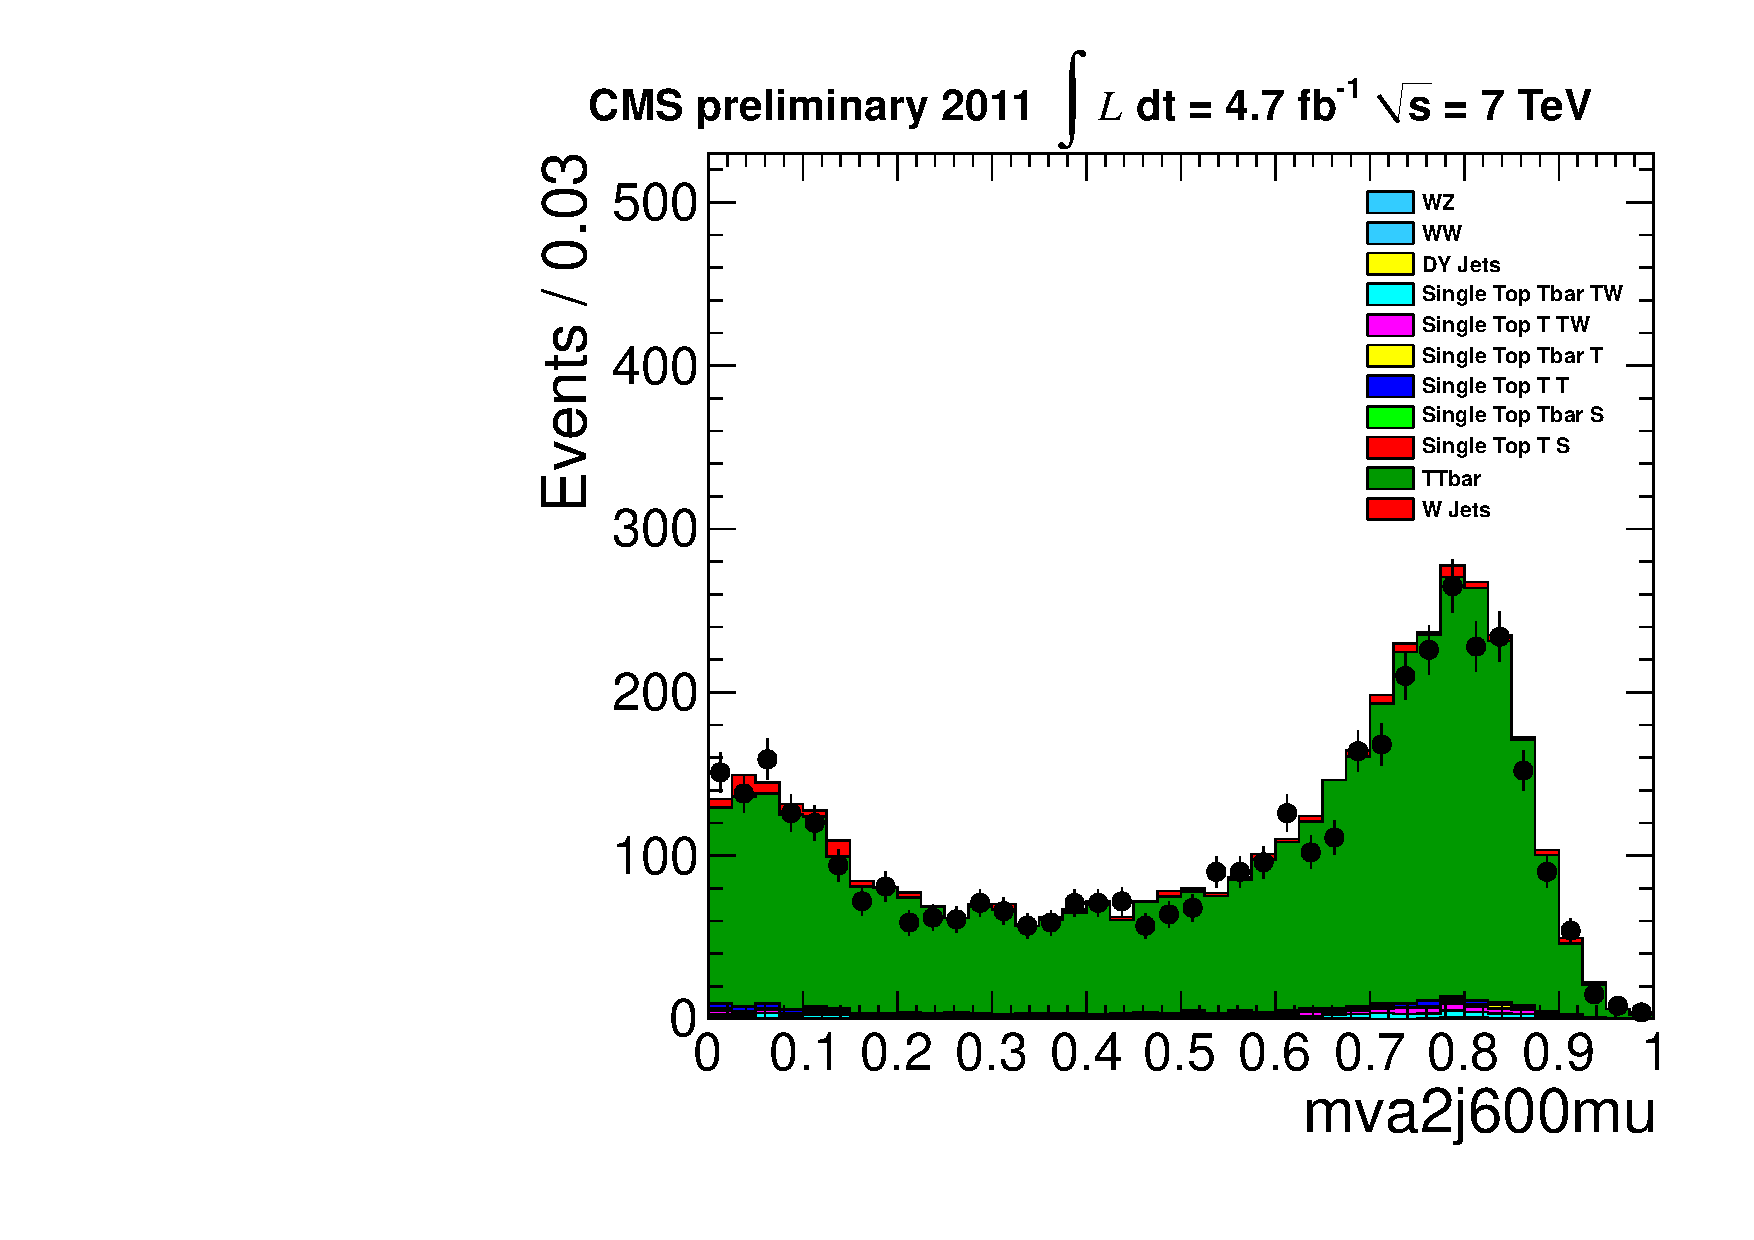
\includegraphics[width=0.49\textwidth]{figs/cl-mva2j600mu-inTTbar.pdf}
  \caption{\label{fig:mva:plots-mva2j600mu} The data-MC comparisons
    after standard event selection (left) and top pair
    selection (right) for the working point: mva2j600mu.}
\end{figure}

\clearpage
%%%%%%%%%%%%%%%%%%%%%%%%%%%%%%%%%%%%%%%%%%%%%%%%%%%%%%%%%%%%%%%%%%%%%%%%%%%%
%%%%%%%%%%%%%%%%%%% mva3j170mu
\begin{figure}[!t]
  \centering
  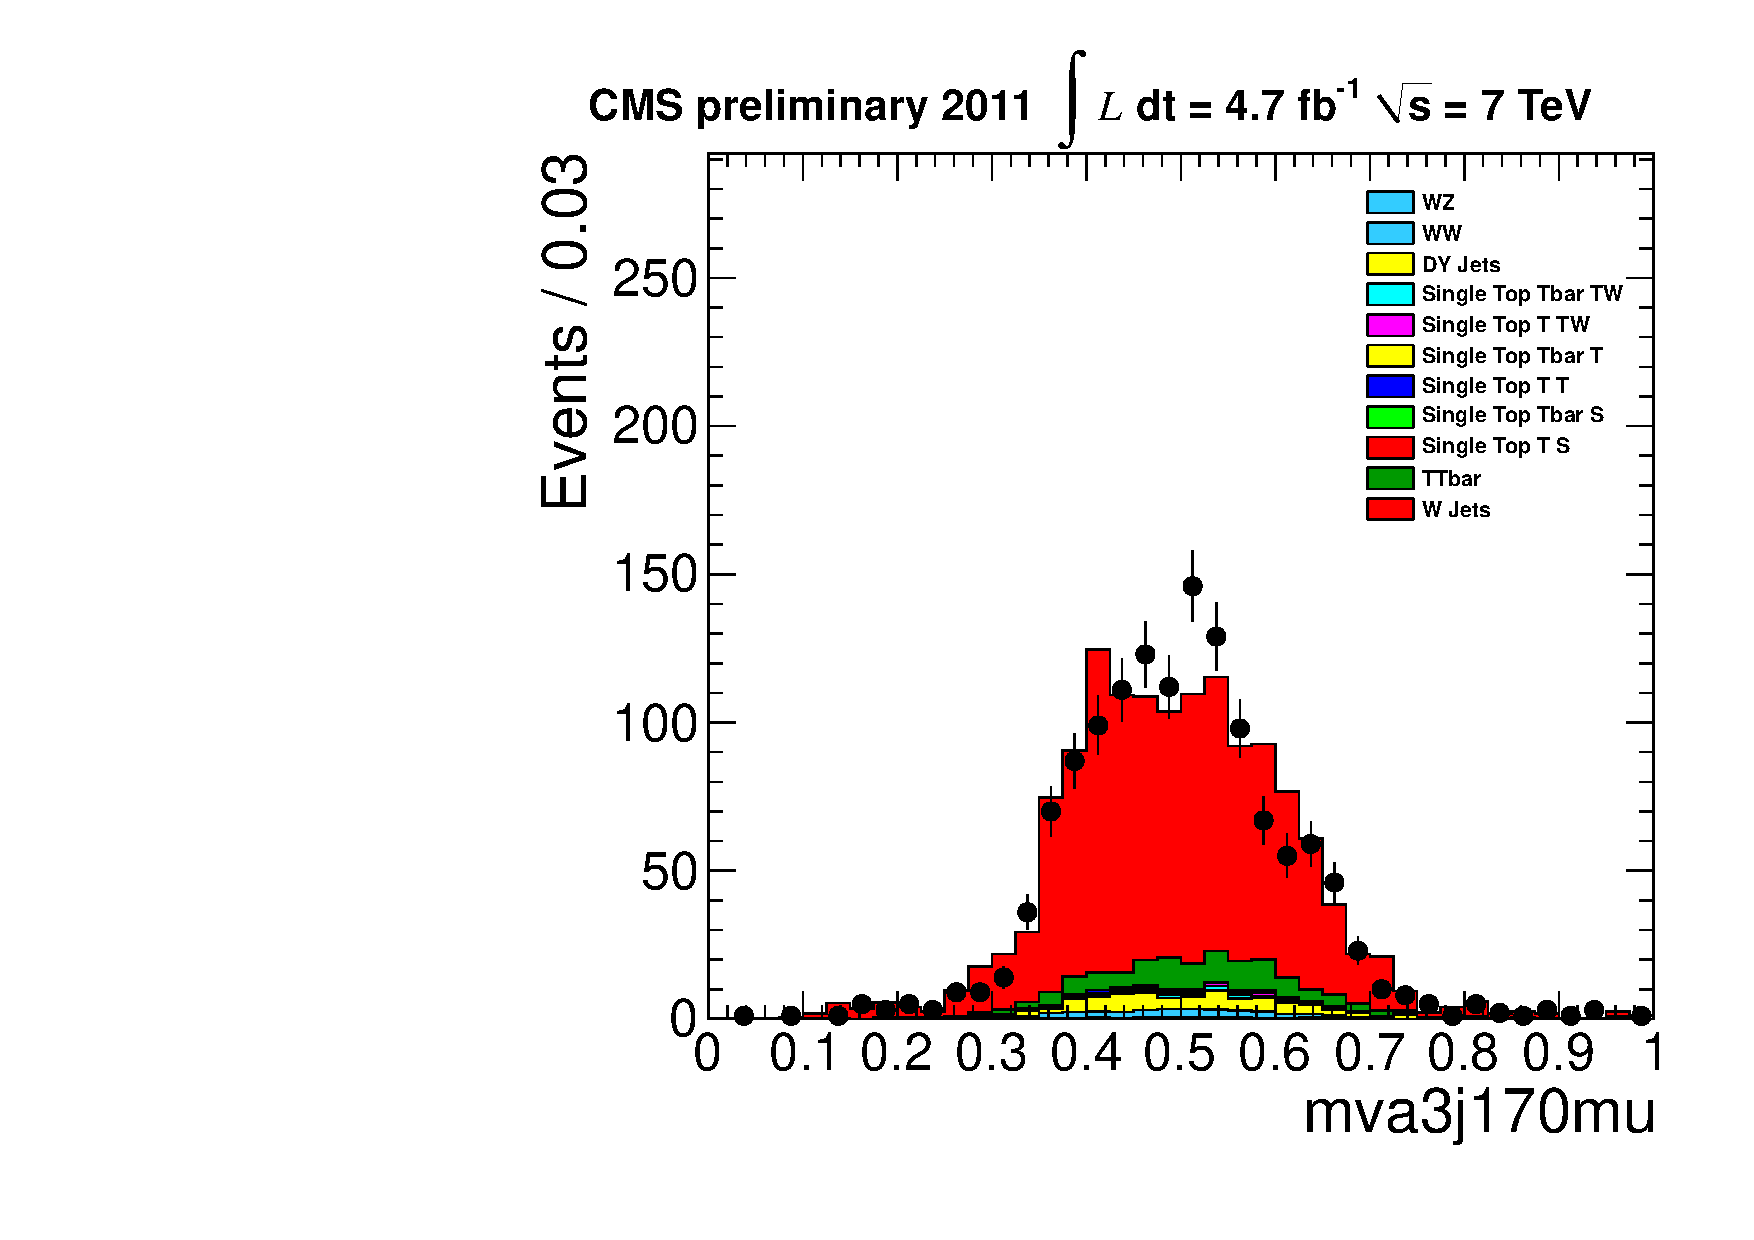
\includegraphics[width=0.49\textwidth]{figs/cl-mva3j170mu-normal.pdf}
  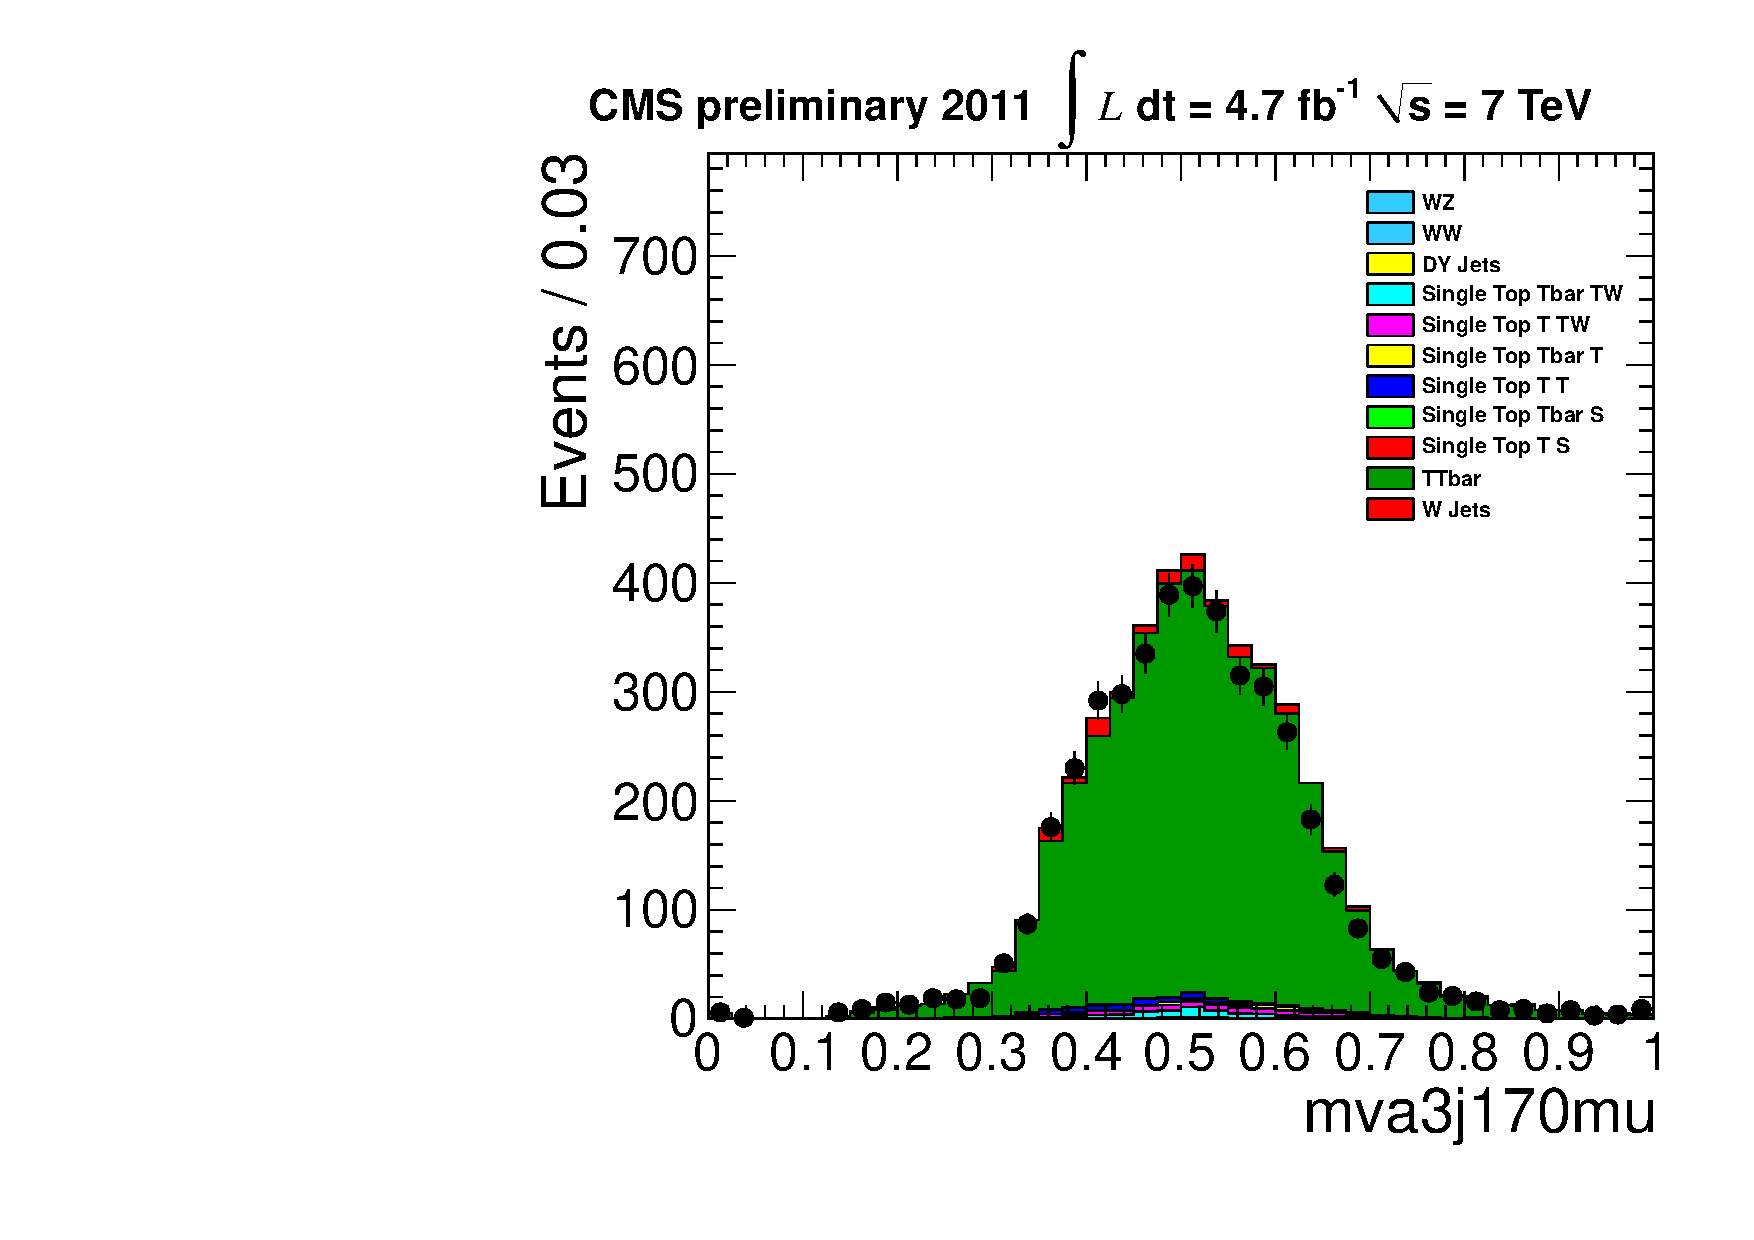
\includegraphics[width=0.49\textwidth]{figs/cl-mva3j170mu-inTTbar.pdf}
  \caption{\label{fig:mva:plots-mva3j170mu} The data-MC comparisons
    after standard event selection (left) and top pair
    selection (right) for the working point: mva3j170mu.}
\end{figure}

%%%%%%%%%%%%%%%%%%% mva3j180mu
\begin{figure}[!t]
  \centering
  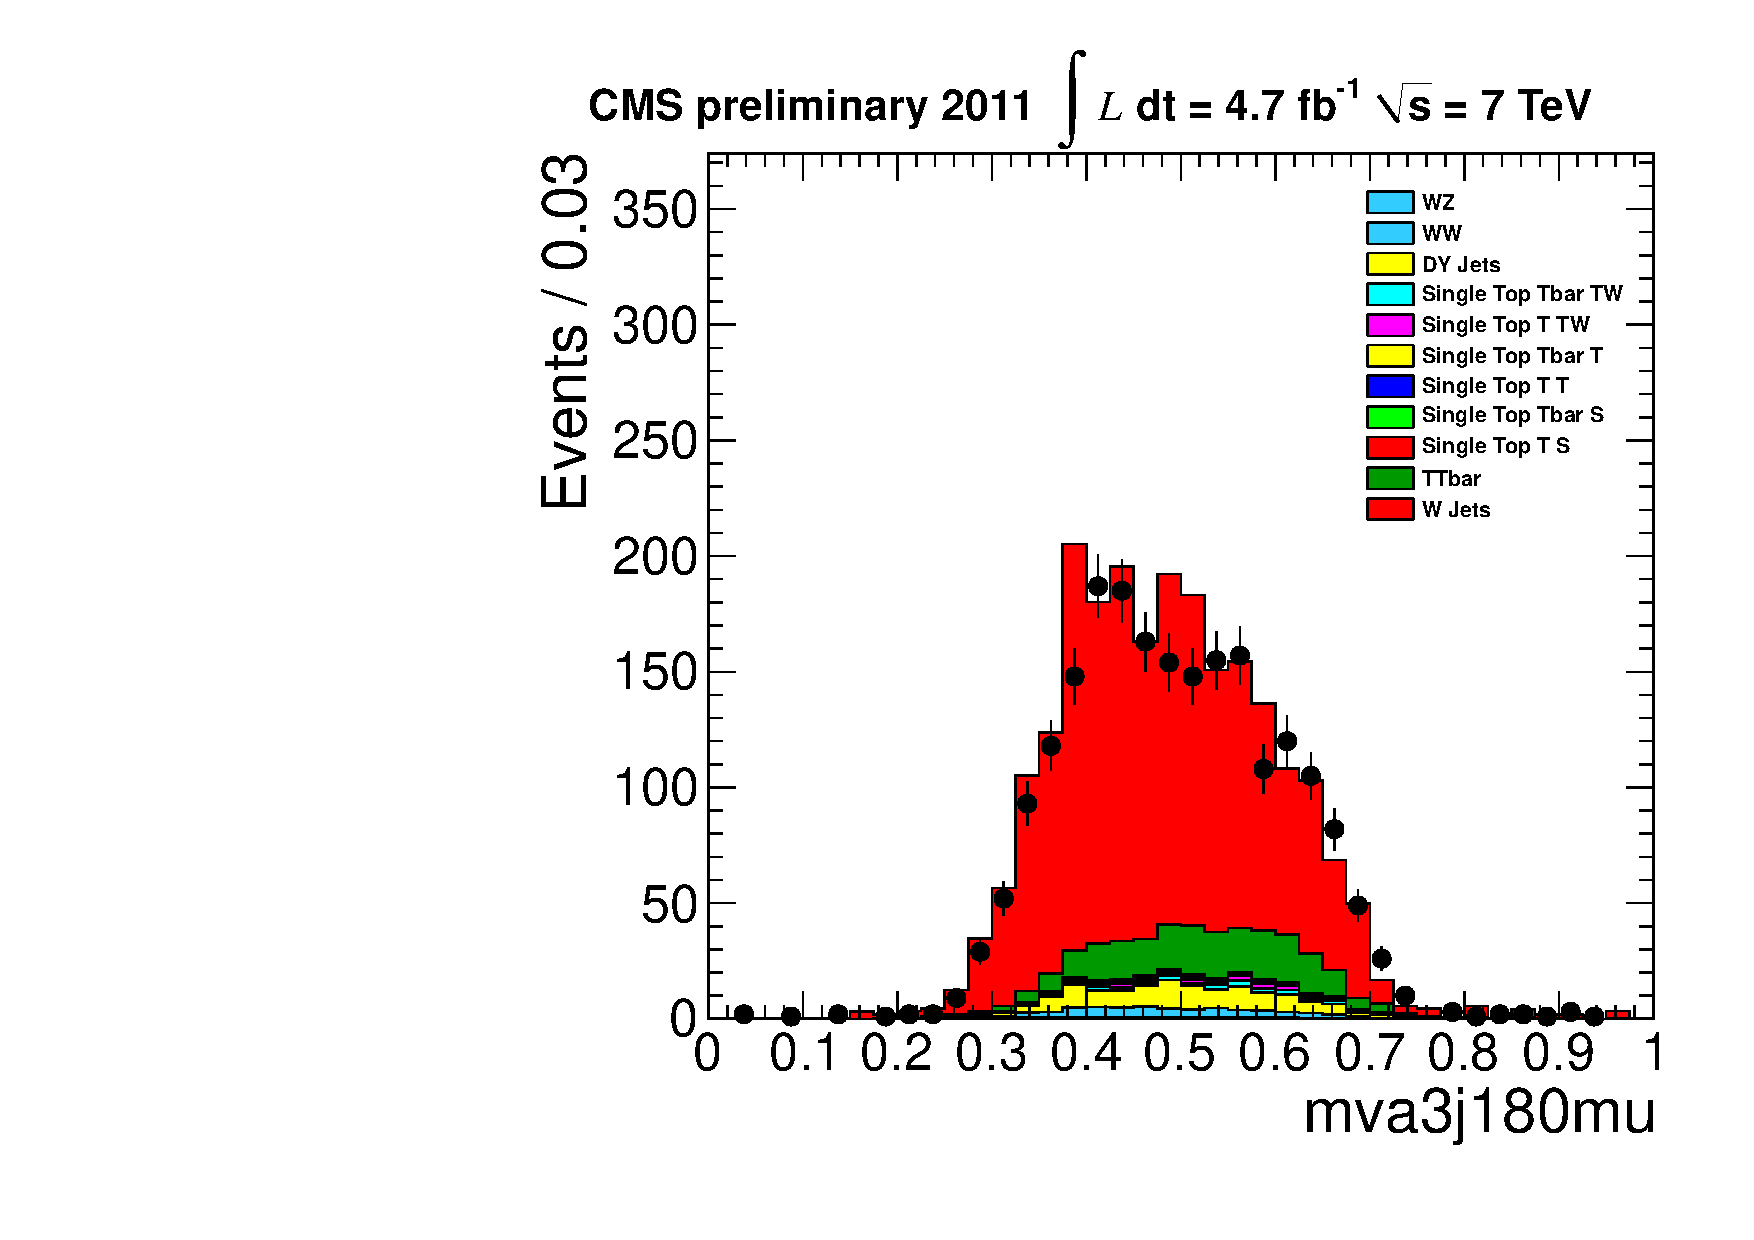
\includegraphics[width=0.49\textwidth]{figs/cl-mva3j180mu-normal.pdf}
  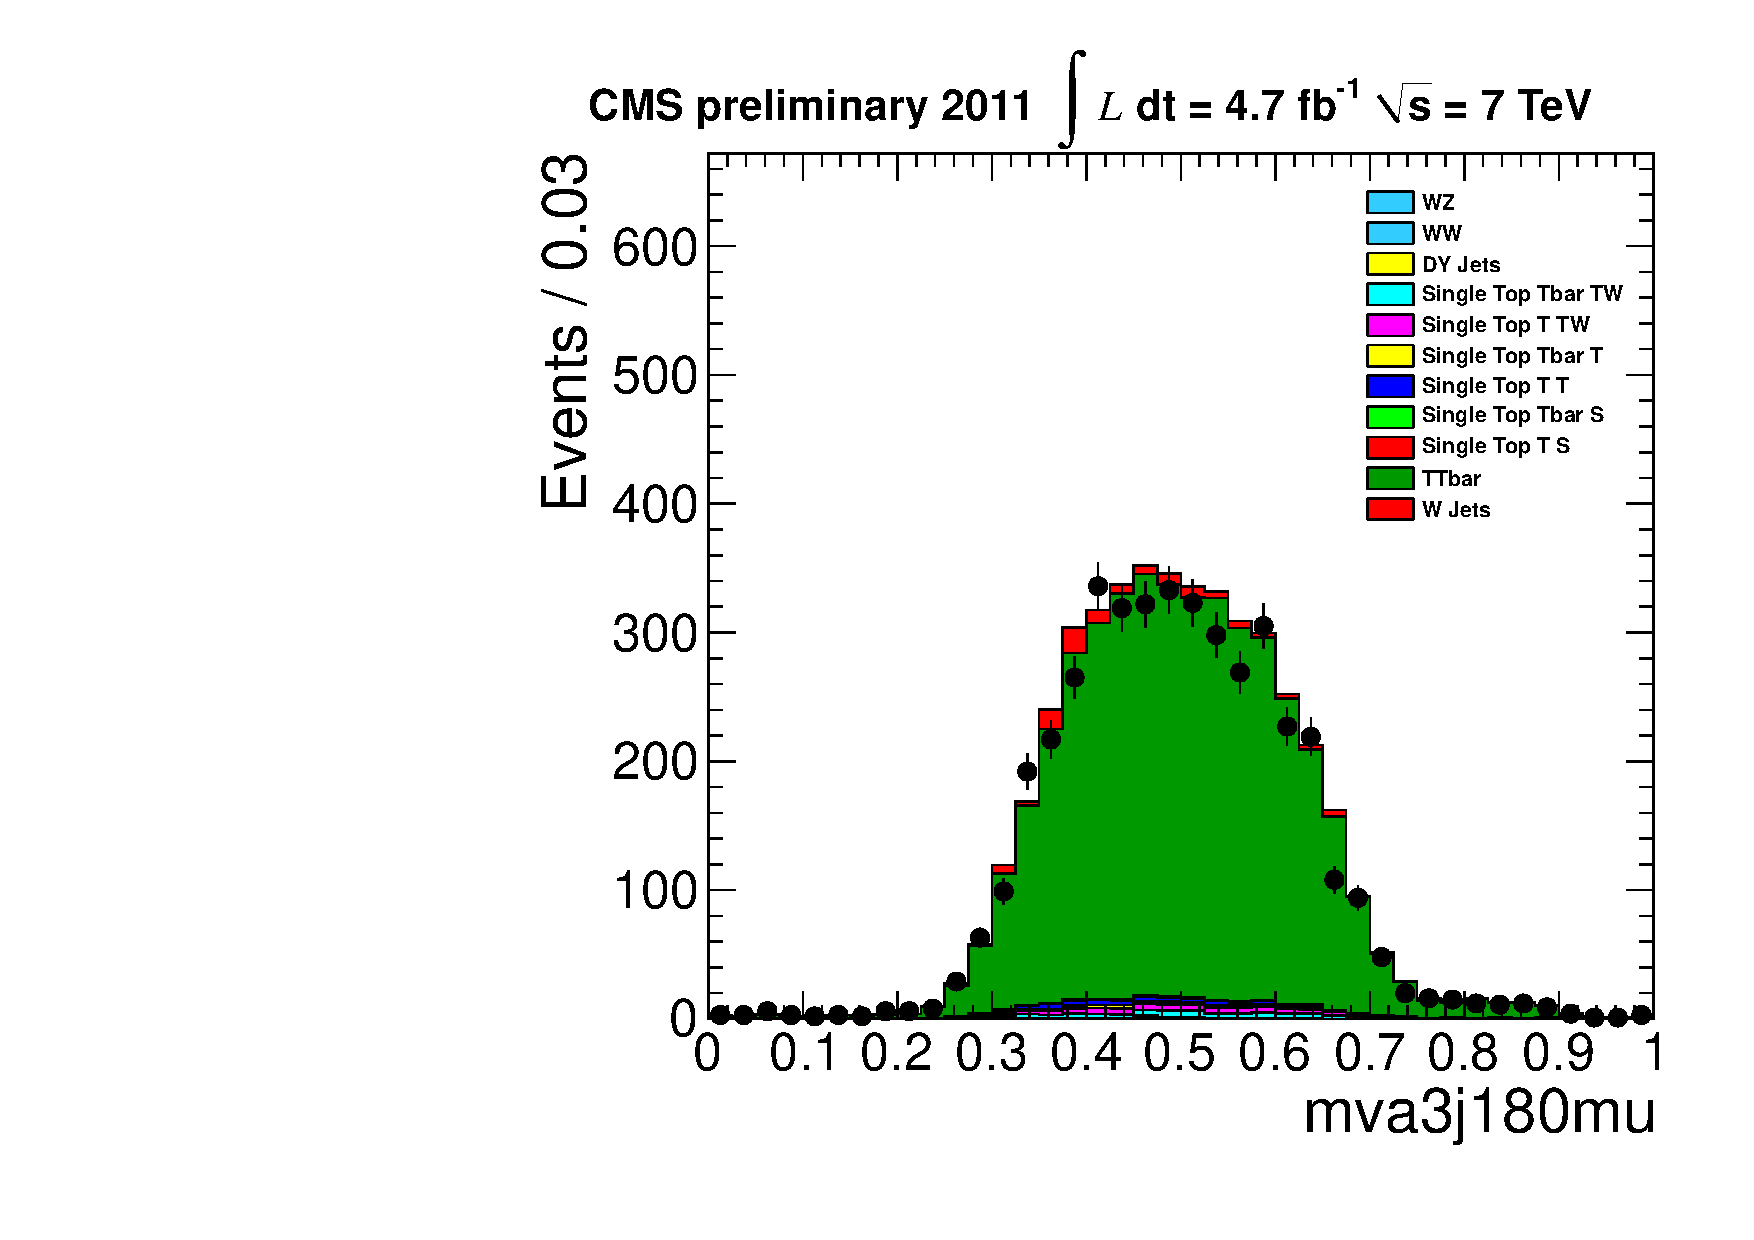
\includegraphics[width=0.49\textwidth]{figs/cl-mva3j180mu-inTTbar.pdf}
  \caption{\label{fig:mva:plots-mva3j180mu} The data-MC comparisons
    after standard event selection (left) and top pair
    selection (right) for the working point: mva3j180mu.}
\end{figure}

%%%%%%%%%%%%%%%%%%% mva3j190mu
\begin{figure}[!t]
  \centering
  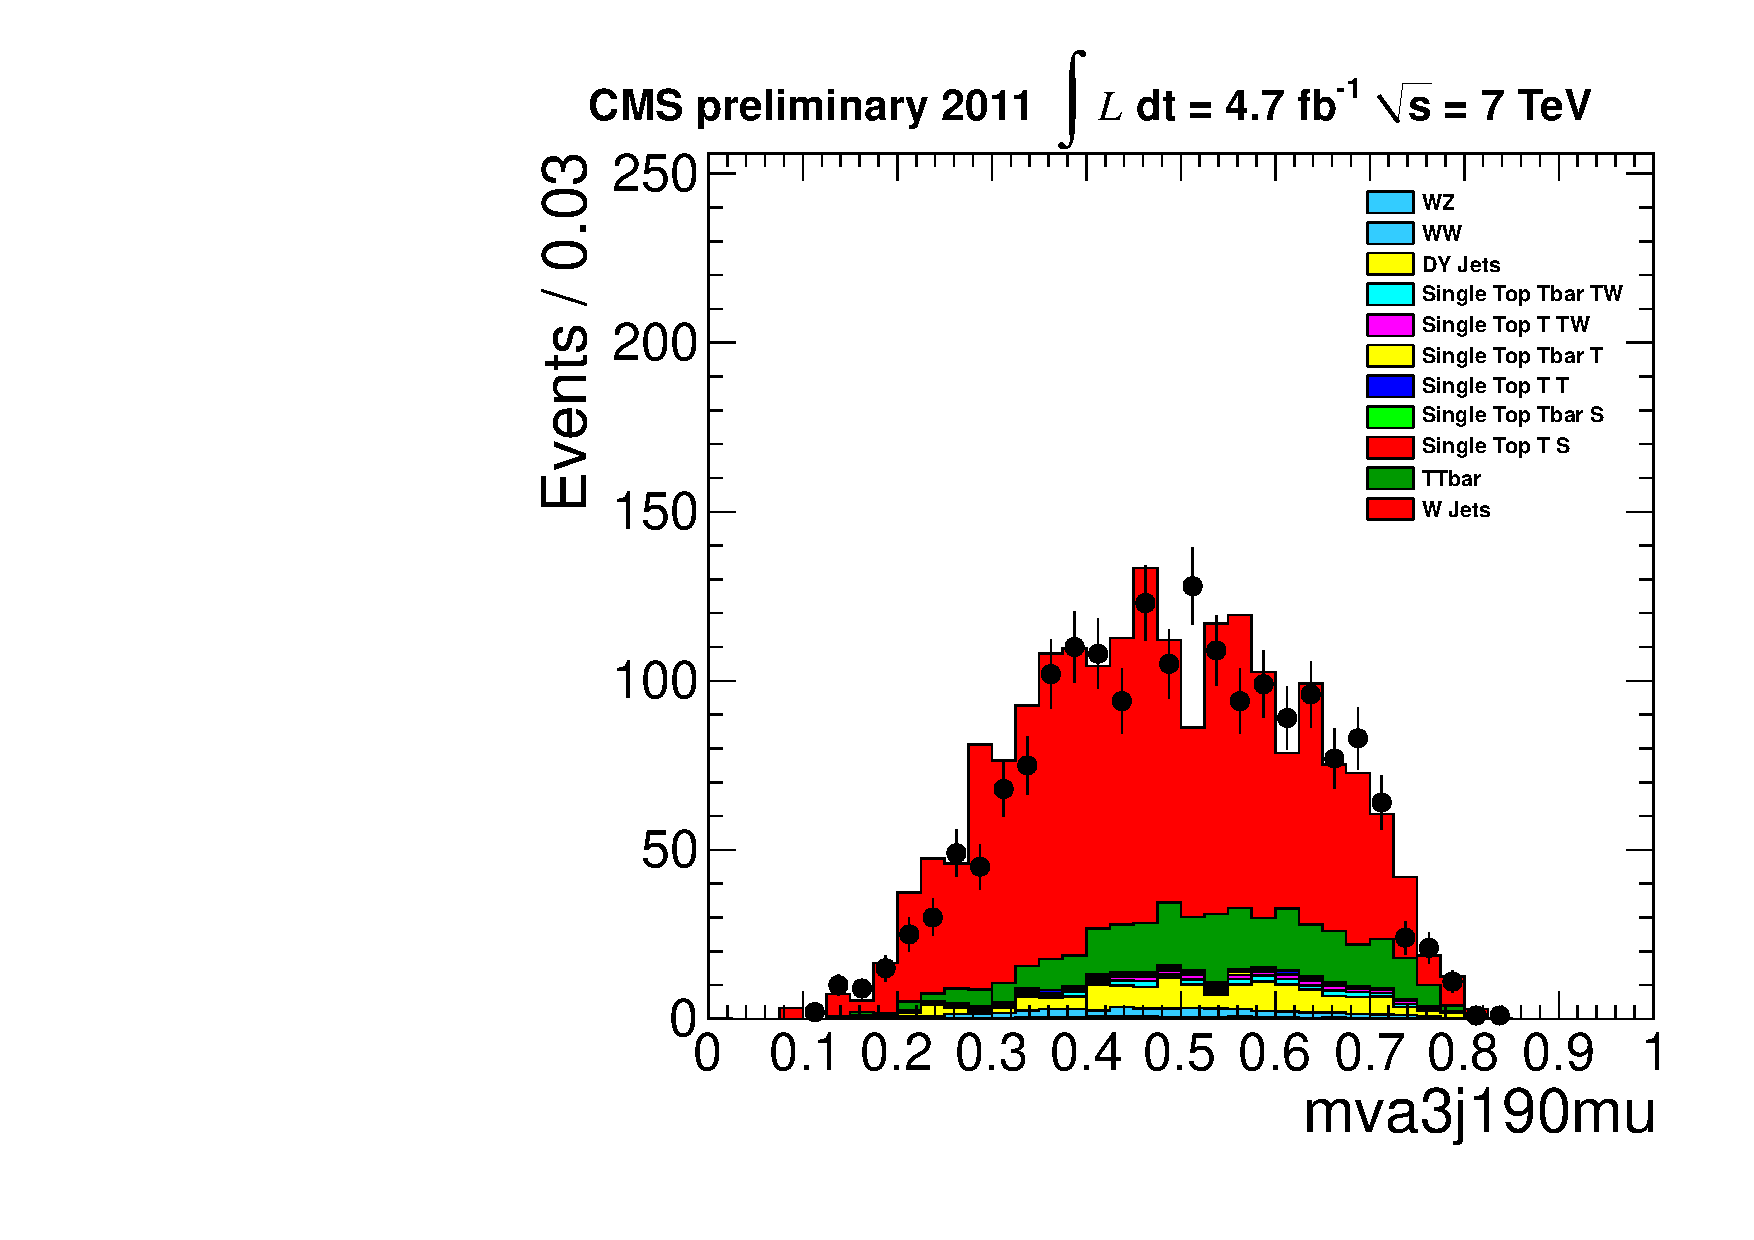
\includegraphics[width=0.49\textwidth]{figs/cl-mva3j190mu-normal.pdf}
  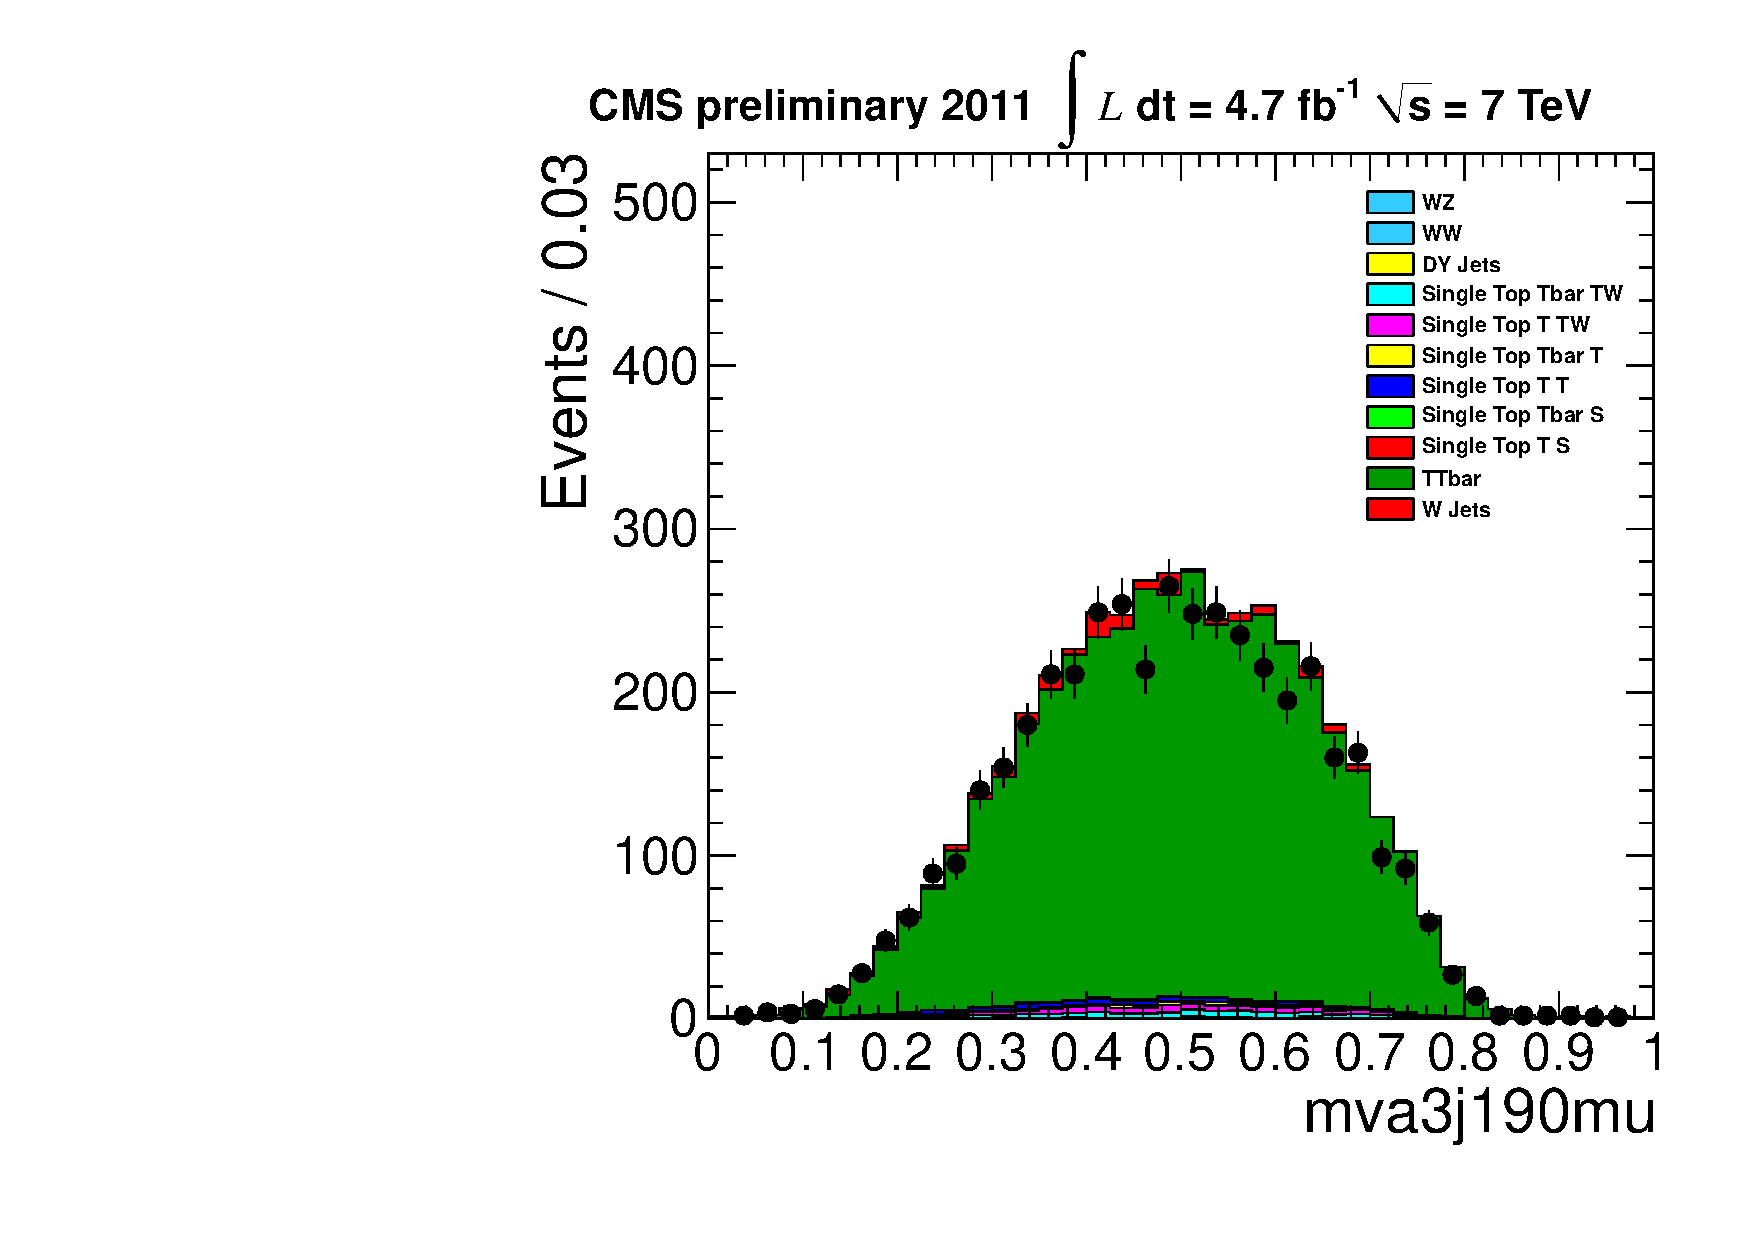
\includegraphics[width=0.49\textwidth]{figs/cl-mva3j190mu-inTTbar.pdf}
  \caption{\label{fig:mva:plots-mva3j190mu} The data-MC comparisons
    after standard event selection (left) and top pair
    selection (right) for the working point: mva3j190mu.}
\end{figure}

%%%%%%%%%%%%%%%%%%% mva3j200mu
\begin{figure}[!t]
  \centering
  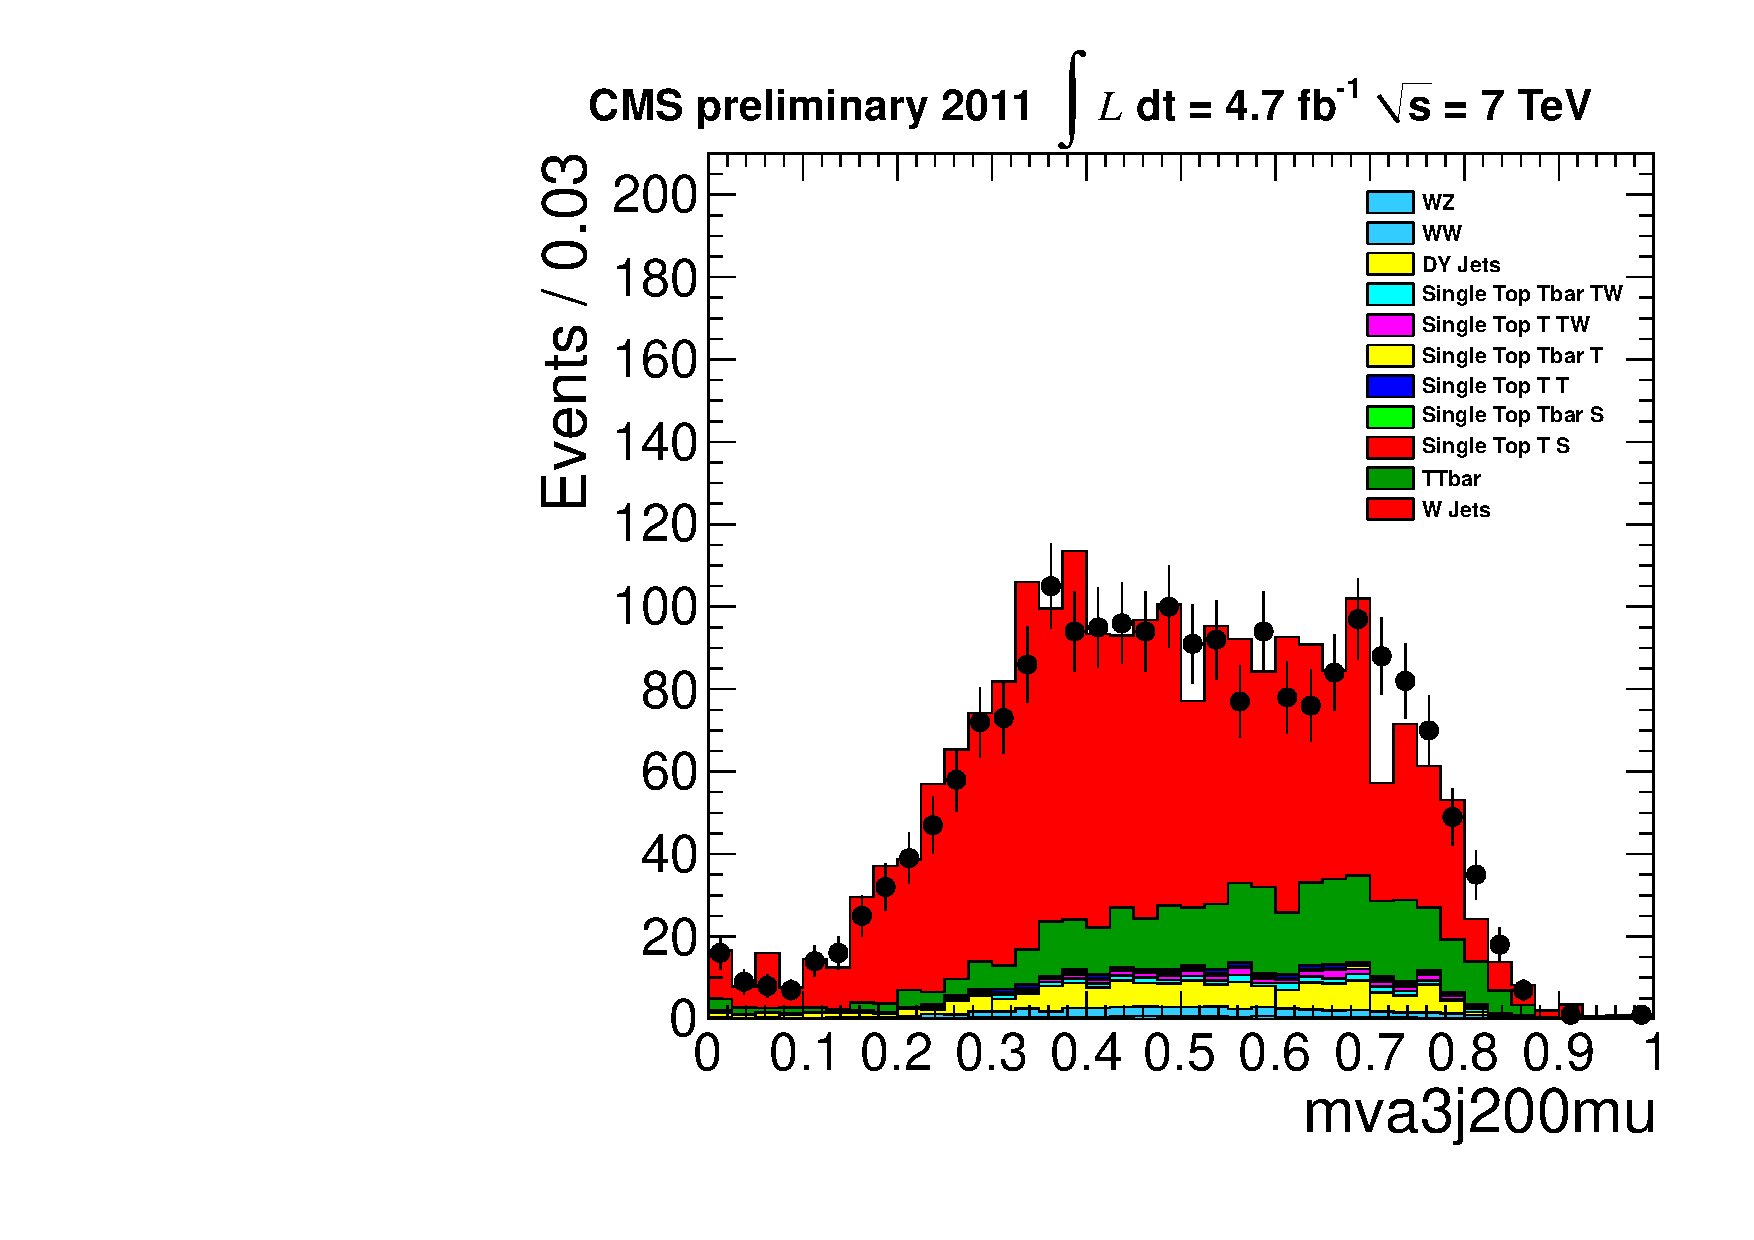
\includegraphics[width=0.49\textwidth]{figs/cl-mva3j200mu-normal.pdf}
  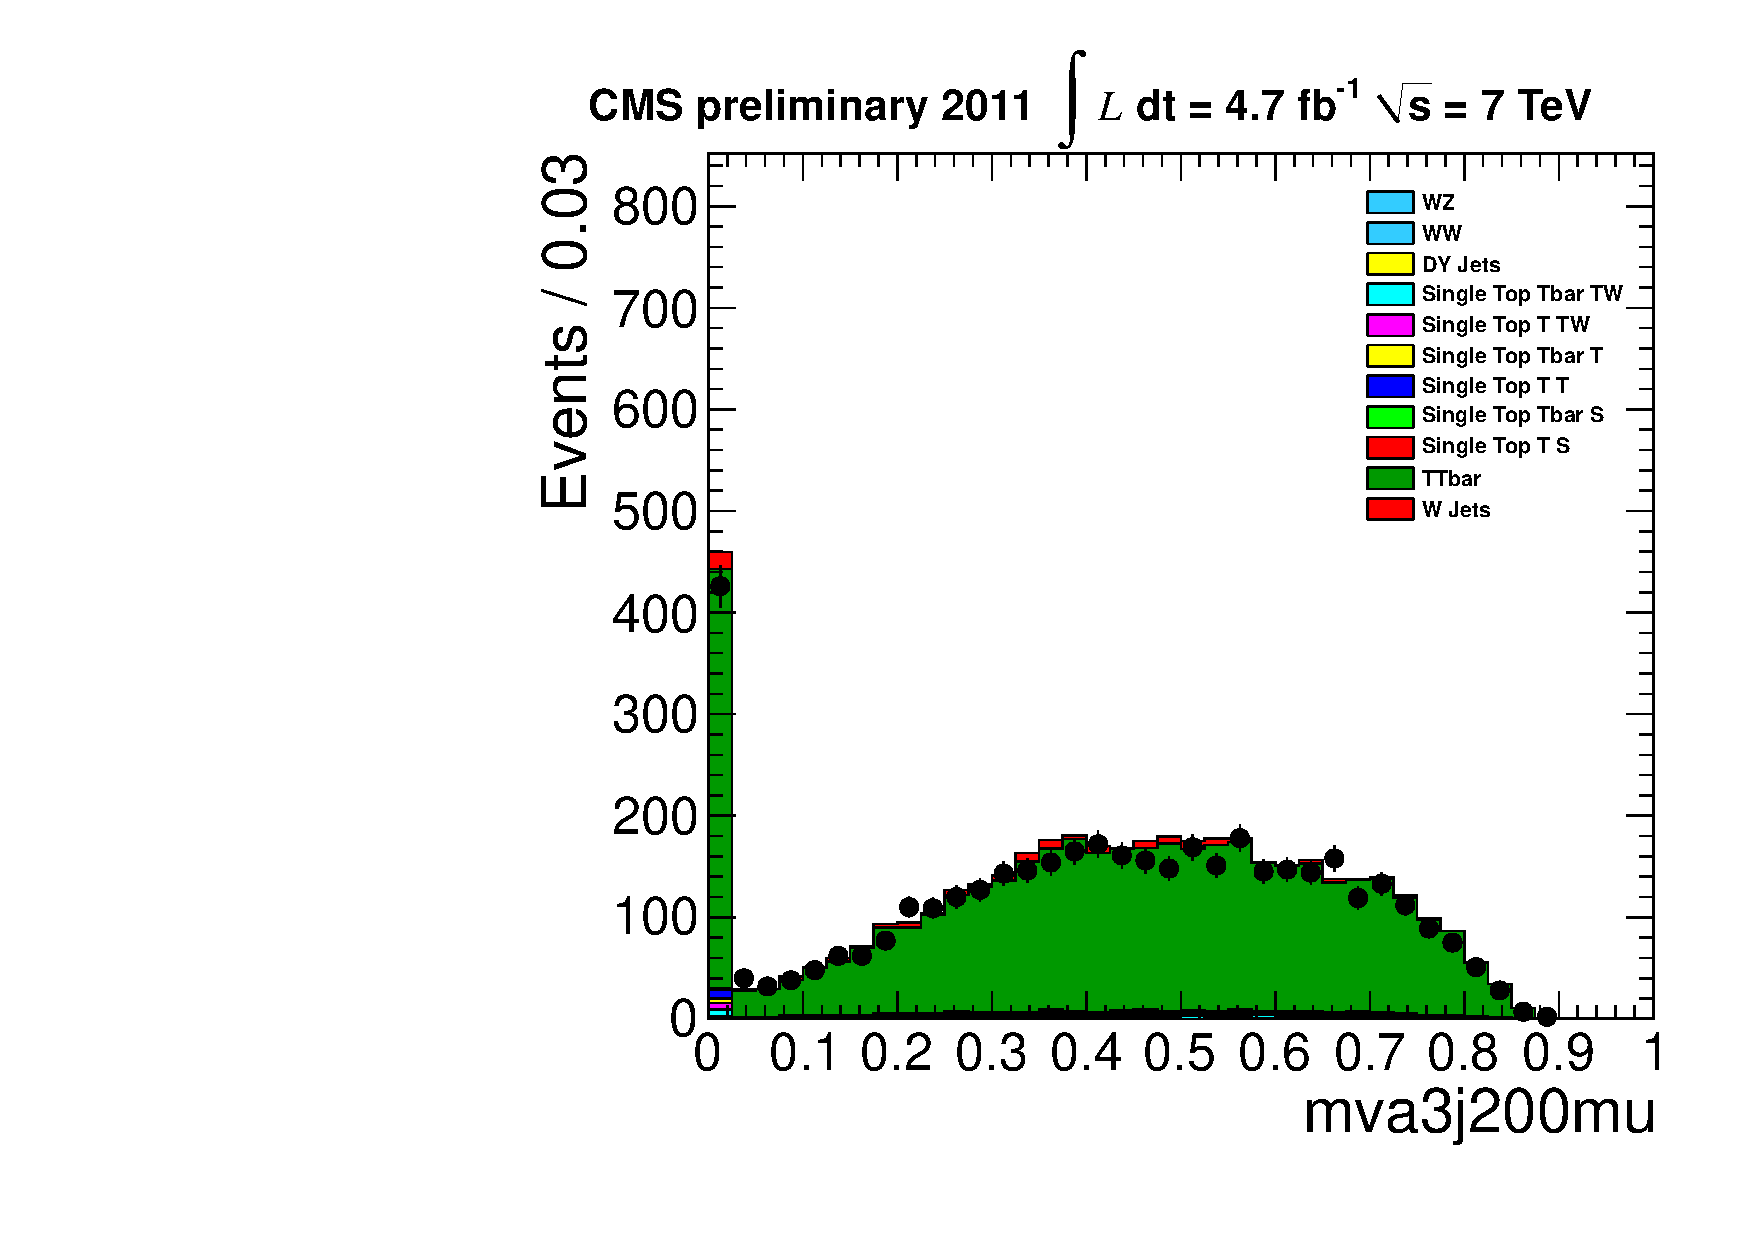
\includegraphics[width=0.49\textwidth]{figs/cl-mva3j200mu-inTTbar.pdf}
  \caption{\label{fig:mva:plots-mva3j200mu} The data-MC comparisons
    after standard event selection (left) and top pair
    selection (right) for the working point: mva3j200mu.}
\end{figure}

%%%%%%%%%%%%%%%%%%% mva3j250mu
\begin{figure}[!t]
  \centering
  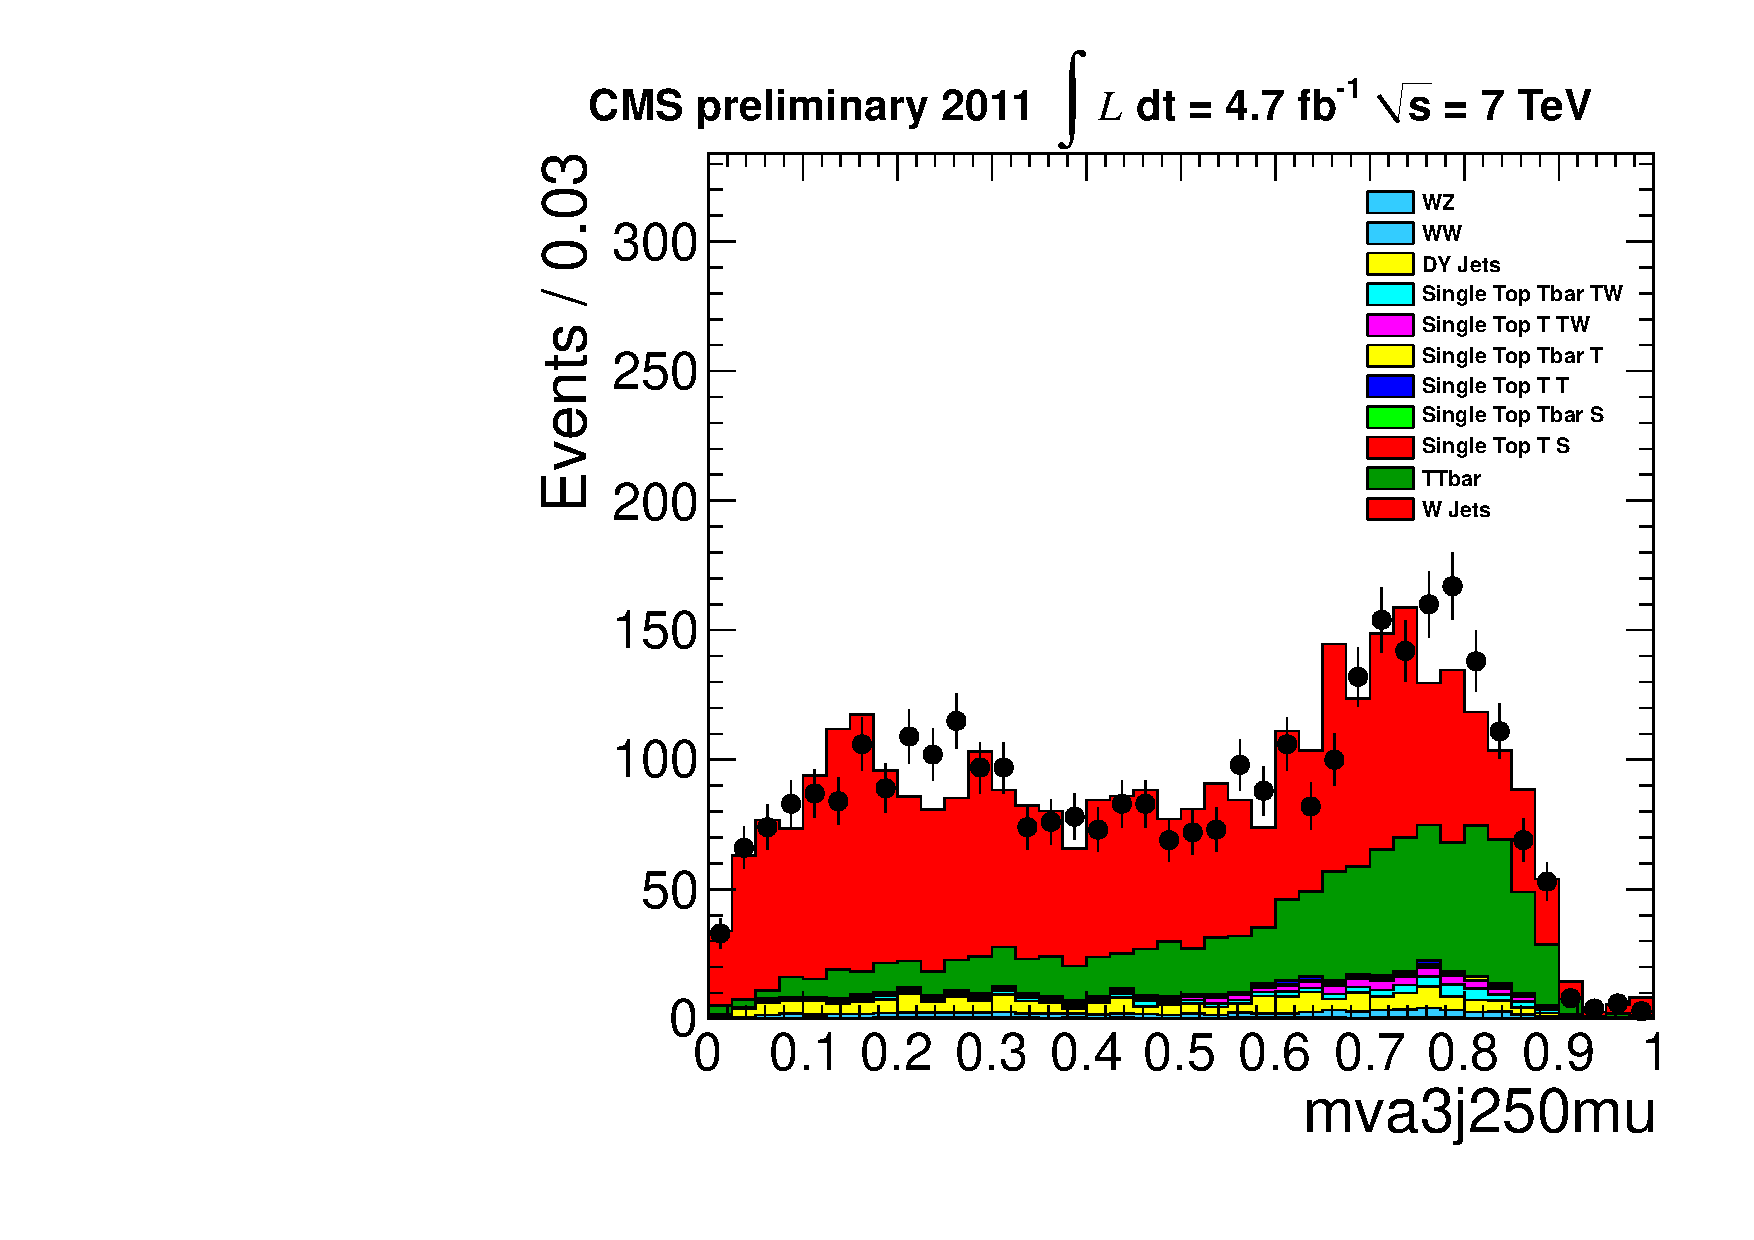
\includegraphics[width=0.49\textwidth]{figs/cl-mva3j250mu-normal.pdf}
  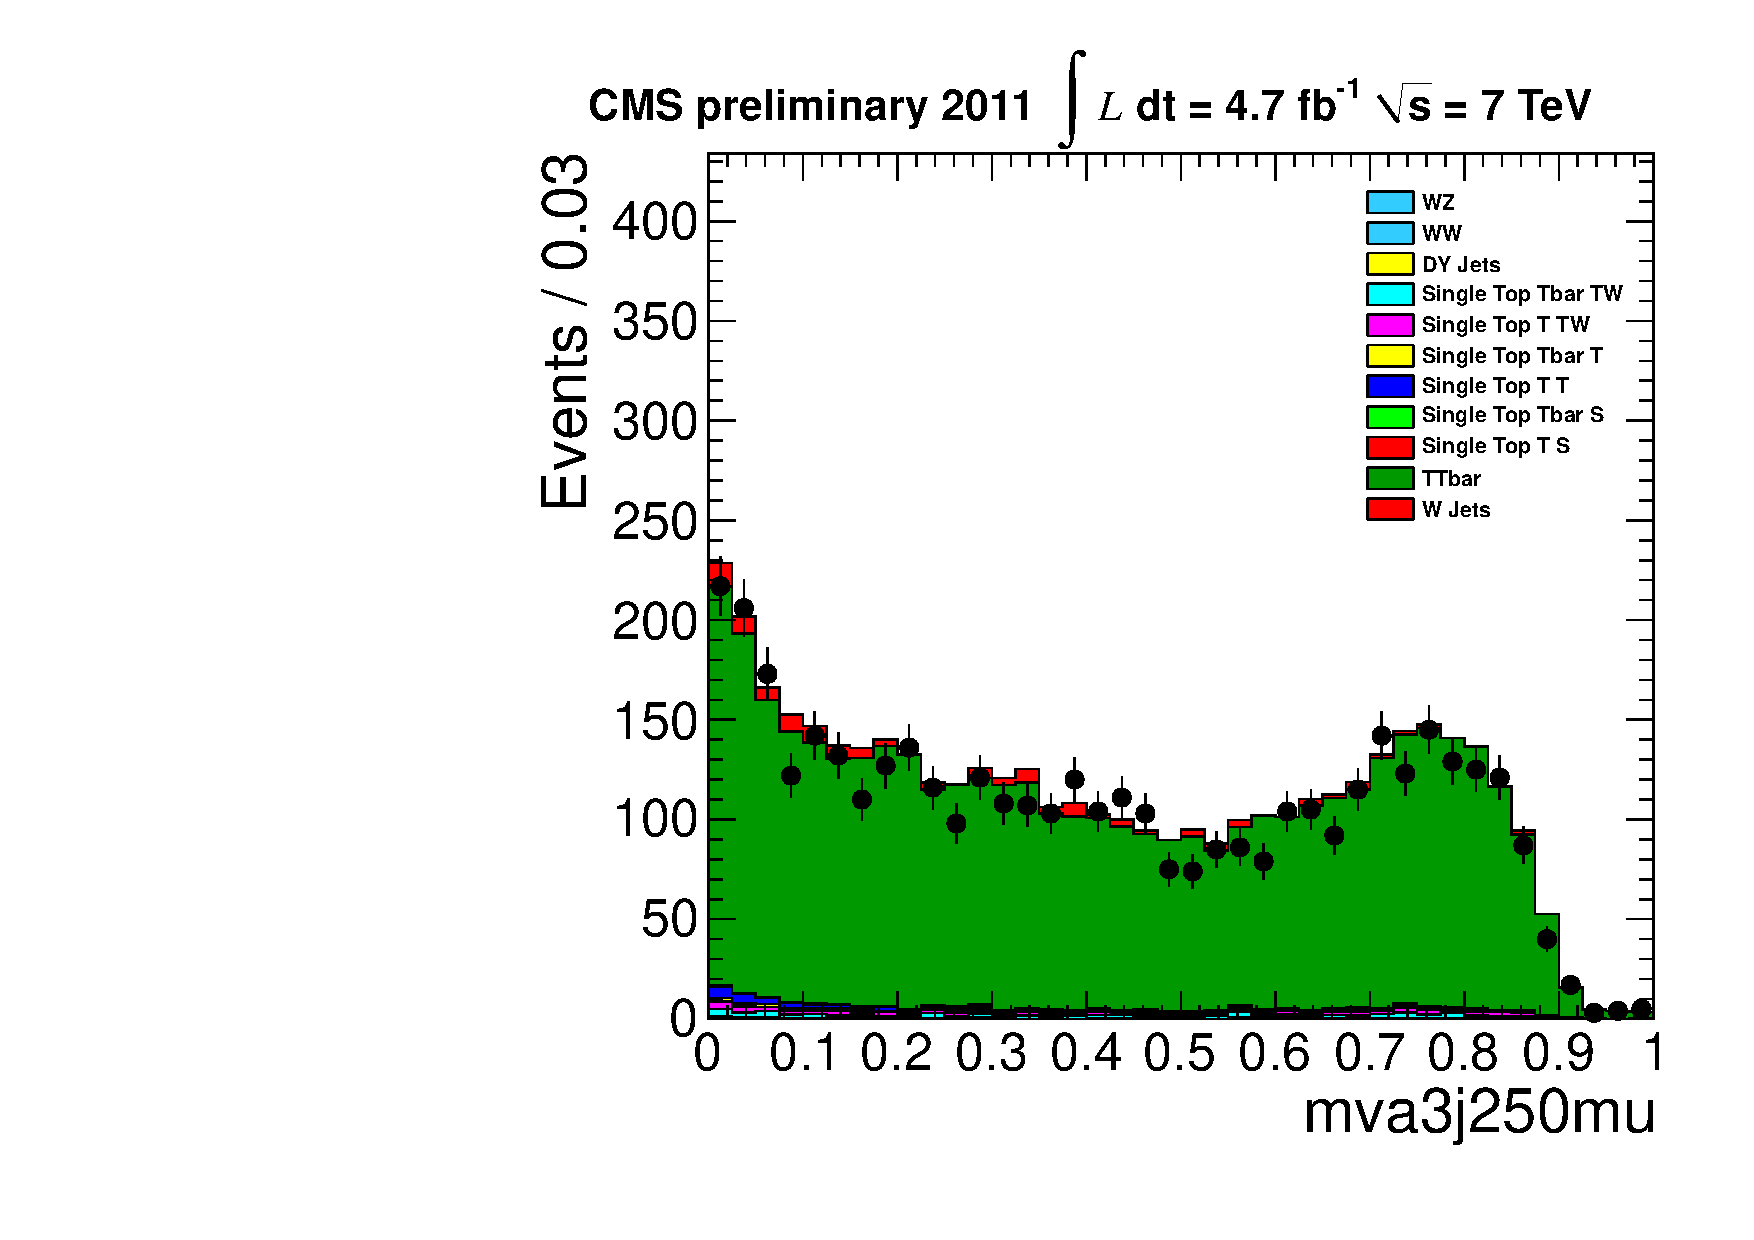
\includegraphics[width=0.49\textwidth]{figs/cl-mva3j250mu-inTTbar.pdf}
  \caption{\label{fig:mva:plots-mva3j250mu} The data-MC comparisons
    after standard event selection (left) and top pair
    selection (right) for the working point: mva3j250mu.}
\end{figure}

%%%%%%%%%%%%%%%%%%% mva3j300mu
\begin{figure}[!t]
  \centering
  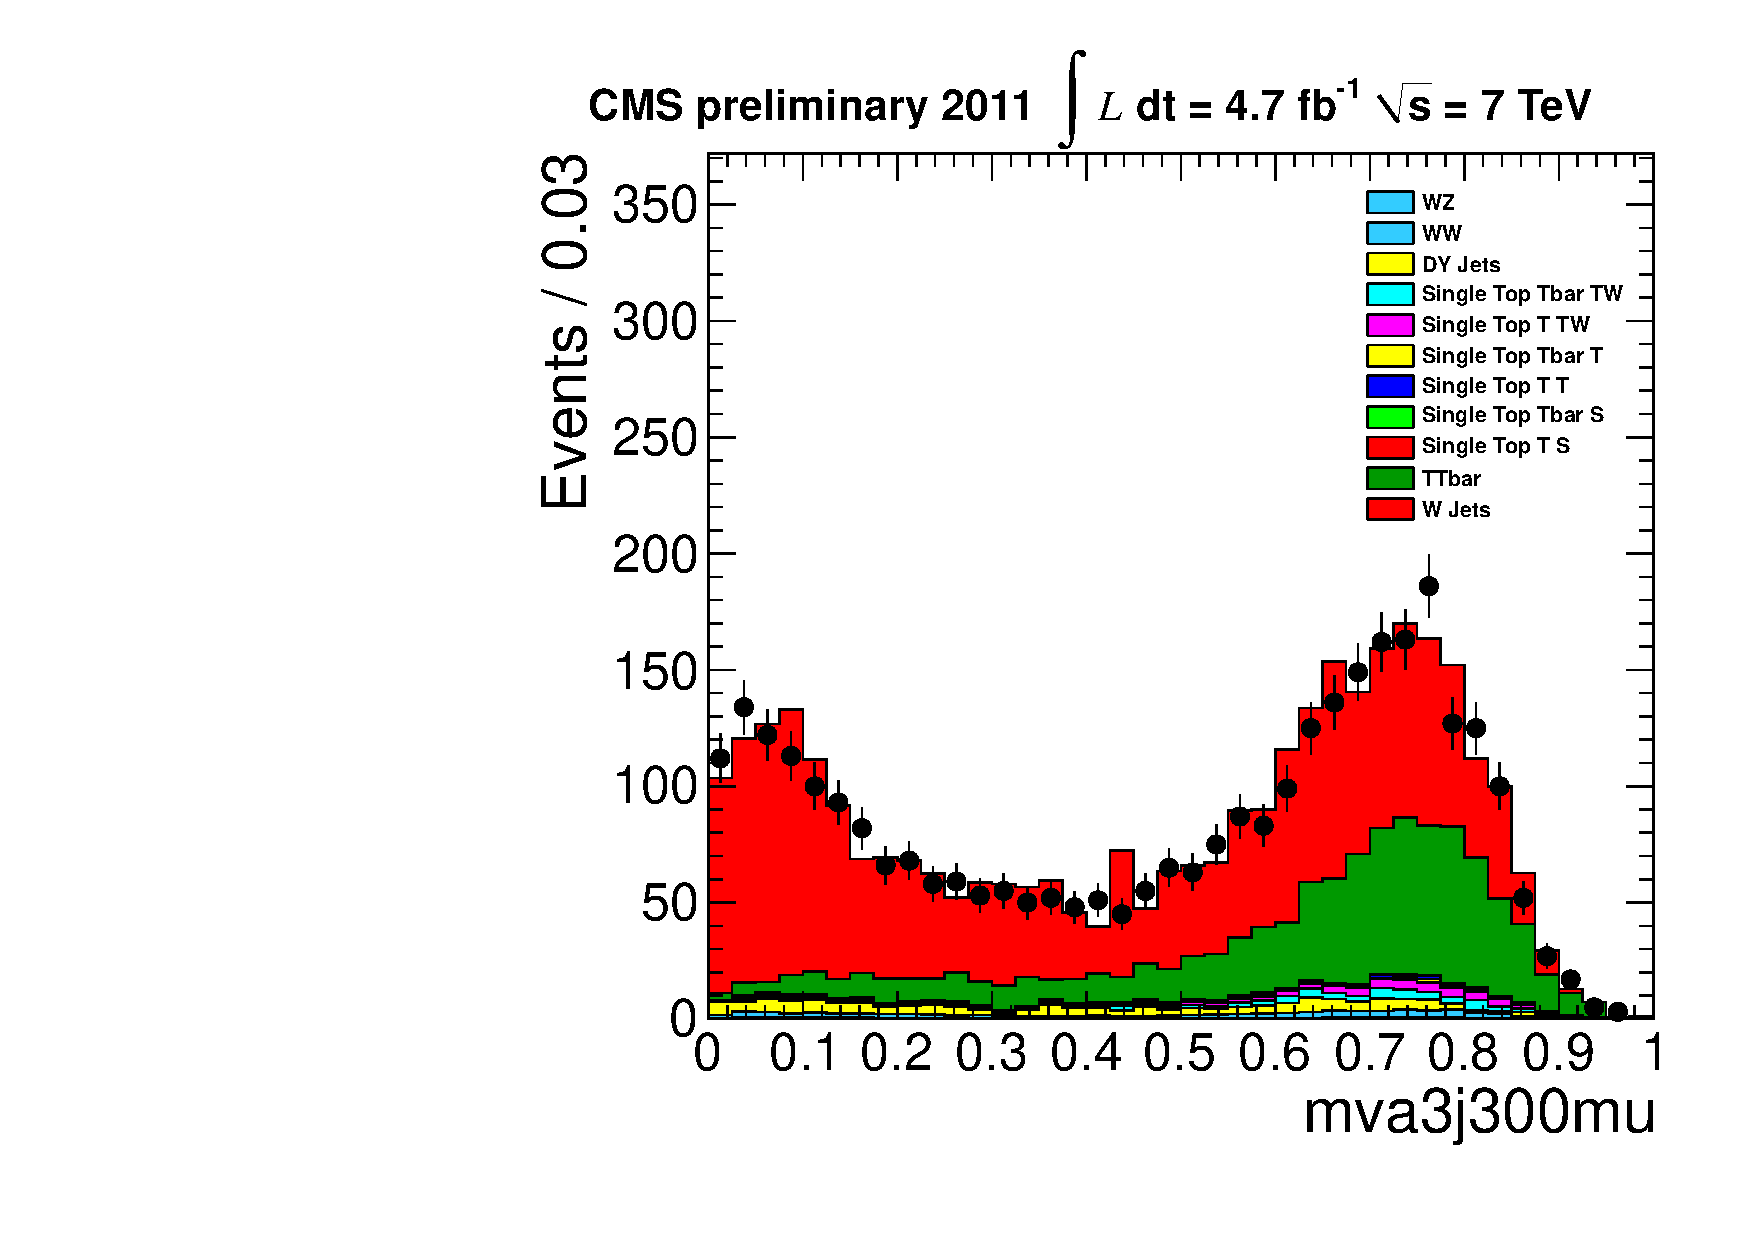
\includegraphics[width=0.49\textwidth]{figs/cl-mva3j300mu-normal.pdf}
  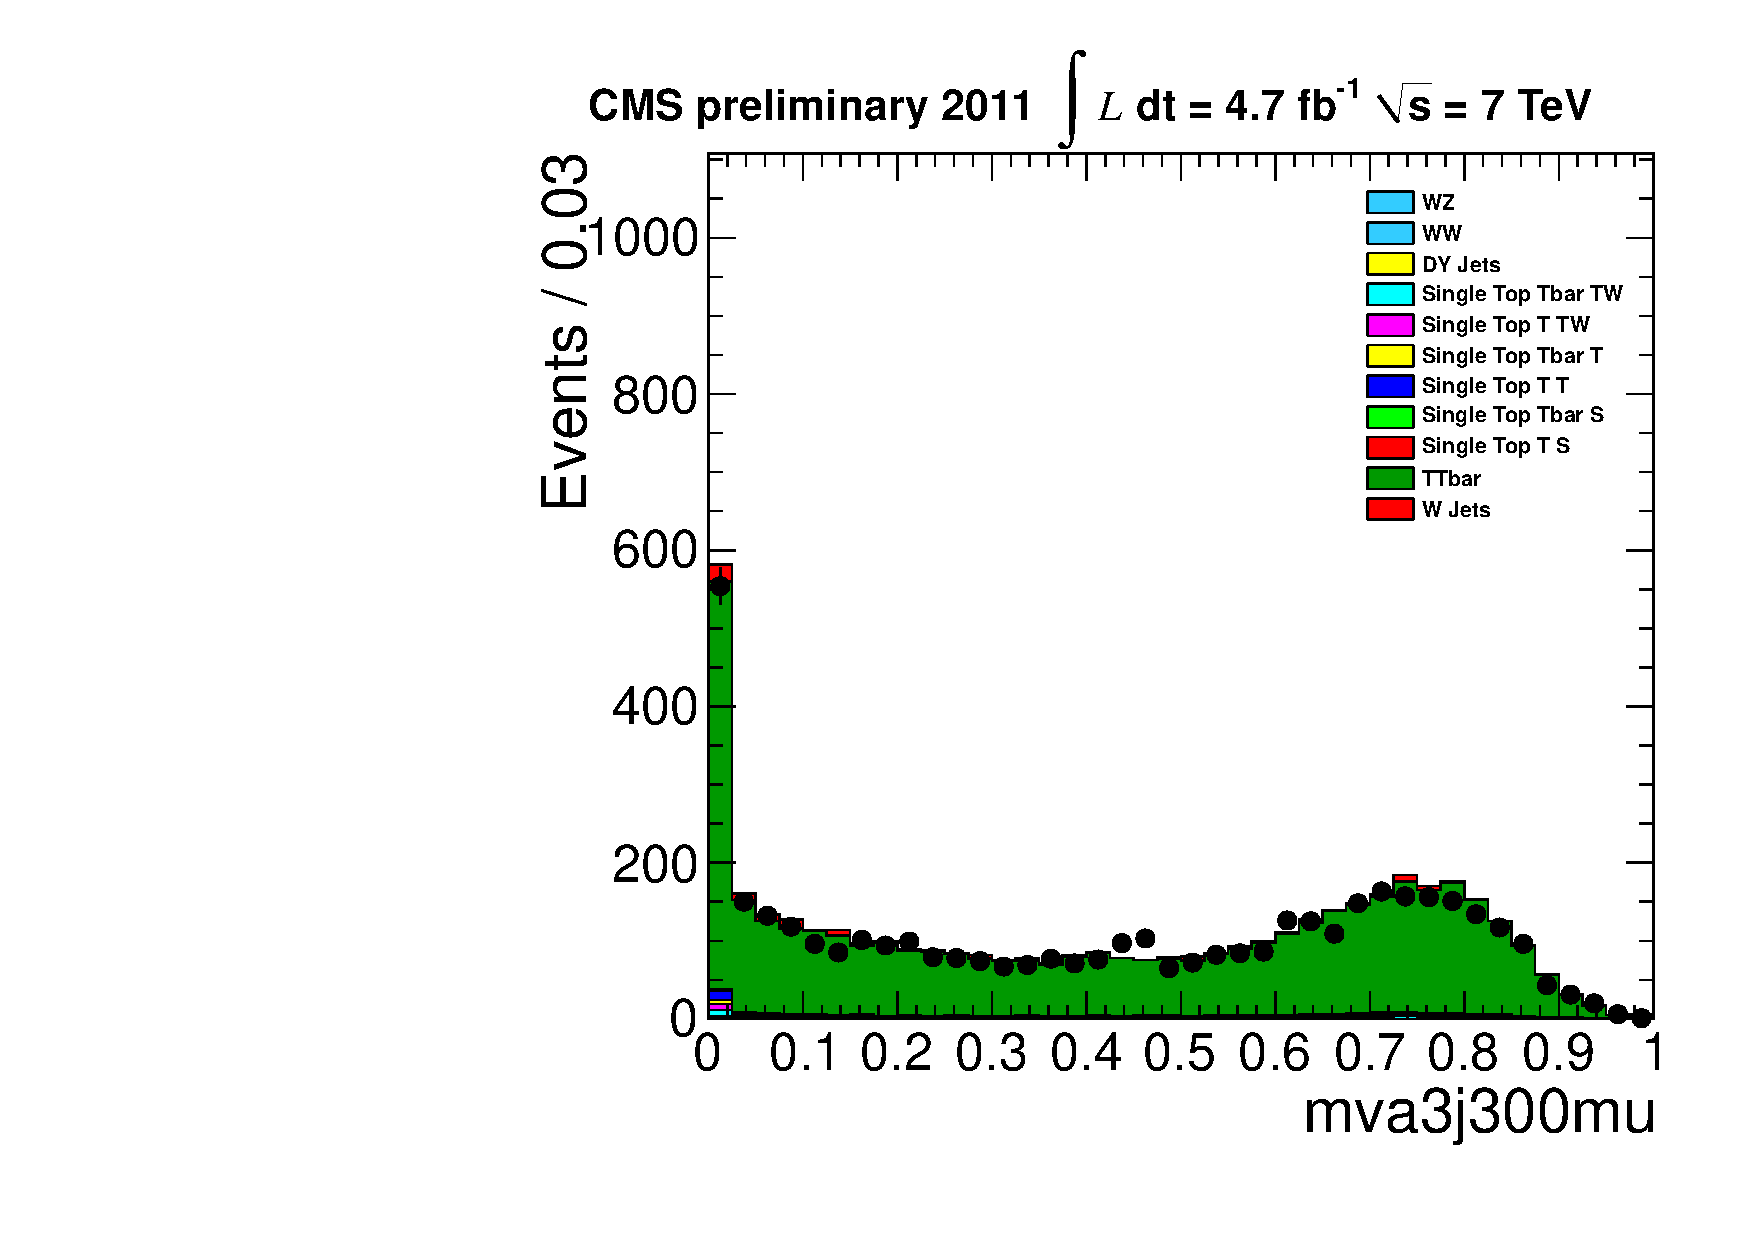
\includegraphics[width=0.49\textwidth]{figs/cl-mva3j300mu-inTTbar.pdf}
  \caption{\label{fig:mva:plots-mva3j300mu} The data-MC comparisons
    after standard event selection (left) and top pair
    selection (right) for the working point: mva3j300mu.}
\end{figure}

%%%%%%%%%%%%%%%%%%% mva3j350mu
\begin{figure}[!t]
  \centering
  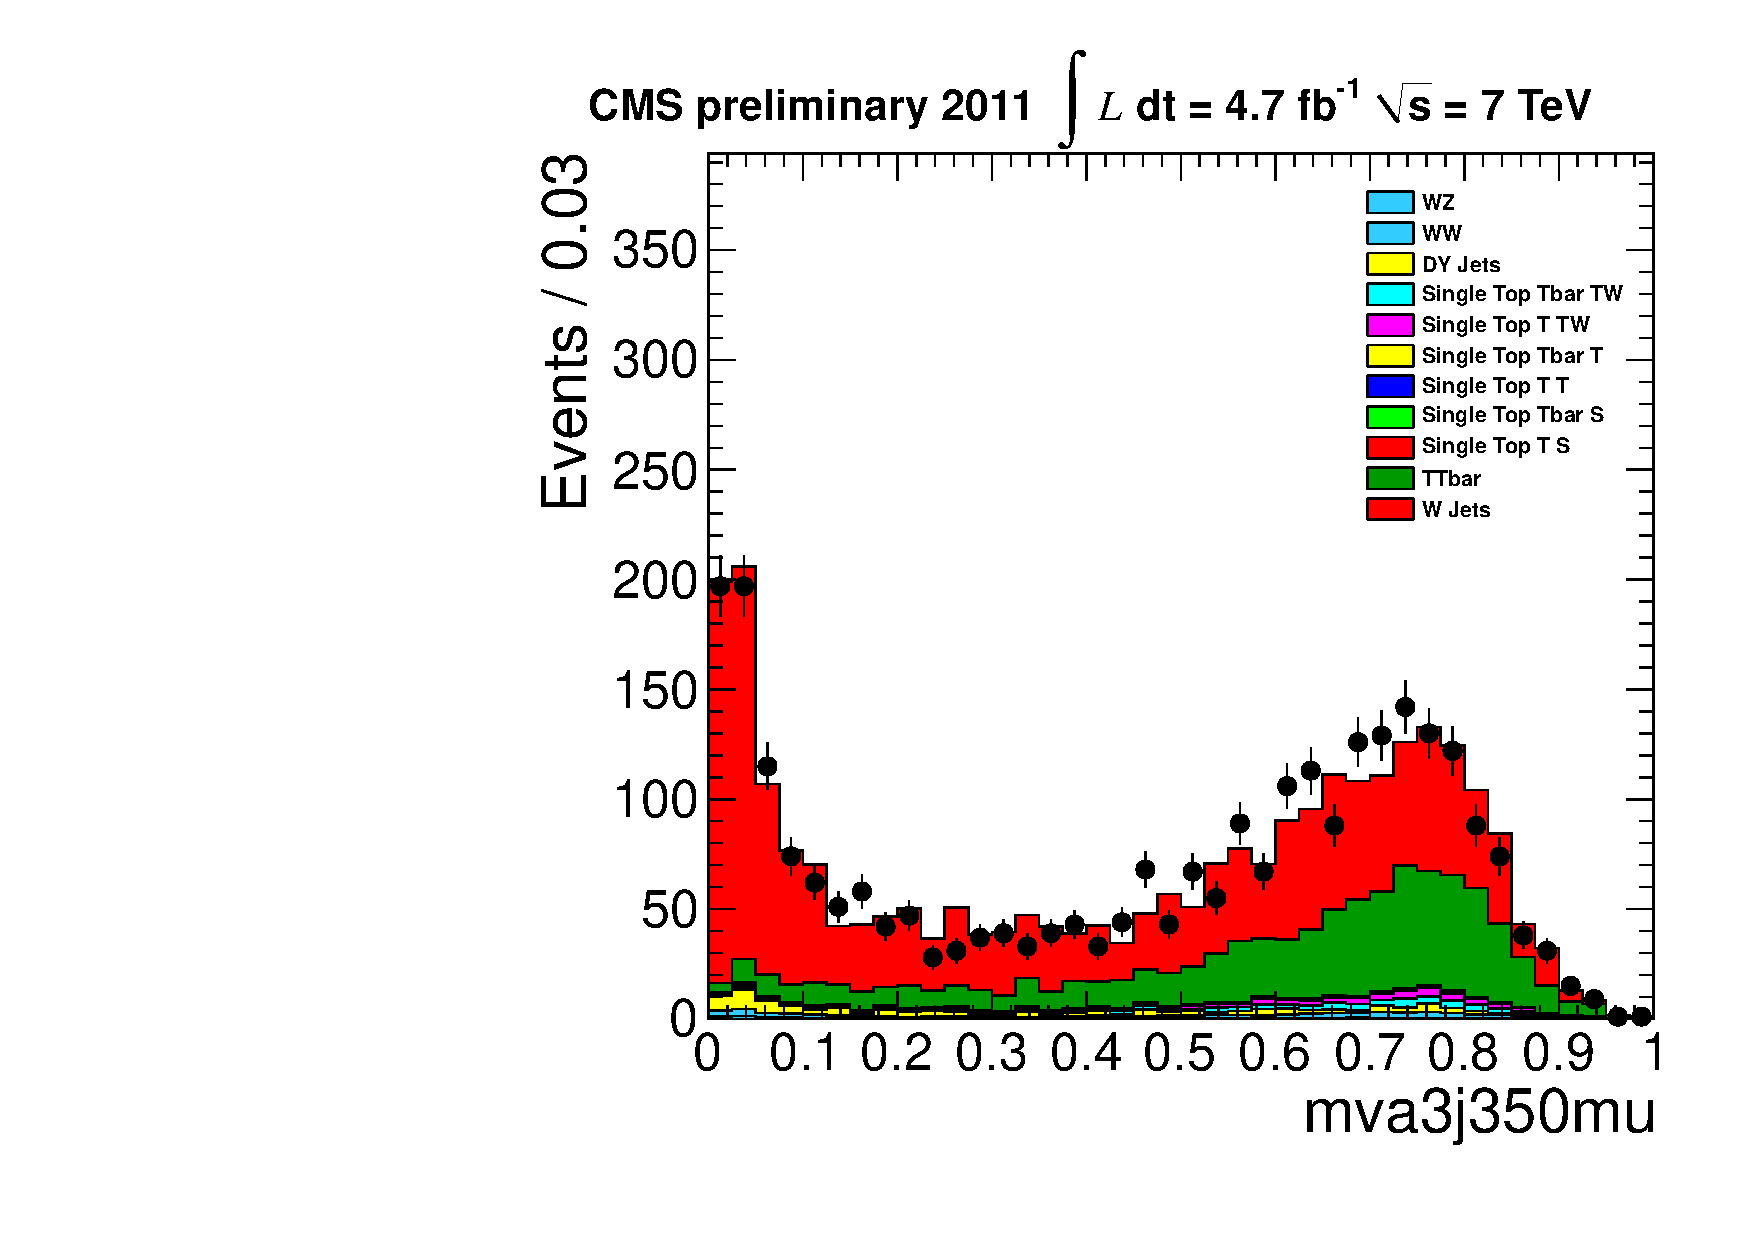
\includegraphics[width=0.49\textwidth]{figs/cl-mva3j350mu-normal.pdf}
  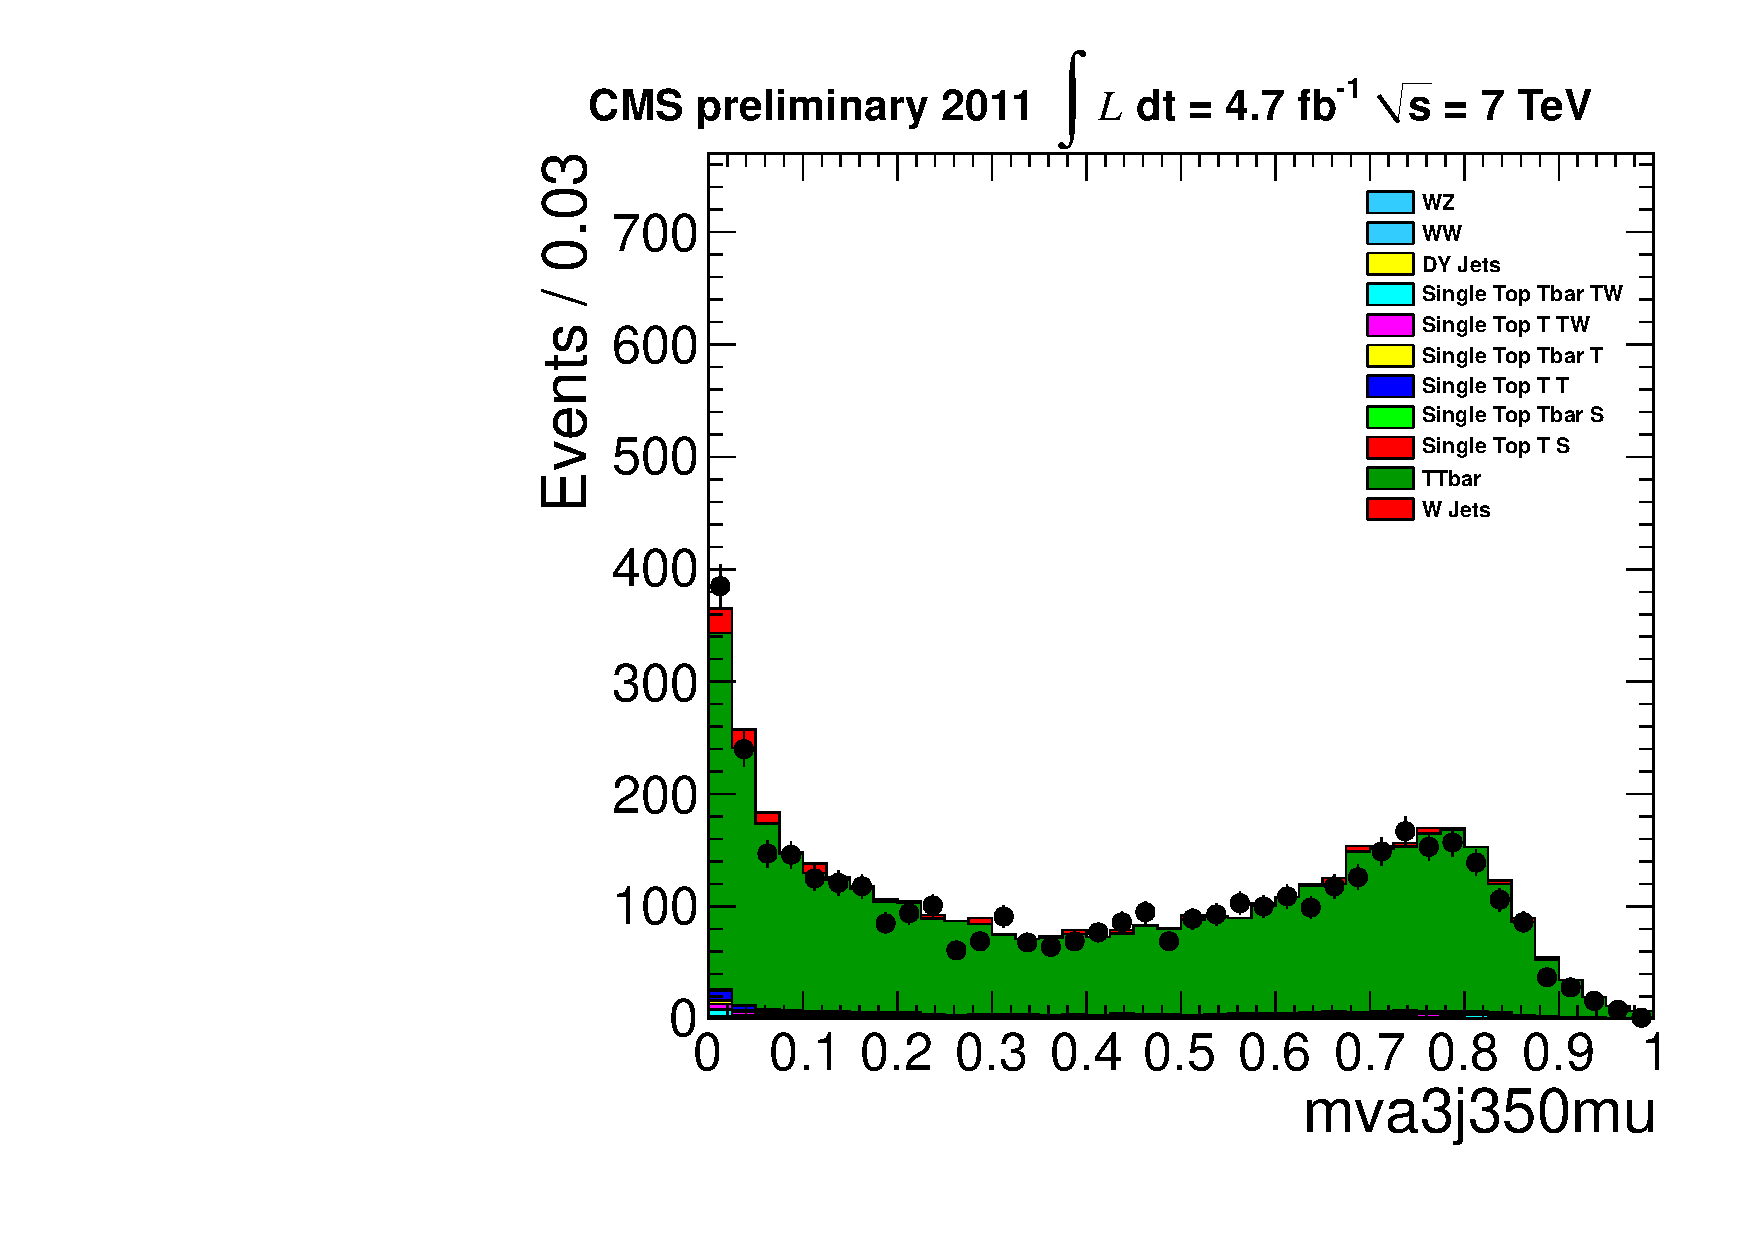
\includegraphics[width=0.49\textwidth]{figs/cl-mva3j350mu-inTTbar.pdf}
  \caption{\label{fig:mva:plots-mva3j350mu} The data-MC comparisons
    after standard event selection (left) and top pair
    selection (right) for the working point: mva3j350mu.}
\end{figure}

%%%%%%%%%%%%%%%%%%% mva3j400mu
\begin{figure}[!t]
  \centering
  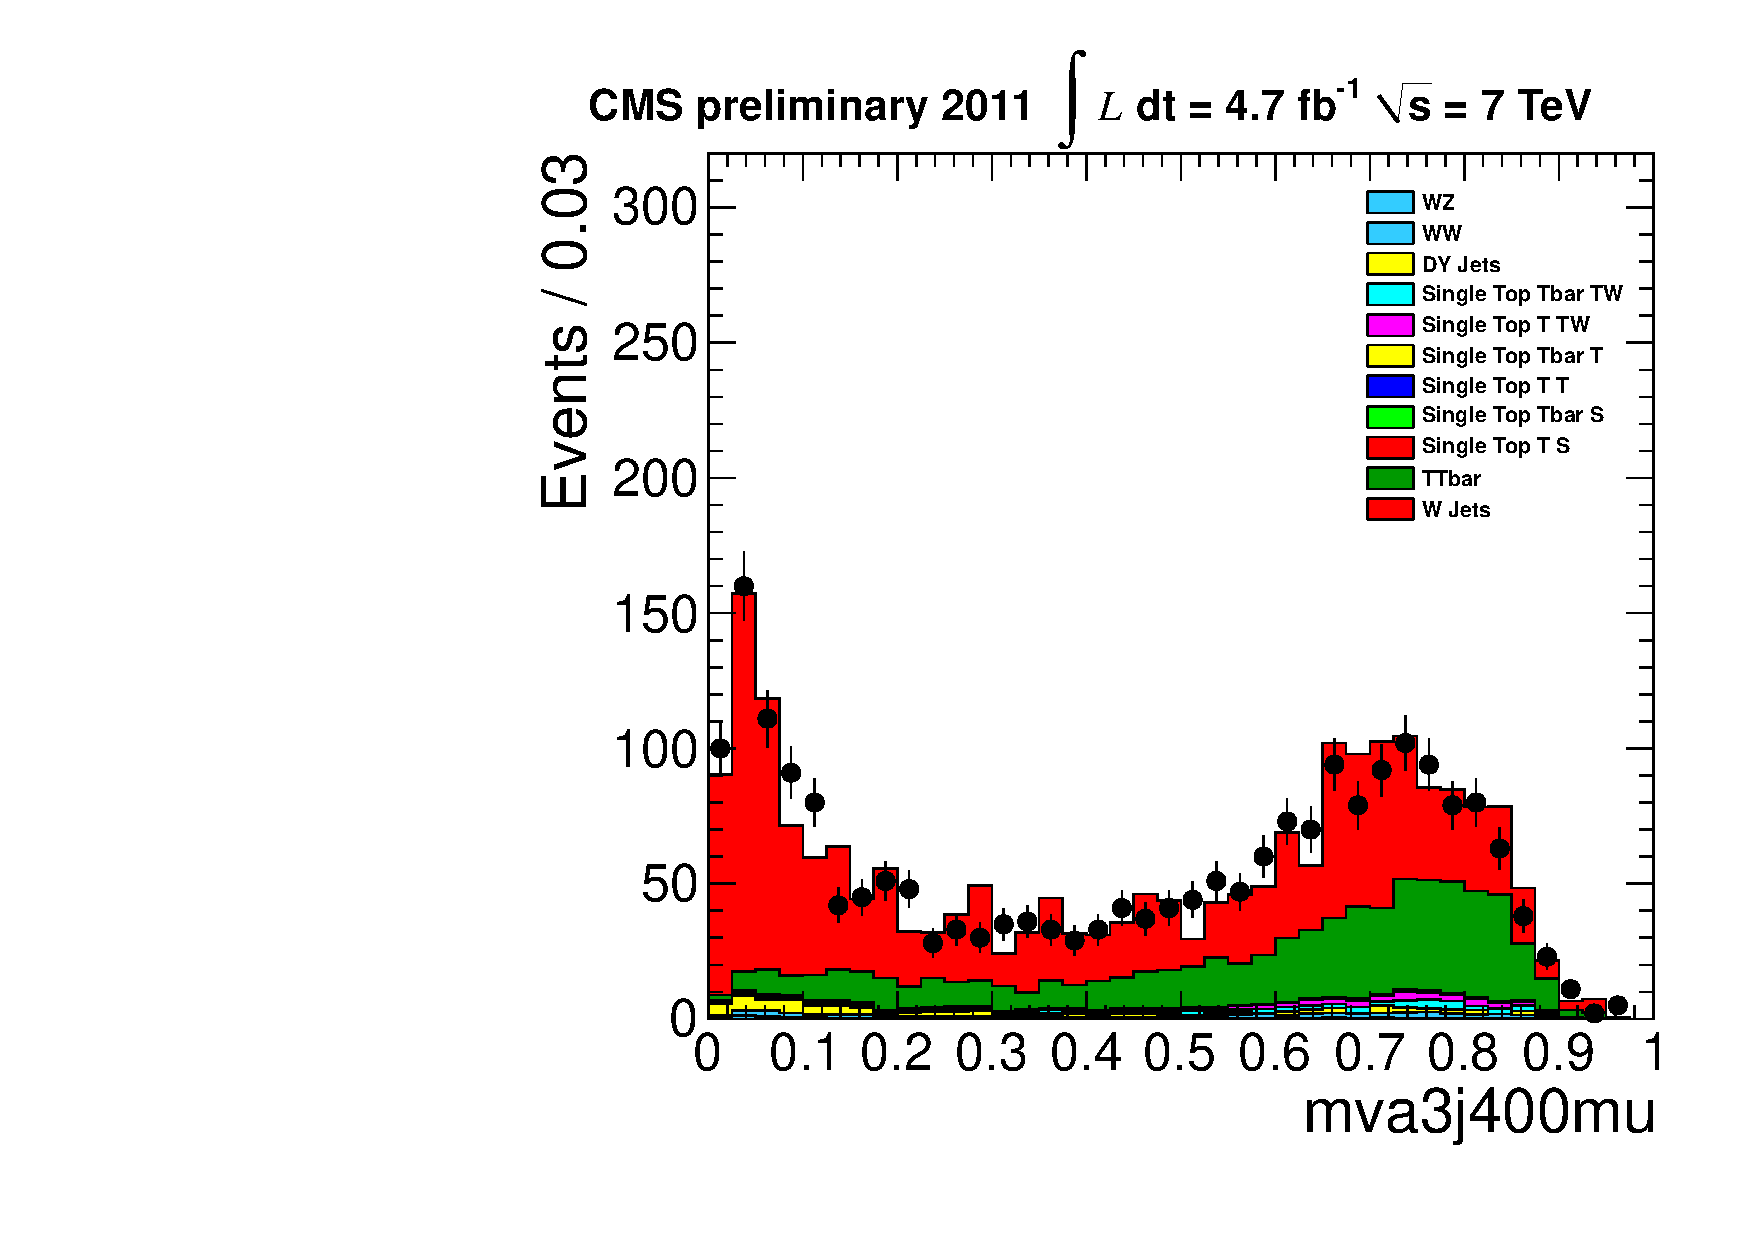
\includegraphics[width=0.49\textwidth]{figs/cl-mva3j400mu-normal.pdf}
  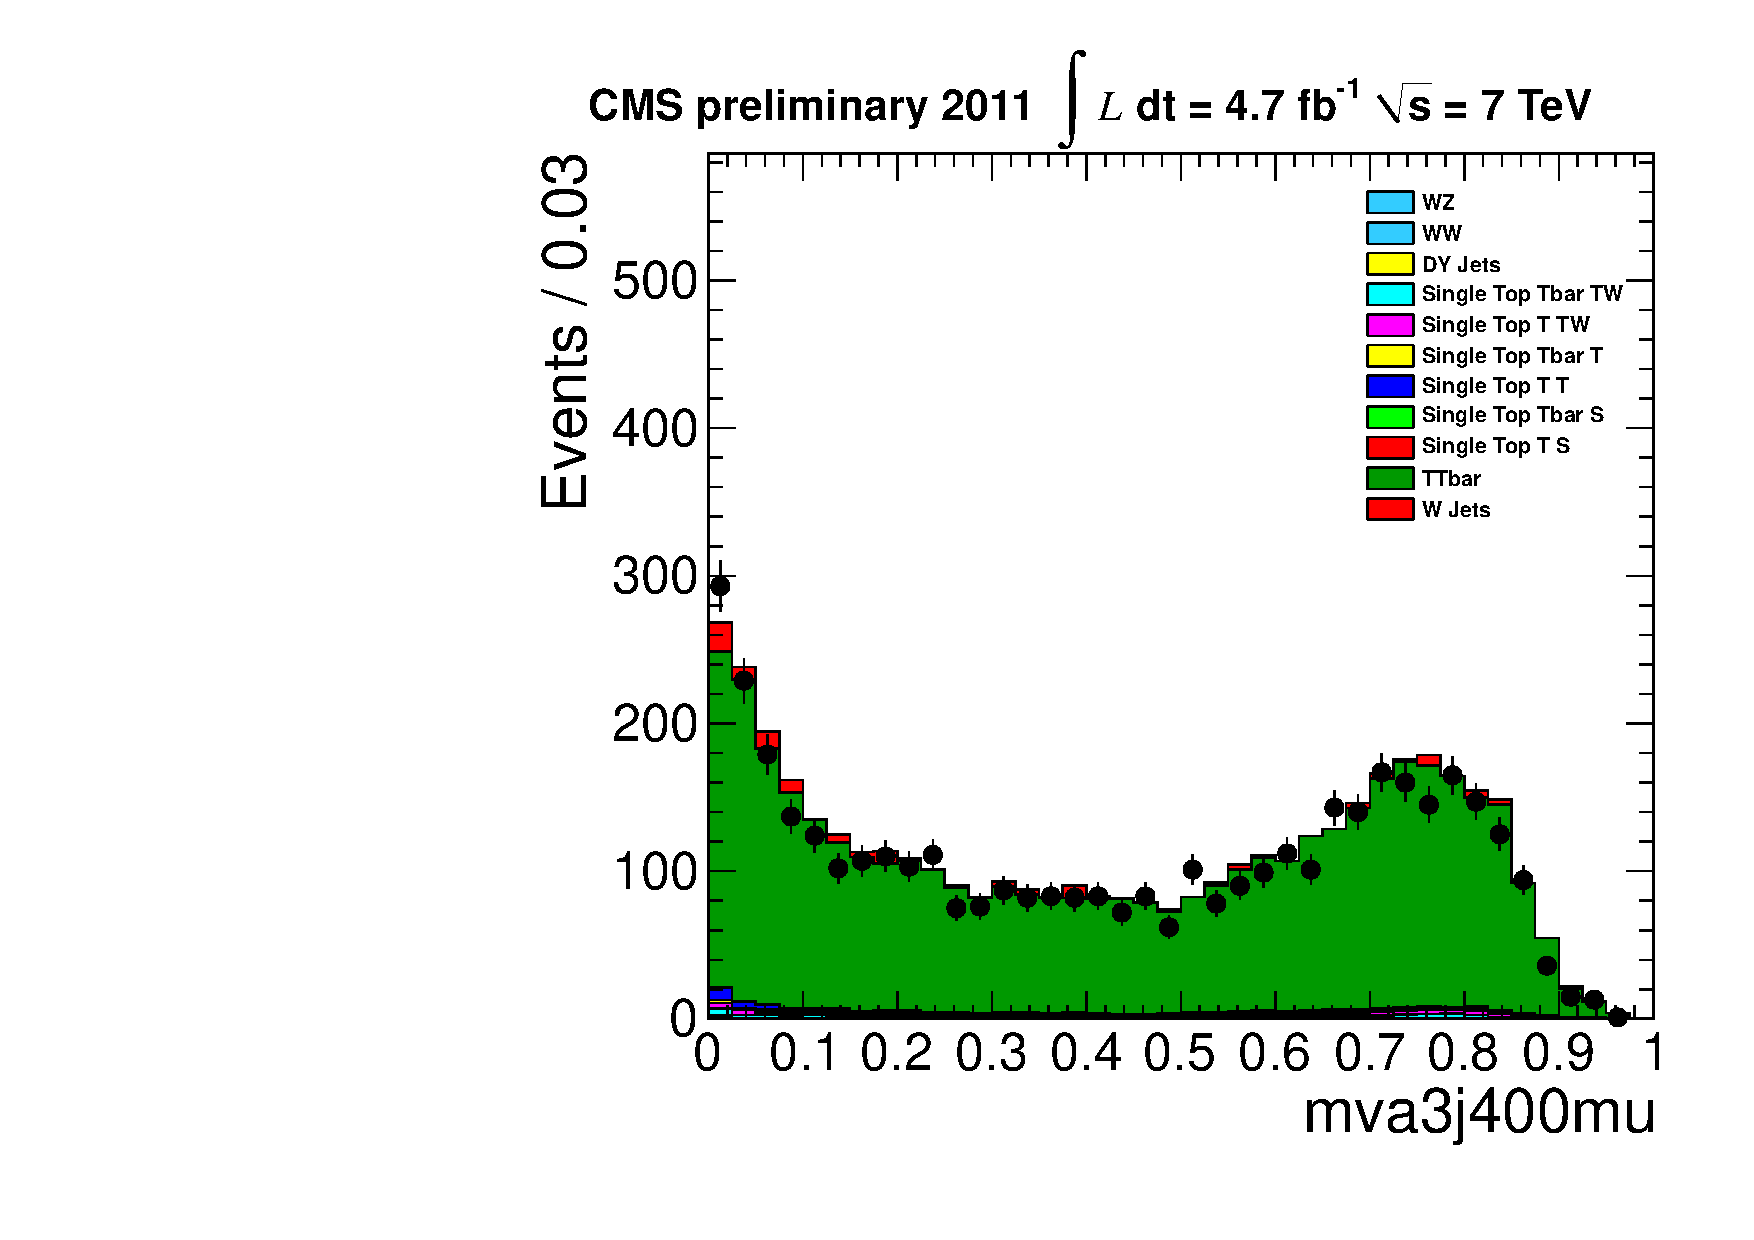
\includegraphics[width=0.49\textwidth]{figs/cl-mva3j400mu-inTTbar.pdf}
  \caption{\label{fig:mva:plots-mva3j400mu} The data-MC comparisons
    after standard event selection (left) and top pair
    selection (right) for the working point: mva3j400mu.}
\end{figure}

%%%%%%%%%%%%%%%%%%% mva3j450mu
\begin{figure}[!t]
  \centering
  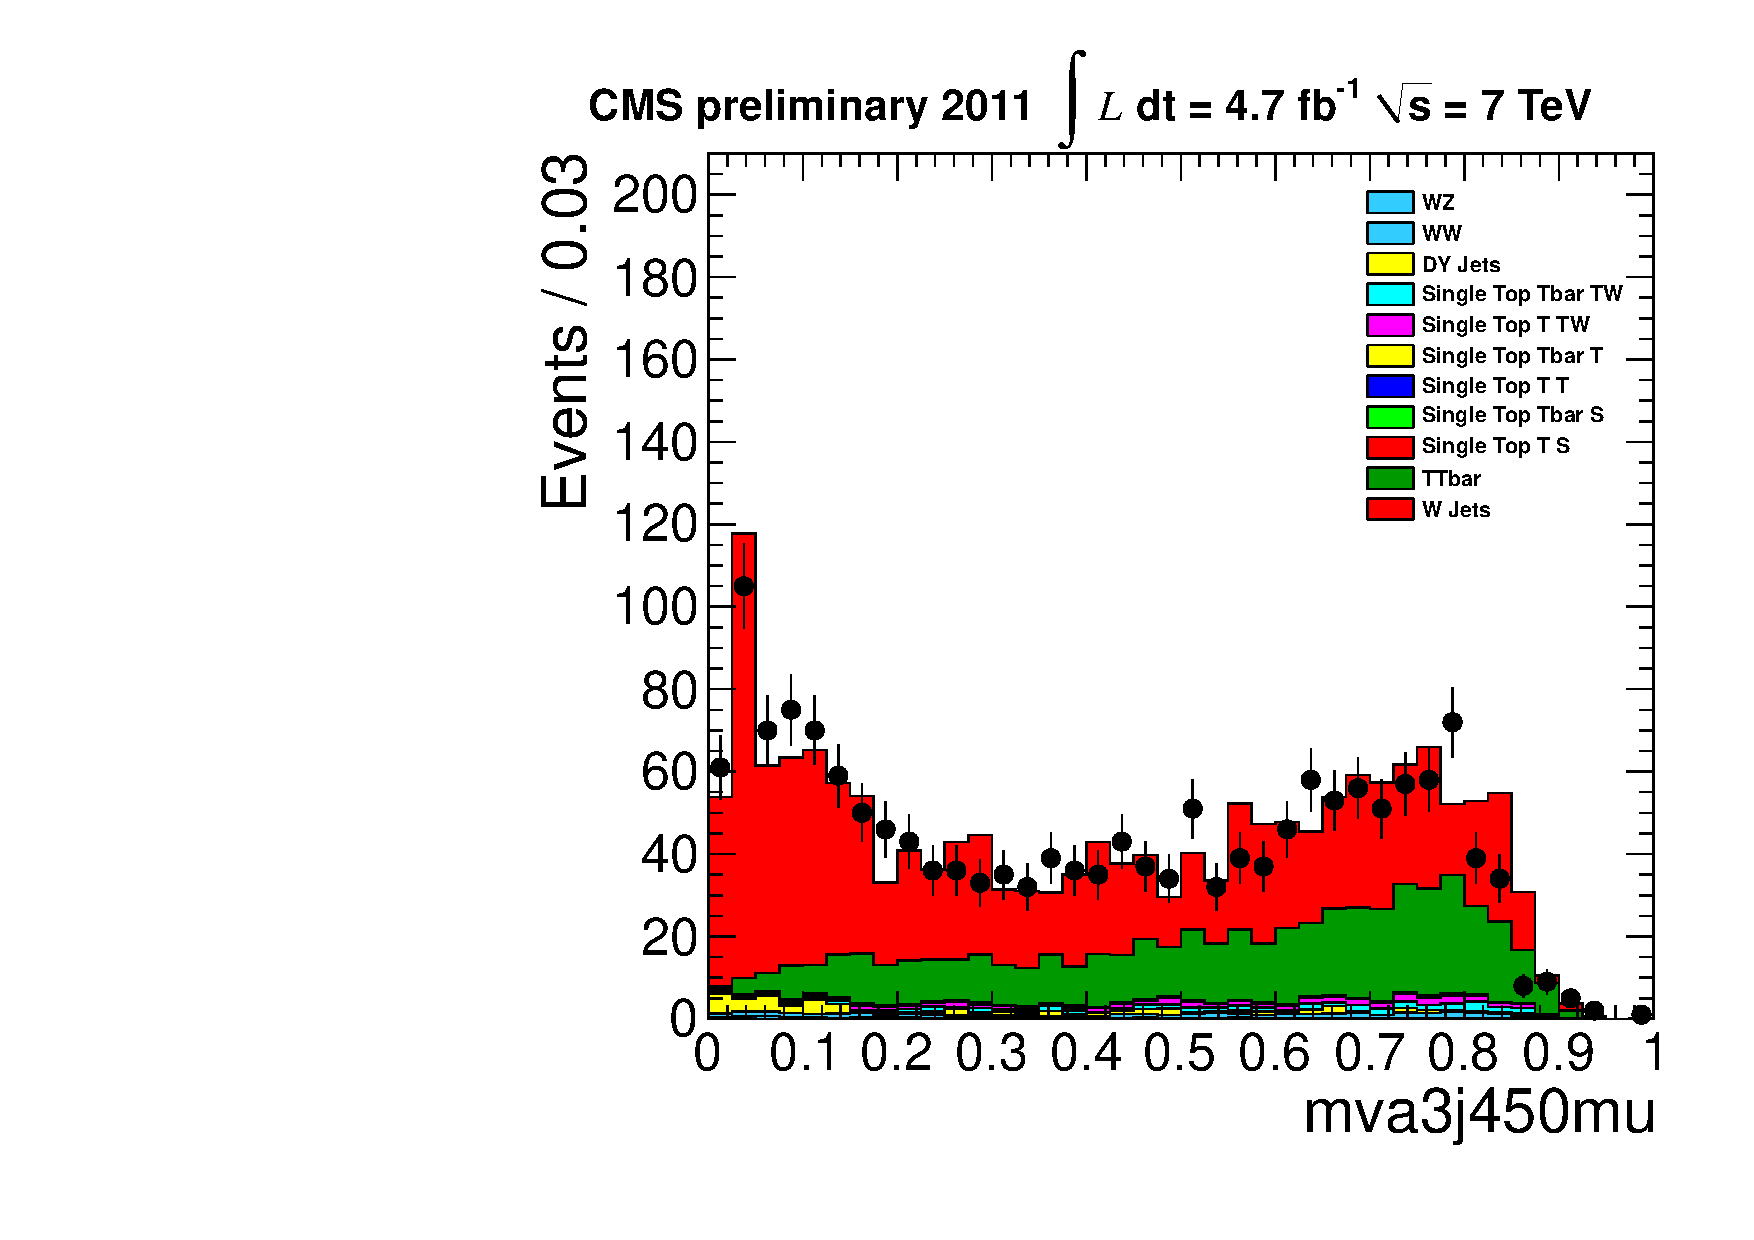
\includegraphics[width=0.49\textwidth]{figs/cl-mva3j450mu-normal.pdf}
  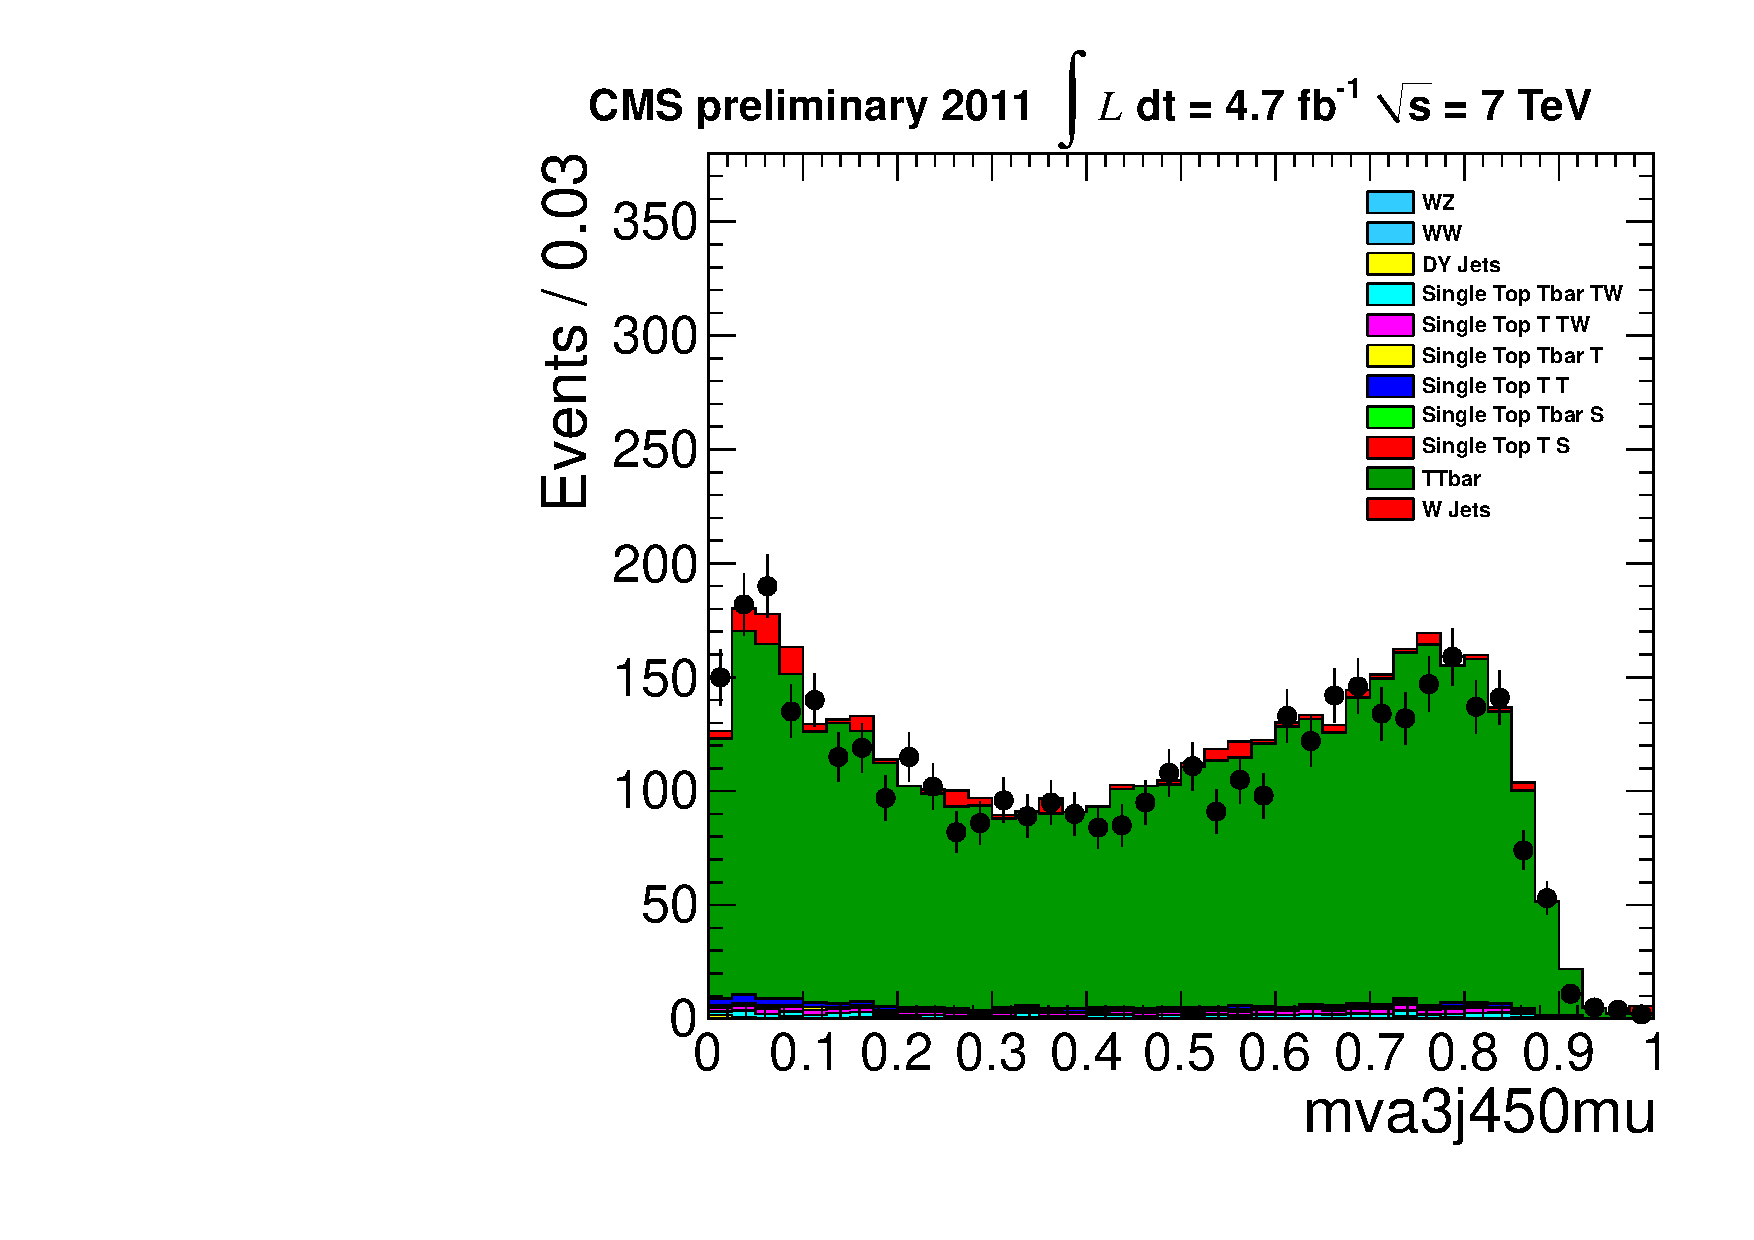
\includegraphics[width=0.49\textwidth]{figs/cl-mva3j450mu-inTTbar.pdf}
  \caption{\label{fig:mva:plots-mva3j450mu} The data-MC comparisons
    after standard event selection (left) and top pair
    selection (right) for the working point: mva3j450mu.}
\end{figure}

%%%%%%%%%%%%%%%%%%% mva3j500mu
\begin{figure}[!t]
  \centering
  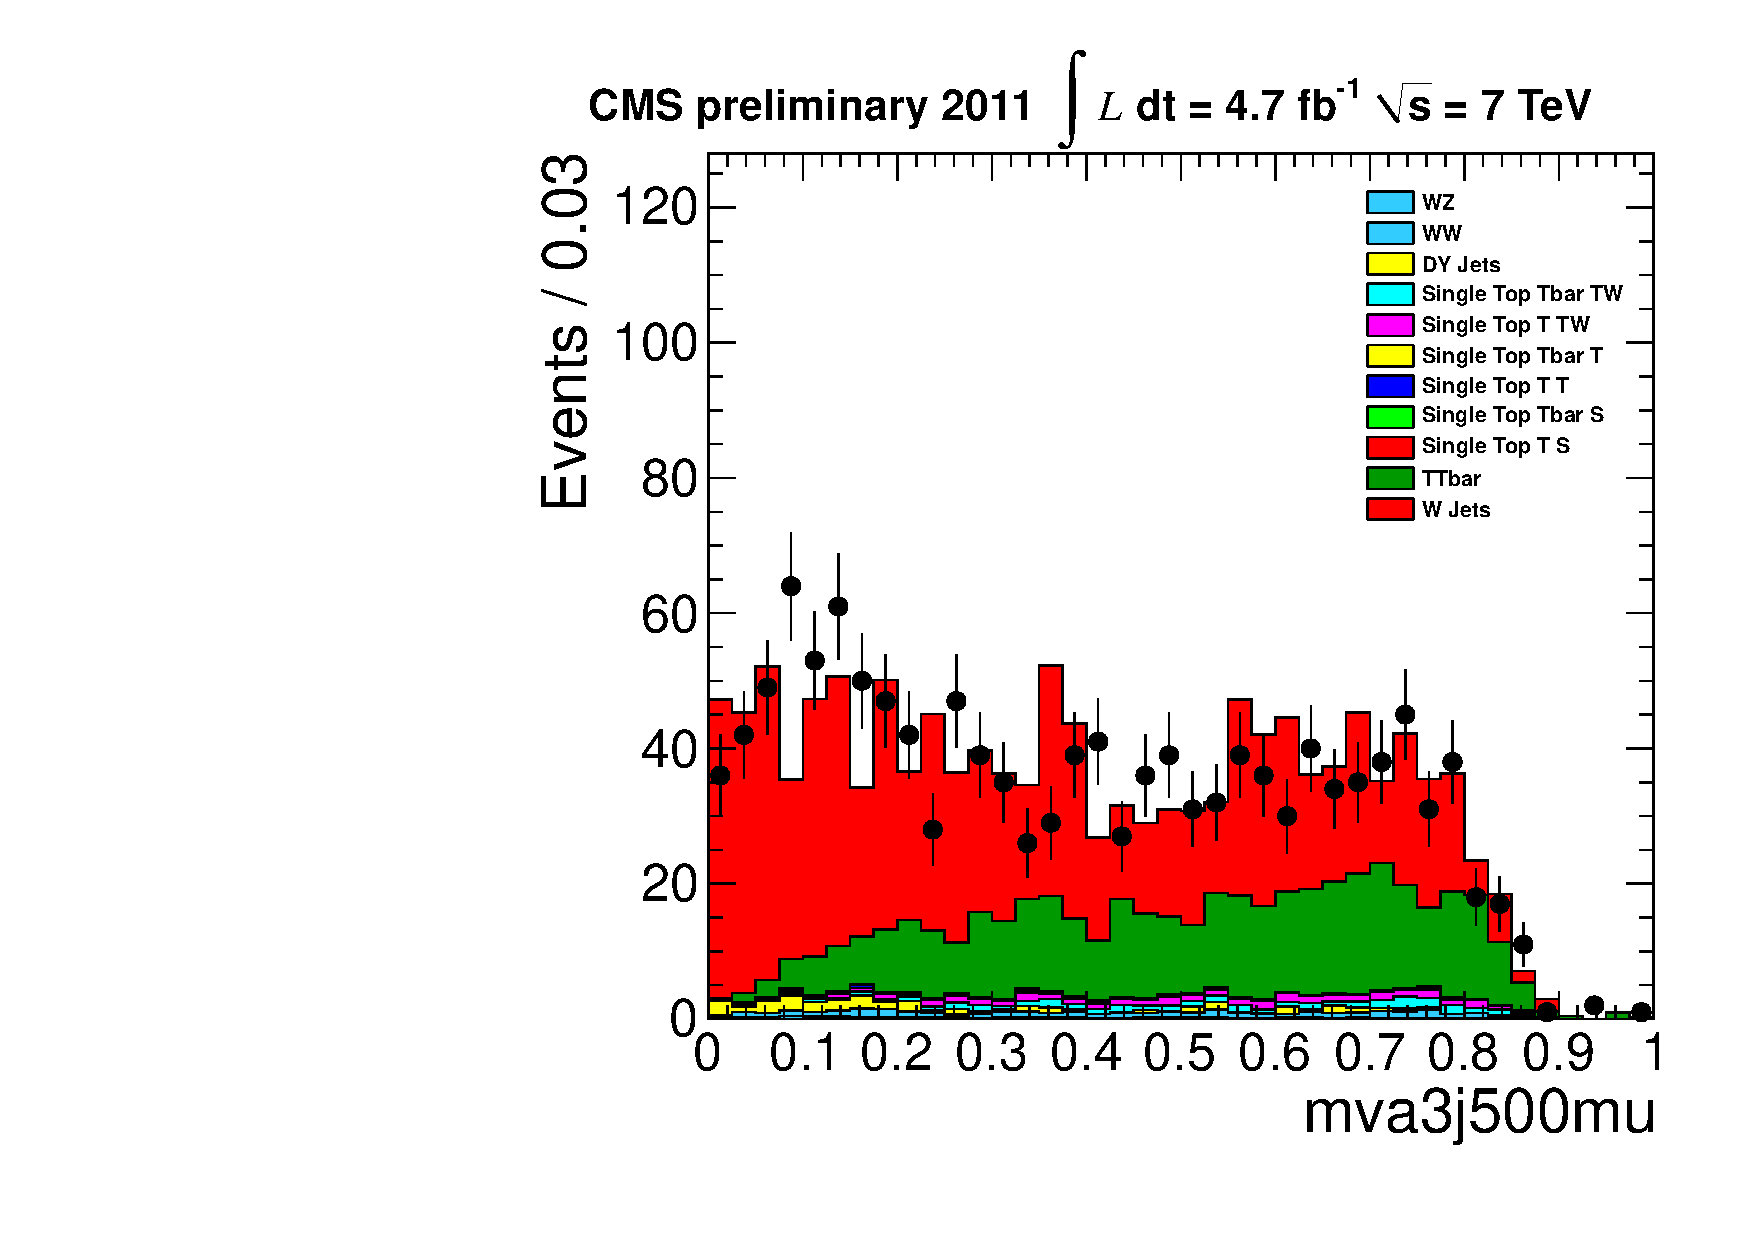
\includegraphics[width=0.49\textwidth]{figs/cl-mva3j500mu-normal.pdf}
  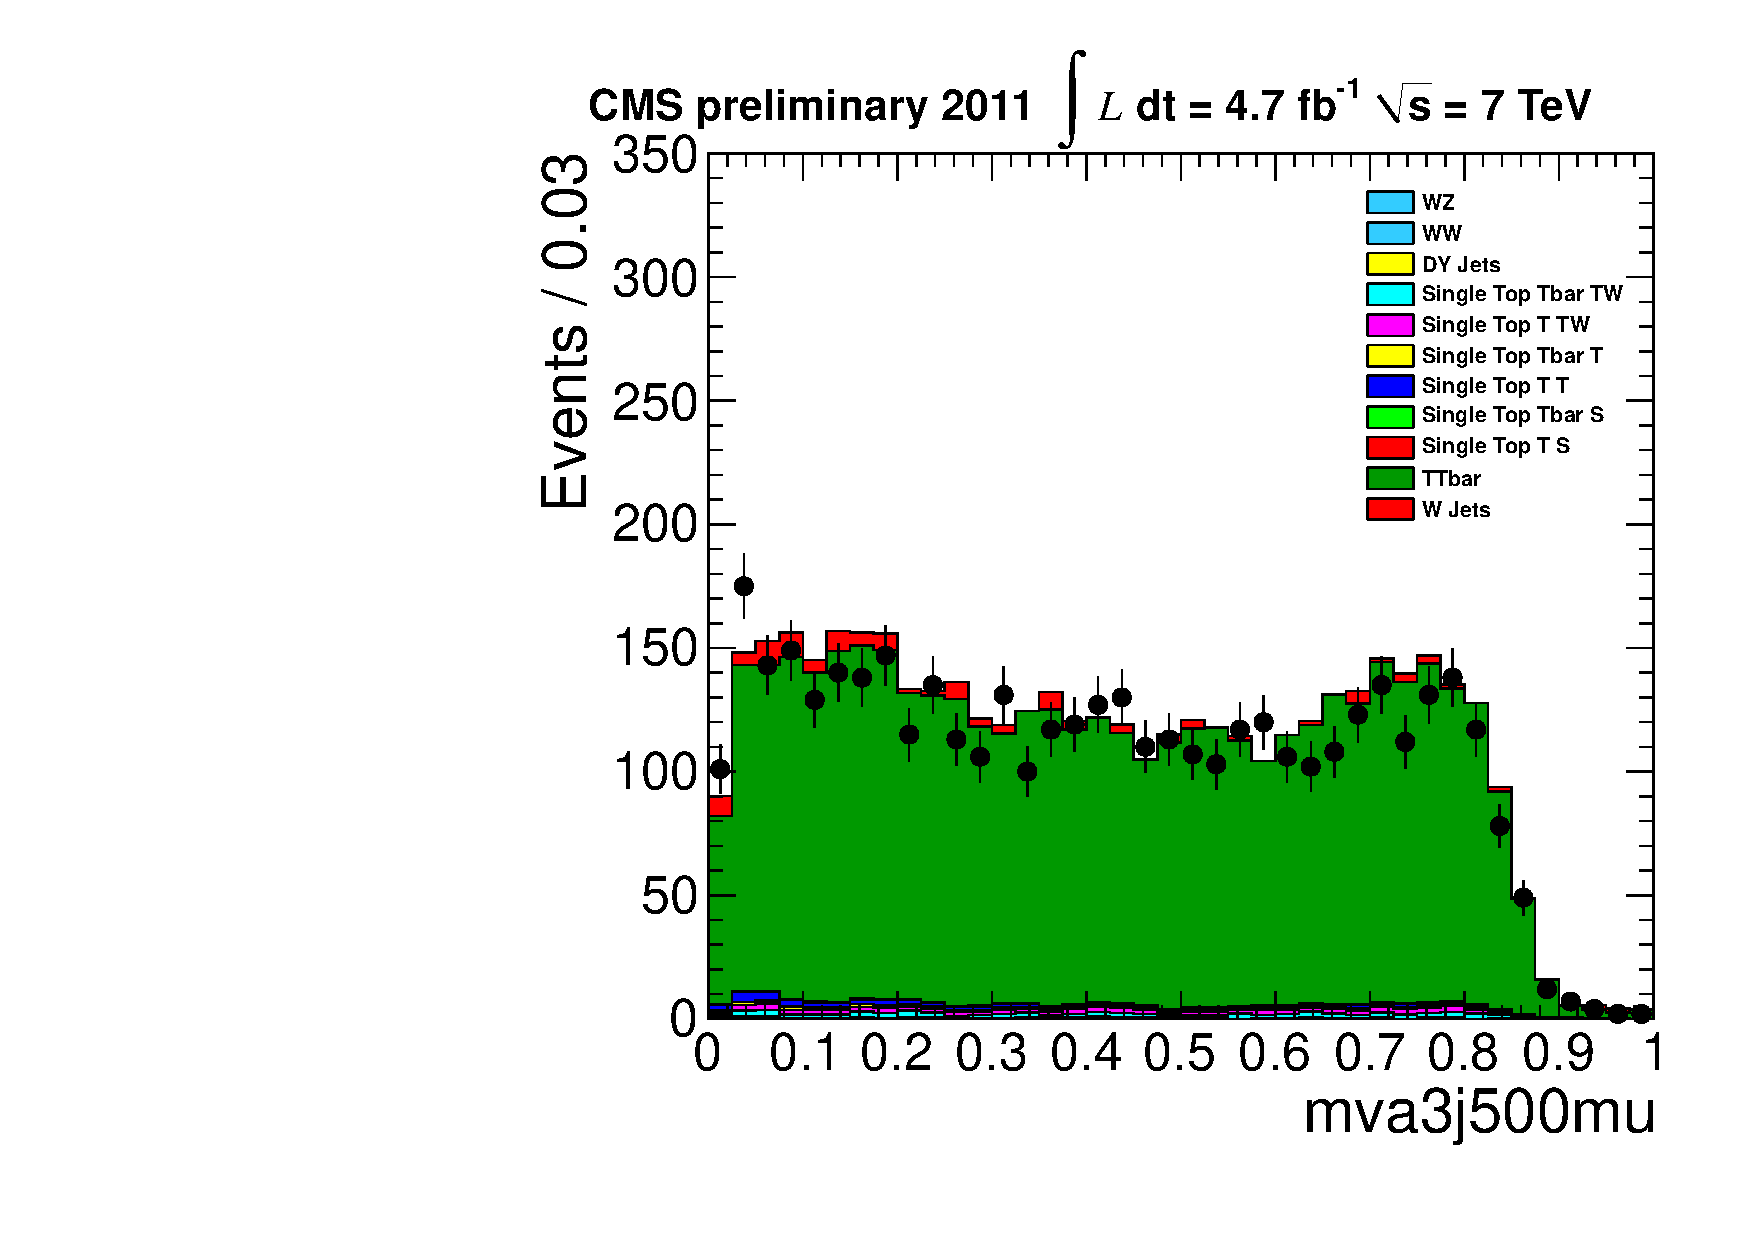
\includegraphics[width=0.49\textwidth]{figs/cl-mva3j500mu-inTTbar.pdf}
  \caption{\label{fig:mva:plots-mva3j500mu} The data-MC comparisons
    after standard event selection (left) and top pair
    selection (right) for the working point: mva3j500mu.}
\end{figure}

%%%%%%%%%%%%%%%%%%% mva3j550mu
\begin{figure}[!t]
  \centering
  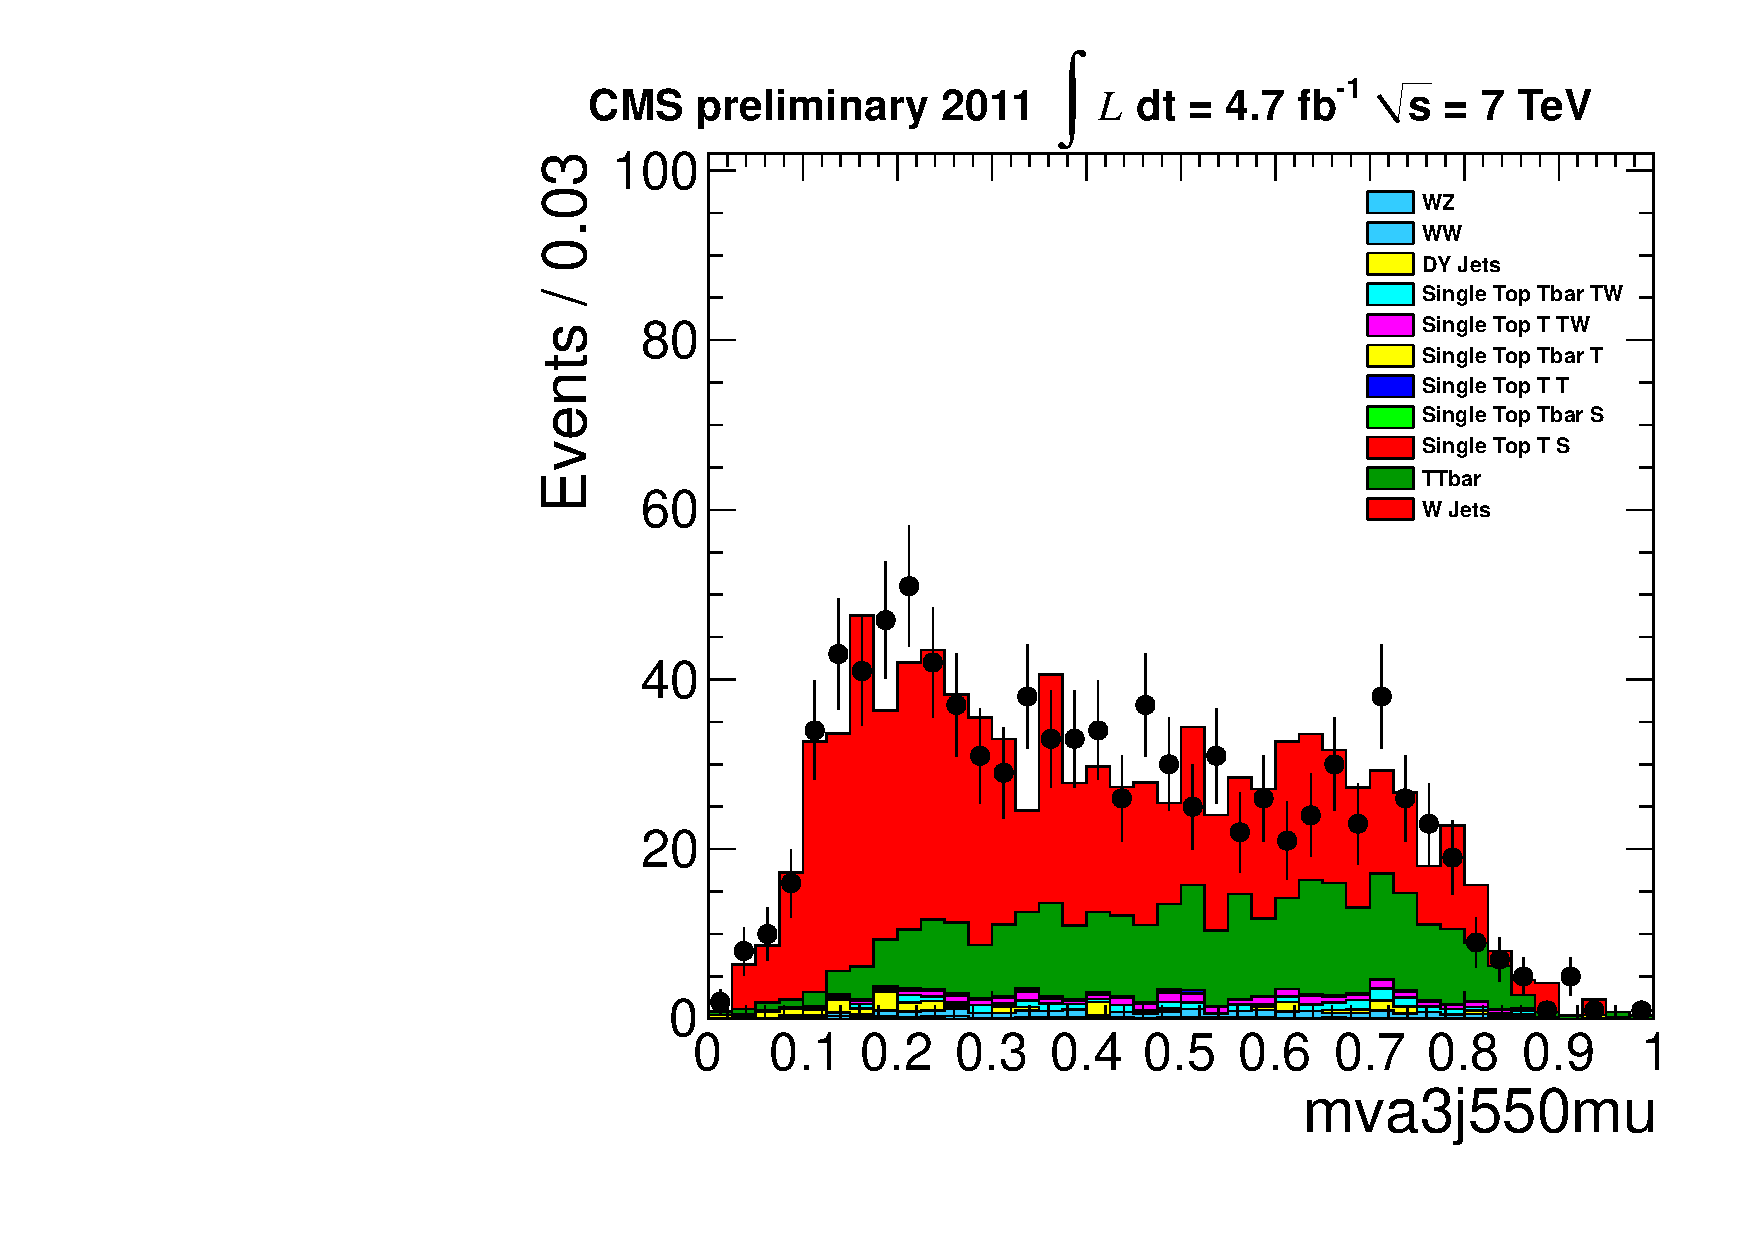
\includegraphics[width=0.49\textwidth]{figs/cl-mva3j550mu-normal.pdf}
  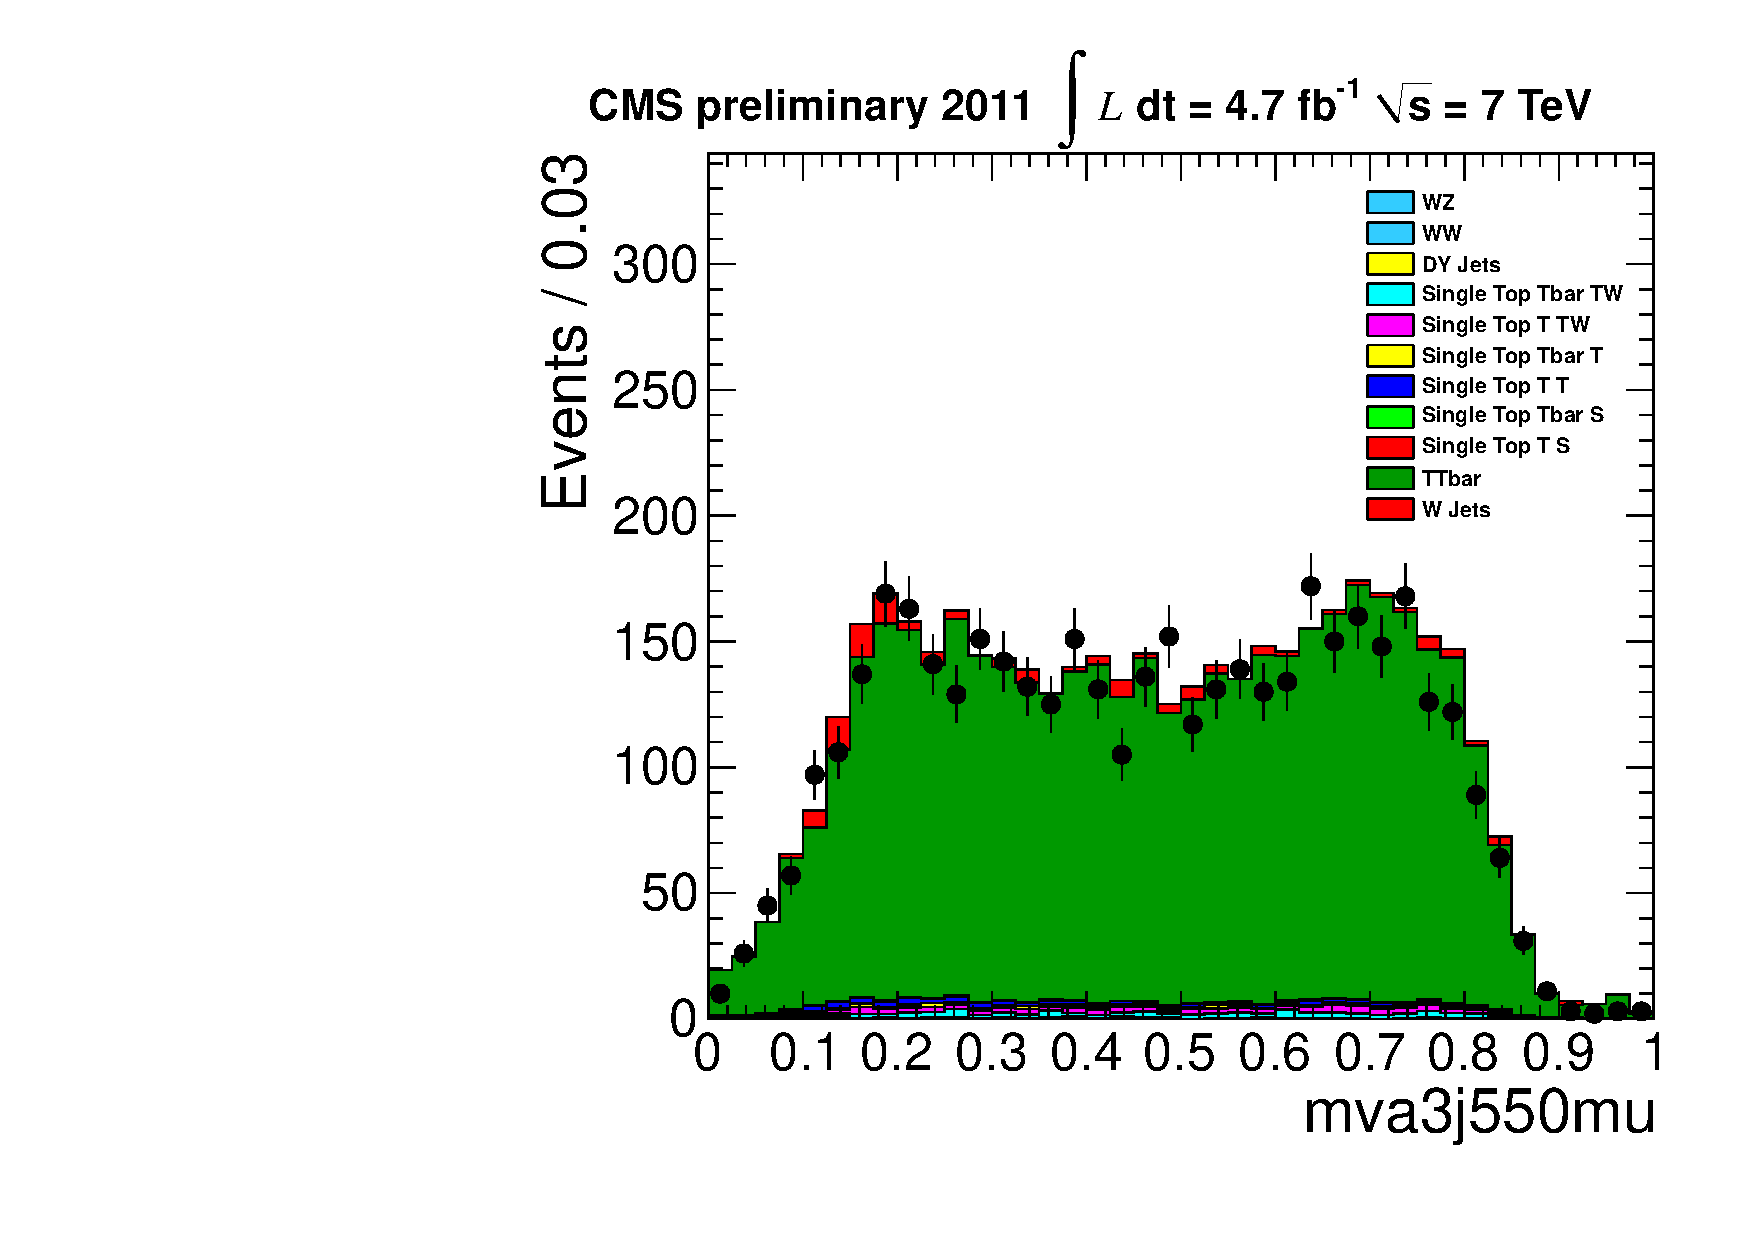
\includegraphics[width=0.49\textwidth]{figs/cl-mva3j550mu-inTTbar.pdf}
  \caption{\label{fig:mva:plots-mva3j550mu} The data-MC comparisons
    after standard event selection (left) and top pair
    selection (right) for the working point: mva3j550mu.}
\end{figure}

%%%%%%%%%%%%%%%%%%% mva3j600mu
\begin{figure}[!t]
  \centering
  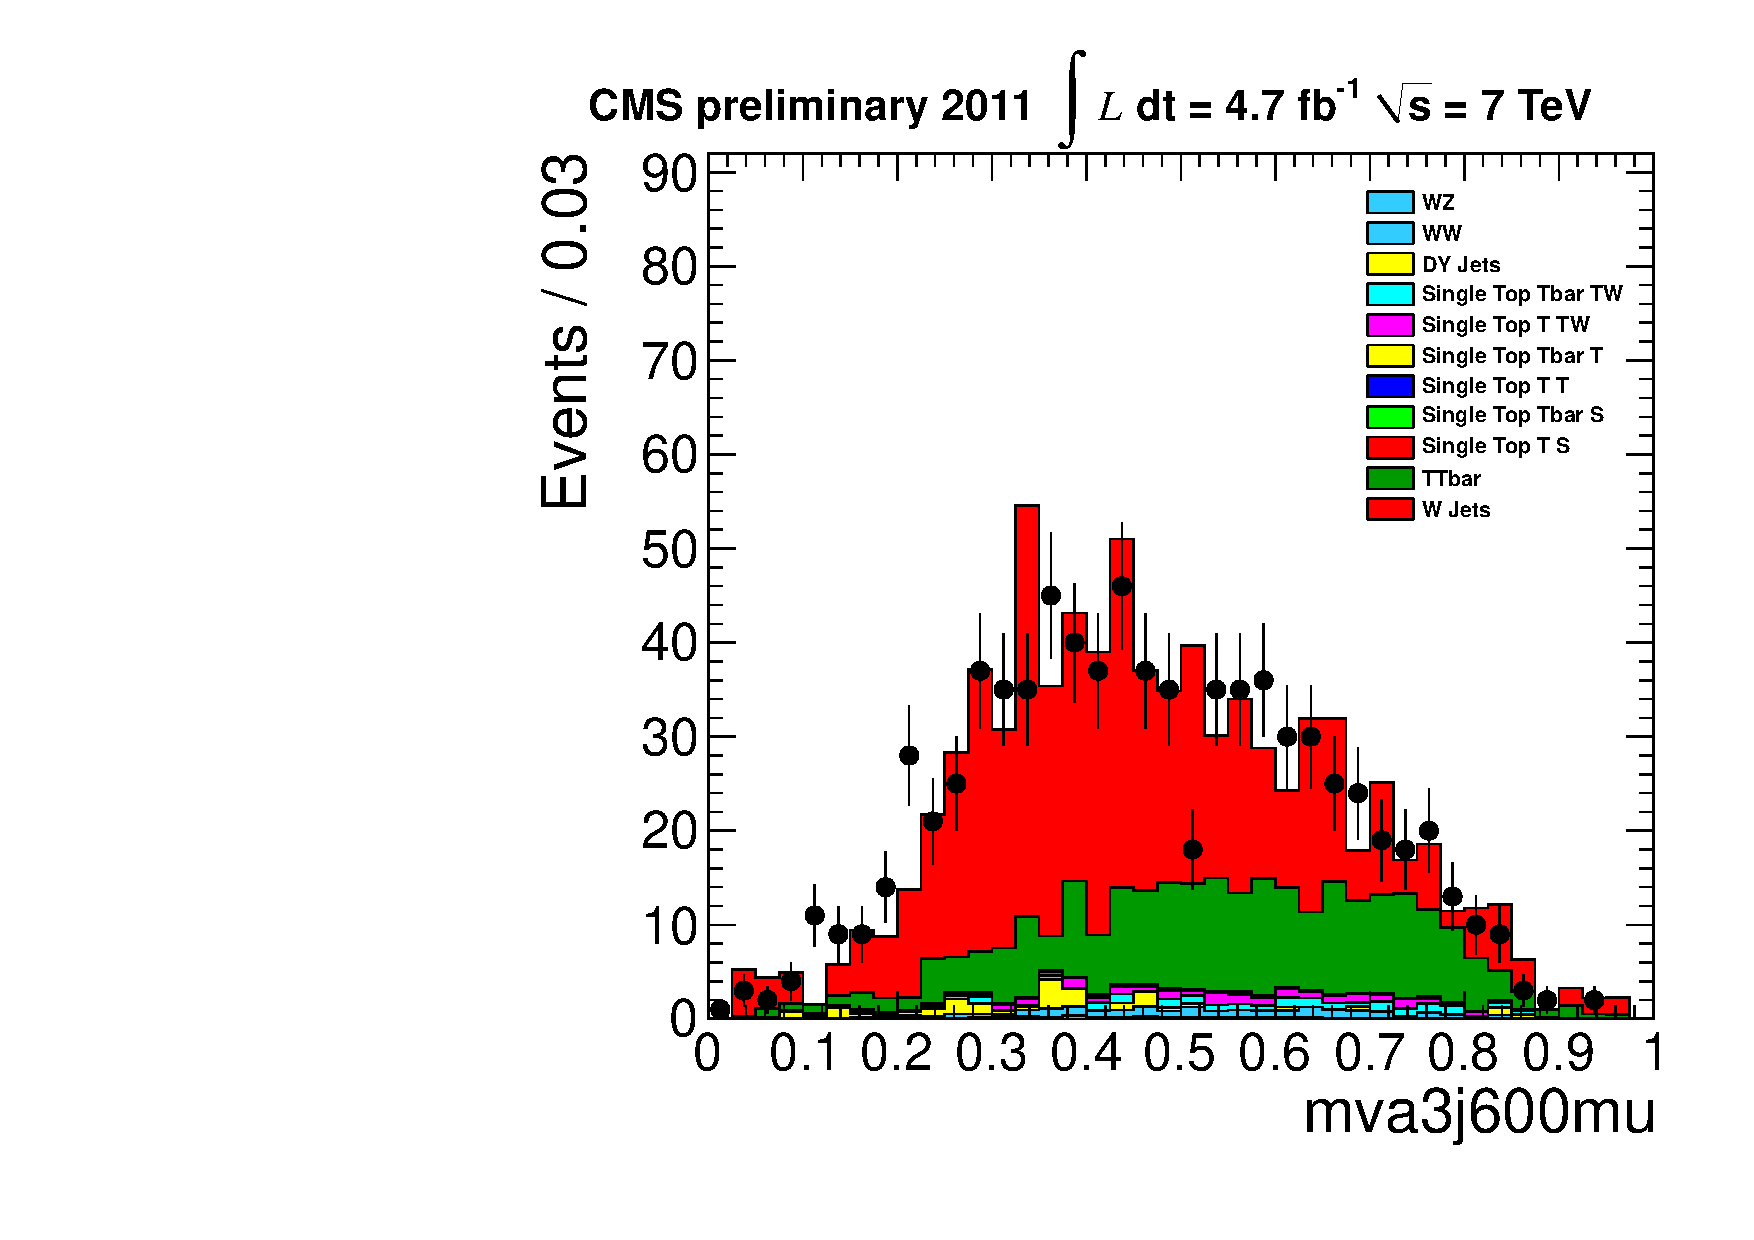
\includegraphics[width=0.49\textwidth]{figs/cl-mva3j600mu-normal.pdf}
  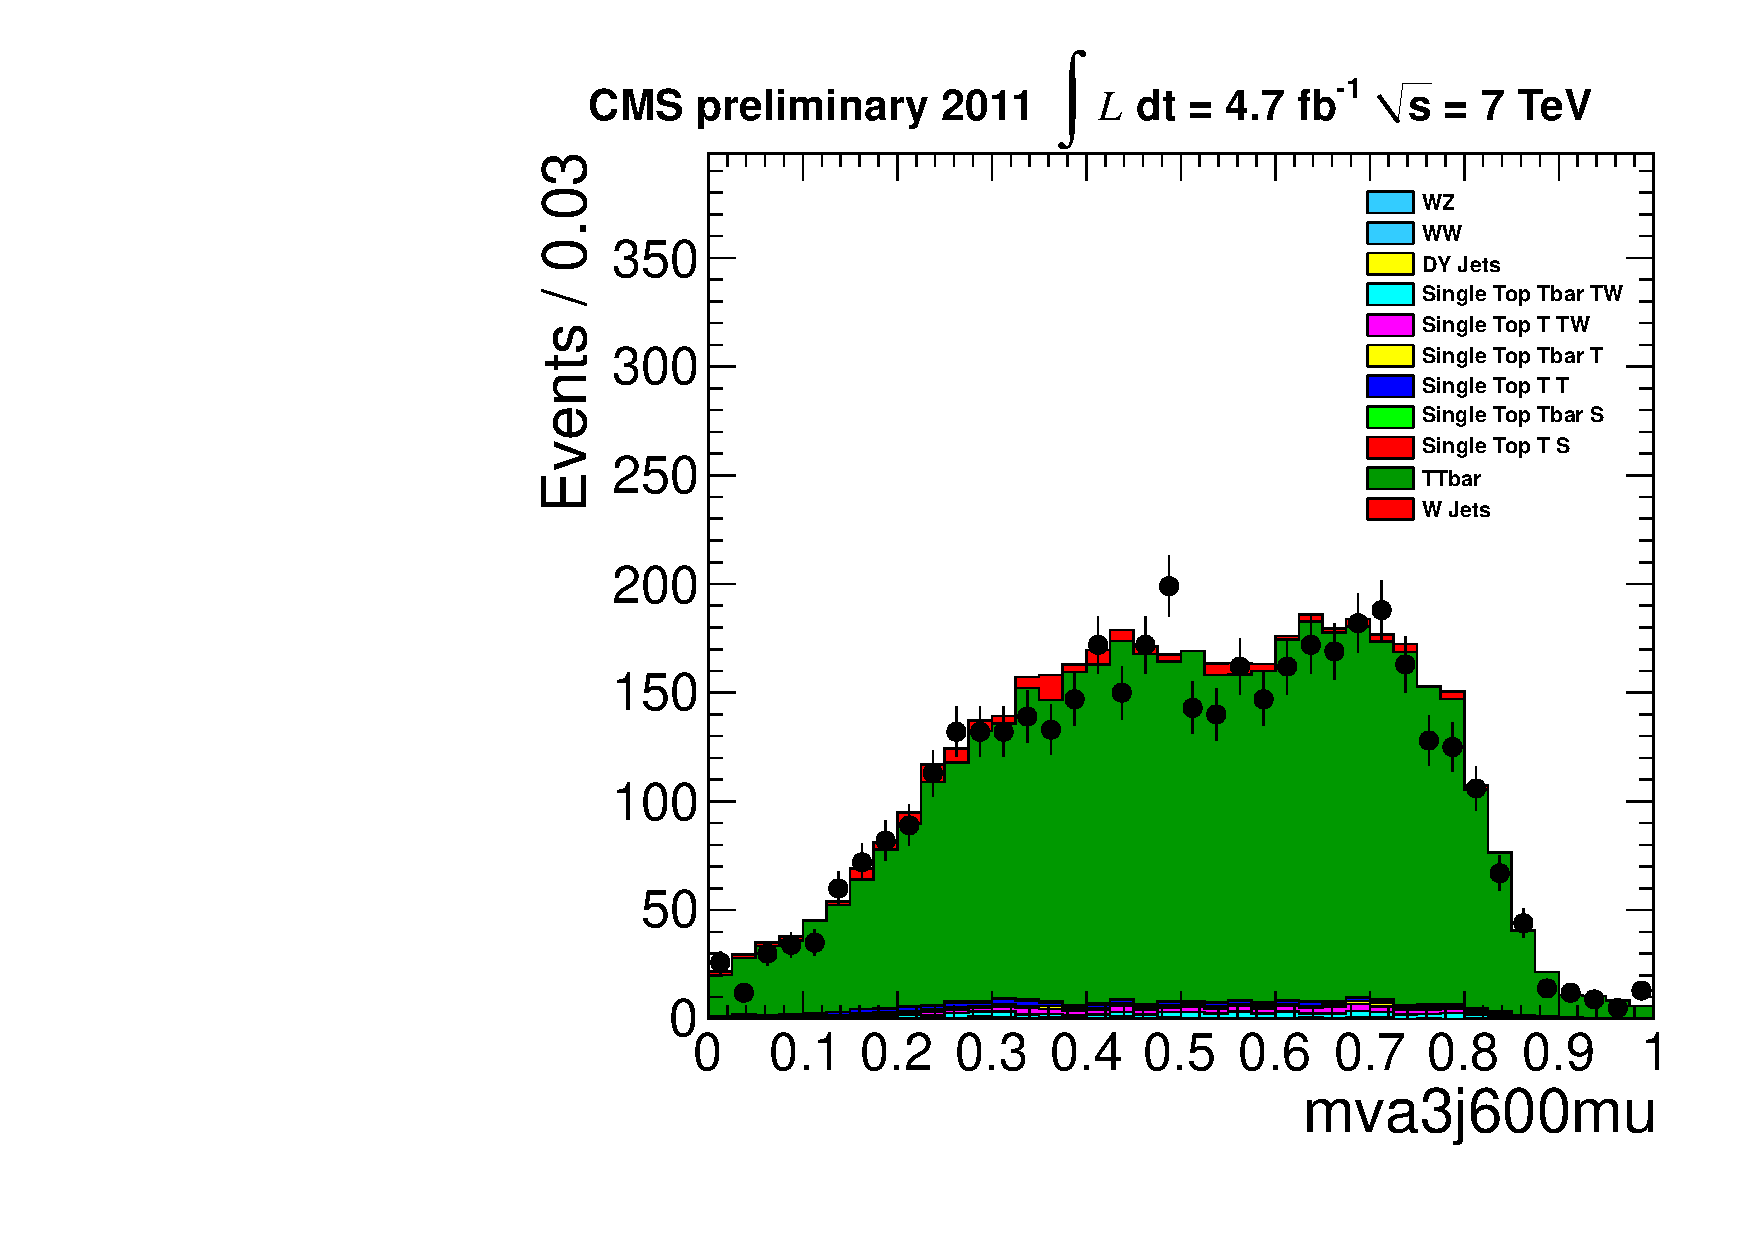
\includegraphics[width=0.49\textwidth]{figs/cl-mva3j600mu-inTTbar.pdf}
  \caption{\label{fig:mva:plots-mva3j600mu} The data-MC comparisons
    after standard event selection (left) and top pair
    selection (right) for the working point: mva3j600mu.}
\end{figure}

\clearpage
%%%%%%%%%%%%%%%%%%%%%%%%%%%%%%%%%%%%%%%%%%%%%%%%%%%%%%%%%%%%%%%%%%%%%%%%%%%%
%%%%%%%%%%%%%%%%%%% mva2j170el
\begin{figure}[!t]
  \centering
  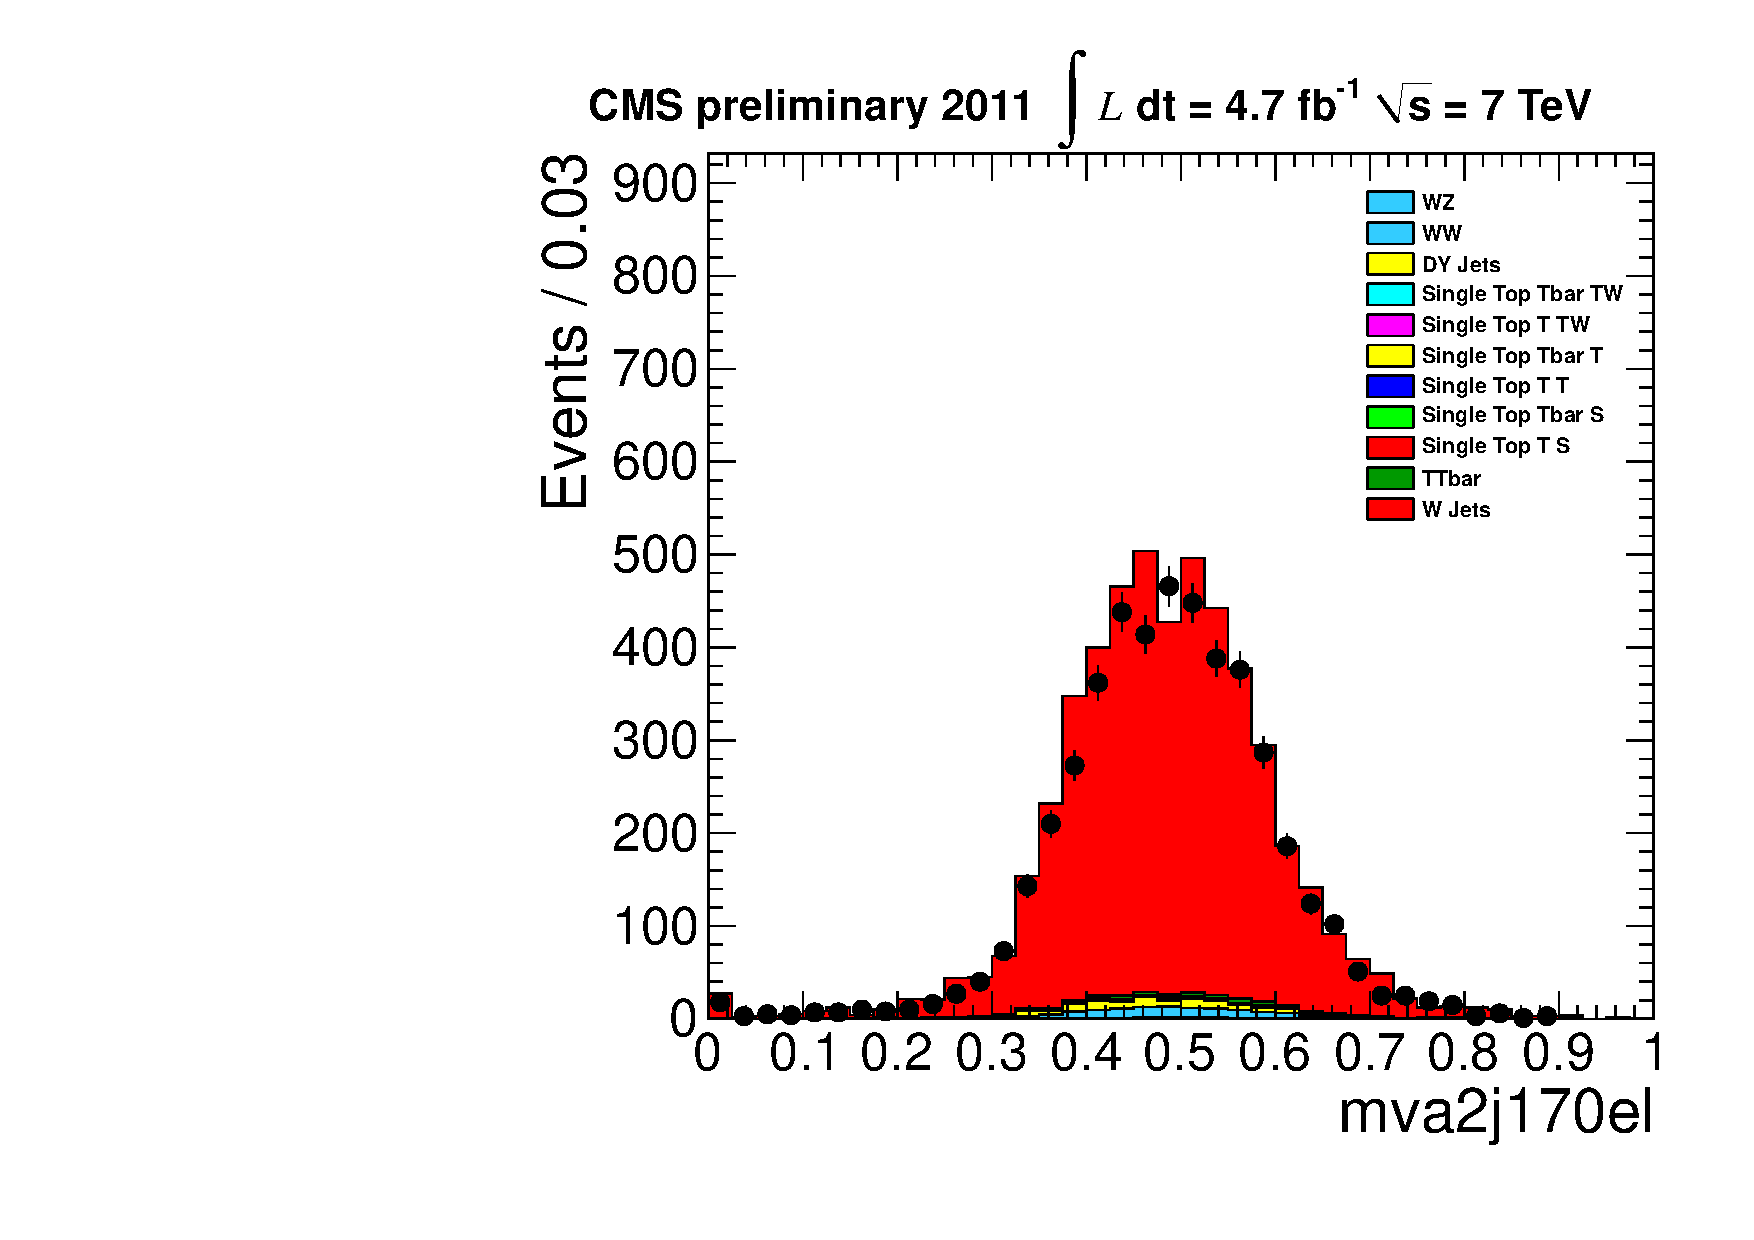
\includegraphics[width=0.49\textwidth]{figs/cl-mva2j170el-normal.pdf}
  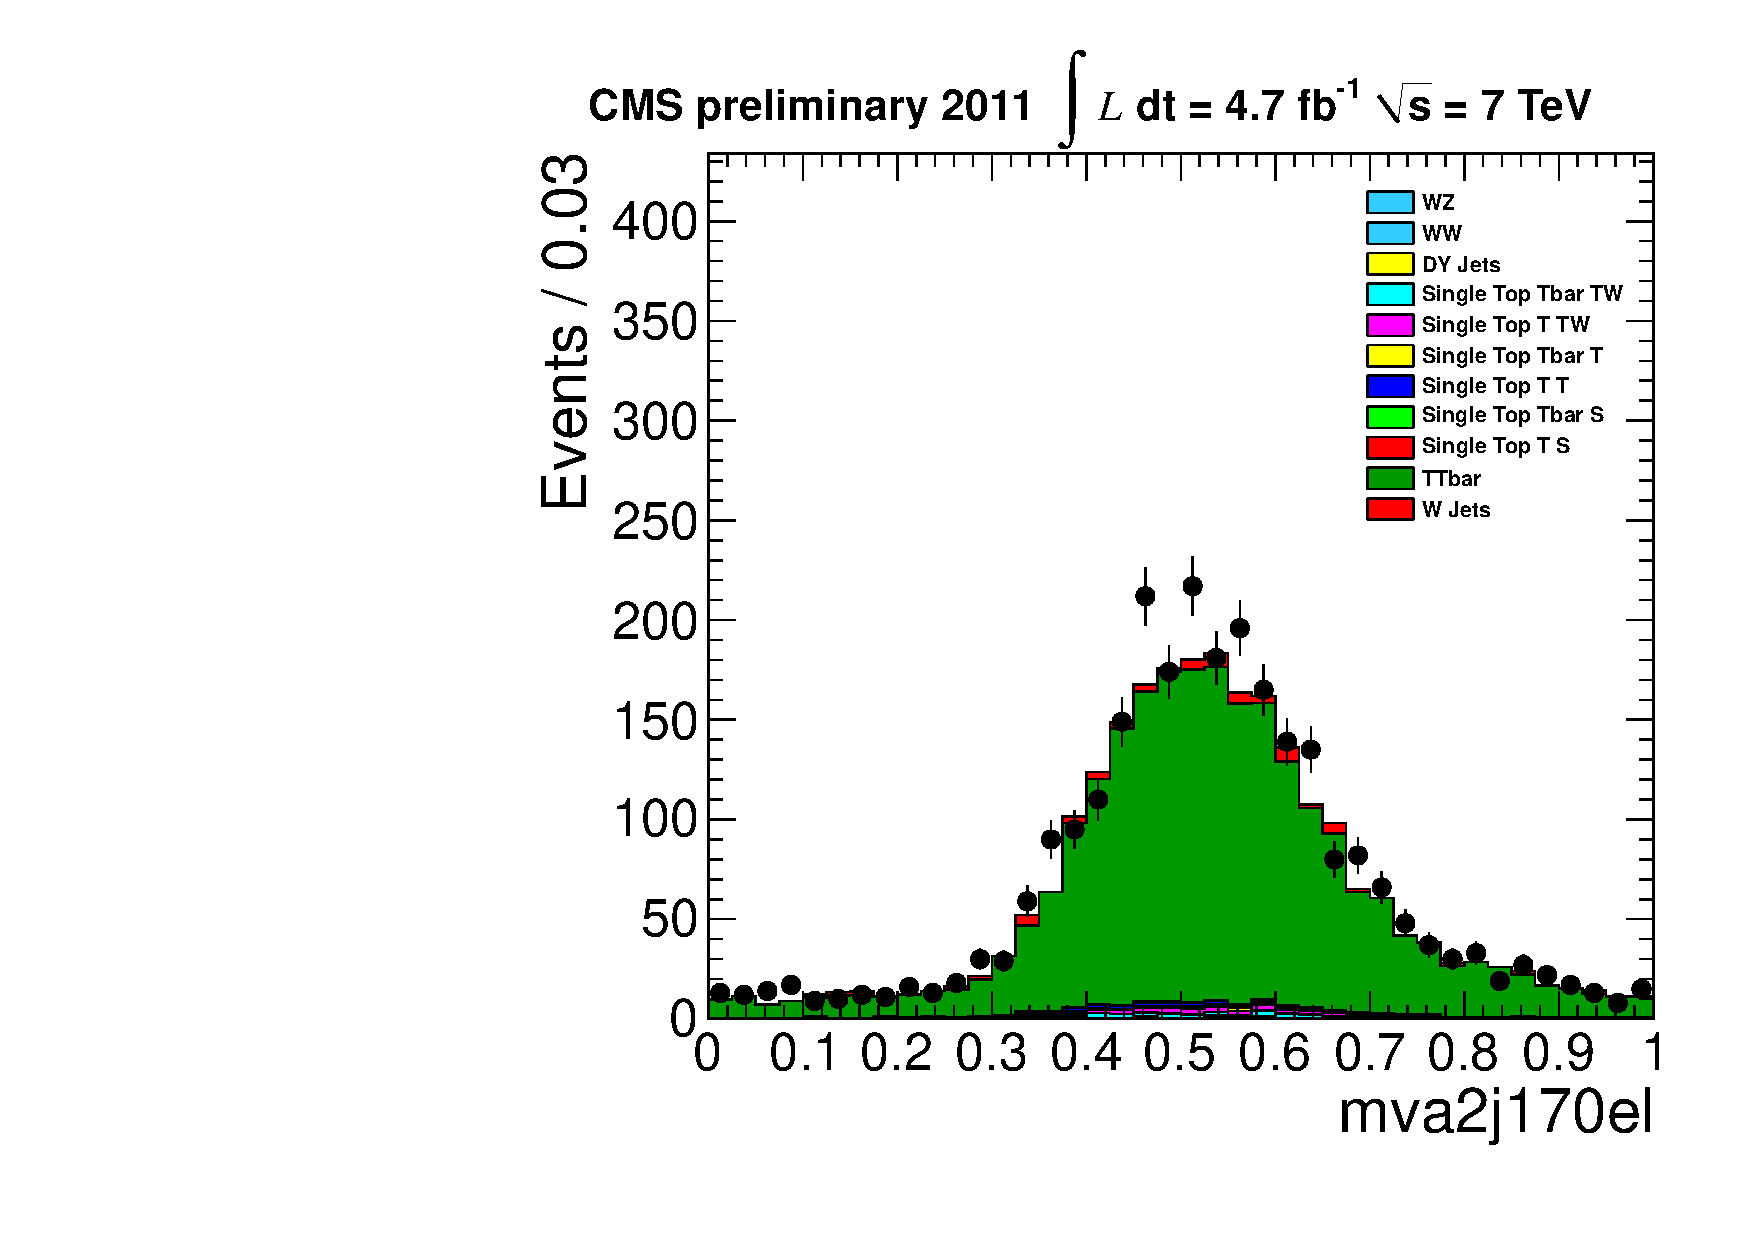
\includegraphics[width=0.49\textwidth]{figs/cl-mva2j170el-inTTbar.pdf}
  \caption{\label{fig:mva:plots-mva2j170el} The data-MC comparisons
    after standard event selection (left) and top pair
    selection (right) for the working point: mva2j170el.}
\end{figure}

%%%%%%%%%%%%%%%%%%% mva2j180el
\begin{figure}[!t]
  \centering
  \includegraphics[width=0.49\textwidth]{figs/cl-mva2j180el-normal.pdf}
  \includegraphics[width=0.49\textwidth]{figs/cl-mva2j180el-inTTbar.pdf}
  \caption{\label{fig:mva:plots-mva2j180el} The data-MC comparisons
    after standard event selection (left) and top pair
    selection (right) for the working point: mva2j180el.}
\end{figure}

%%%%%%%%%%%%%%%%%%% mva2j190el
\begin{figure}[!t]
  \centering
  \includegraphics[width=0.49\textwidth]{figs/cl-mva2j190el-normal.pdf}
  \includegraphics[width=0.49\textwidth]{figs/cl-mva2j190el-inTTbar.pdf}
  \caption{\label{fig:mva:plots-mva2j190el} The data-MC comparisons
    after standard event selection (left) and top pair
    selection (right) for the working point: mva2j190el.}
\end{figure}

%%%%%%%%%%%%%%%%%%% mva2j200el
\begin{figure}[!t]
  \centering
  \includegraphics[width=0.49\textwidth]{figs/cl-mva2j200el-normal.pdf}
  \includegraphics[width=0.49\textwidth]{figs/cl-mva2j200el-inTTbar.pdf}
  \caption{\label{fig:mva:plots-mva2j200el} The data-MC comparisons
    after standard event selection (left) and top pair
    selection (right) for the working point: mva2j200el.}
\end{figure}

%%%%%%%%%%%%%%%%%%% mva2j250el
\begin{figure}[!t]
  \centering
  \includegraphics[width=0.49\textwidth]{figs/cl-mva2j250el-normal.pdf}
  \includegraphics[width=0.49\textwidth]{figs/cl-mva2j250el-inTTbar.pdf}
  \caption{\label{fig:mva:plots-mva2j250el} The data-MC comparisons
    after standard event selection (left) and top pair
    selection (right) for the working point: mva2j250el.}
\end{figure}

%%%%%%%%%%%%%%%%%%% mva2j300el
\begin{figure}[!t]
  \centering
  \includegraphics[width=0.49\textwidth]{figs/cl-mva2j300el-normal.pdf}
  \includegraphics[width=0.49\textwidth]{figs/cl-mva2j300el-inTTbar.pdf}
  \caption{\label{fig:mva:plots-mva2j300el} The data-MC comparisons
    after standard event selection (left) and top pair
    selection (right) for the working point: mva2j300el.}
\end{figure}

%%%%%%%%%%%%%%%%%%% mva2j350el
\begin{figure}[!t]
  \centering
  \includegraphics[width=0.49\textwidth]{figs/cl-mva2j350el-normal.pdf}
  \includegraphics[width=0.49\textwidth]{figs/cl-mva2j350el-inTTbar.pdf}
  \caption{\label{fig:mva:plots-mva2j350el} The data-MC comparisons
    after standard event selection (left) and top pair
    selection (right) for the working point: mva2j350el.}
\end{figure}

%%%%%%%%%%%%%%%%%%% mva2j400el
\begin{figure}[!t]
  \centering
  \includegraphics[width=0.49\textwidth]{figs/cl-mva2j400el-normal.pdf}
  \includegraphics[width=0.49\textwidth]{figs/cl-mva2j400el-inTTbar.pdf}
  \caption{\label{fig:mva:plots-mva2j400el} The data-MC comparisons
    after standard event selection (left) and top pair
    selection (right) for the working point: mva2j400el.}
\end{figure}

%%%%%%%%%%%%%%%%%%% mva2j450el
\begin{figure}[!t]
  \centering
  \includegraphics[width=0.49\textwidth]{figs/cl-mva2j450el-normal.pdf}
  \includegraphics[width=0.49\textwidth]{figs/cl-mva2j450el-inTTbar.pdf}
  \caption{\label{fig:mva:plots-mva2j450el} The data-MC comparisons
    after standard event selection (left) and top pair
    selection (right) for the working point: mva2j450el.}
\end{figure}

%%%%%%%%%%%%%%%%%%% mva2j500el
\begin{figure}[!t]
  \centering
  \includegraphics[width=0.49\textwidth]{figs/cl-mva2j500el-normal.pdf}
  \includegraphics[width=0.49\textwidth]{figs/cl-mva2j500el-inTTbar.pdf}
  \caption{\label{fig:mva:plots-mva2j500el} The data-MC comparisons
    after standard event selection (left) and top pair
    selection (right) for the working point: mva2j500el.}
\end{figure}

%%%%%%%%%%%%%%%%%%% mva2j550el
\begin{figure}[!t]
  \centering
  \includegraphics[width=0.49\textwidth]{figs/cl-mva2j550el-normal.pdf}
  \includegraphics[width=0.49\textwidth]{figs/cl-mva2j550el-inTTbar.pdf}
  \caption{\label{fig:mva:plots-mva2j550el} The data-MC comparisons
    after standard event selection (left) and top pair
    selection (right) for the working point: mva2j550el.}
\end{figure}

%%%%%%%%%%%%%%%%%%% mva2j600el
\begin{figure}[!t]
  \centering
  \includegraphics[width=0.49\textwidth]{figs/cl-mva2j600el-normal.pdf}
  \includegraphics[width=0.49\textwidth]{figs/cl-mva2j600el-inTTbar.pdf}
  \caption{\label{fig:mva:plots-mva2j600el} The data-MC comparisons
    after standard event selection (left) and top pair
    selection (right) for the working point: mva2j600el.}
\end{figure}

\clearpage
%%%%%%%%%%%%%%%%%%%%%%%%%%%%%%%%%%%%%%%%%%%%%%%%%%%%%%%%%%%%%%%%%%%%%%%%%%%%
%%%%%%%%%%%%%%%%%%% mva3j170el
\begin{figure}[!t]
  \centering
  \includegraphics[width=0.49\textwidth]{figs/cl-mva3j170el-normal.pdf}
  \includegraphics[width=0.49\textwidth]{figs/cl-mva3j170el-inTTbar.pdf}
  \caption{\label{fig:mva:plots-mva3j170el} The data-MC comparisons
    after standard event selection (left) and top pair
    selection (right) for the working point: mva3j170el.}
\end{figure}

%%%%%%%%%%%%%%%%%%% mva3j180el
\begin{figure}[!t]
  \centering
  \includegraphics[width=0.49\textwidth]{figs/cl-mva3j180el-normal.pdf}
  \includegraphics[width=0.49\textwidth]{figs/cl-mva3j180el-inTTbar.pdf}
  \caption{\label{fig:mva:plots-mva3j180el} The data-MC comparisons
    after standard event selection (left) and top pair
    selection (right) for the working point: mva3j180el.}
\end{figure}

%%%%%%%%%%%%%%%%%%% mva3j190el
\begin{figure}[!t]
  \centering
  \includegraphics[width=0.49\textwidth]{figs/cl-mva3j190el-normal.pdf}
  \includegraphics[width=0.49\textwidth]{figs/cl-mva3j190el-inTTbar.pdf}
  \caption{\label{fig:mva:plots-mva3j190el} The data-MC comparisons
    after standard event selection (left) and top pair
    selection (right) for the working point: mva3j190el.}
\end{figure}

%%%%%%%%%%%%%%%%%%% mva3j200el
\begin{figure}[!t]
  \centering
  \includegraphics[width=0.49\textwidth]{figs/cl-mva3j200el-normal.pdf}
  \includegraphics[width=0.49\textwidth]{figs/cl-mva3j200el-inTTbar.pdf}
  \caption{\label{fig:mva:plots-mva3j200el} The data-MC comparisons
    after standard event selection (left) and top pair
    selection (right) for the working point: mva3j200el.}
\end{figure}

%%%%%%%%%%%%%%%%%%% mva3j250el
\begin{figure}[!t]
  \centering
  \includegraphics[width=0.49\textwidth]{figs/cl-mva3j250el-normal.pdf}
  \includegraphics[width=0.49\textwidth]{figs/cl-mva3j250el-inTTbar.pdf}
  \caption{\label{fig:mva:plots-mva3j250el} The data-MC comparisons
    after standard event selection (left) and top pair
    selection (right) for the working point: mva3j250el.}
\end{figure}

%%%%%%%%%%%%%%%%%%% mva3j300el
\begin{figure}[!t]
  \centering
  \includegraphics[width=0.49\textwidth]{figs/cl-mva3j300el-normal.pdf}
  \includegraphics[width=0.49\textwidth]{figs/cl-mva3j300el-inTTbar.pdf}
  \caption{\label{fig:mva:plots-mva3j300el} The data-MC comparisons
    after standard event selection (left) and top pair
    selection (right) for the working point: mva3j300el.}
\end{figure}

%%%%%%%%%%%%%%%%%%% mva3j350el
\begin{figure}[!t]
  \centering
  \includegraphics[width=0.49\textwidth]{figs/cl-mva3j350el-normal.pdf}
  \includegraphics[width=0.49\textwidth]{figs/cl-mva3j350el-inTTbar.pdf}
  \caption{\label{fig:mva:plots-mva3j350el} The data-MC comparisons
    after standard event selection (left) and top pair
    selection (right) for the working point: mva3j350el.}
\end{figure}

%%%%%%%%%%%%%%%%%%% mva3j400el
\begin{figure}[!t]
  \centering
  \includegraphics[width=0.49\textwidth]{figs/cl-mva3j400el-normal.pdf}
  \includegraphics[width=0.49\textwidth]{figs/cl-mva3j400el-inTTbar.pdf}
  \caption{\label{fig:mva:plots-mva3j400el} The data-MC comparisons
    after standard event selection (left) and top pair
    selection (right) for the working point: mva3j400el.}
\end{figure}

%%%%%%%%%%%%%%%%%%% mva3j450el
\begin{figure}[!t]
  \centering
  \includegraphics[width=0.49\textwidth]{figs/cl-mva3j450el-normal.pdf}
  \includegraphics[width=0.49\textwidth]{figs/cl-mva3j450el-inTTbar.pdf}
  \caption{\label{fig:mva:plots-mva3j450el} The data-MC comparisons
    after standard event selection (left) and top pair
    selection (right) for the working point: mva3j450el.}
\end{figure}

%%%%%%%%%%%%%%%%%%% mva3j500el
\begin{figure}[!t]
  \centering
  \includegraphics[width=0.49\textwidth]{figs/cl-mva3j500el-normal.pdf}
  \includegraphics[width=0.49\textwidth]{figs/cl-mva3j500el-inTTbar.pdf}
  \caption{\label{fig:mva:plots-mva3j500el} The data-MC comparisons
    after standard event selection (left) and top pair
    selection (right) for the working point: mva3j500el.}
\end{figure}

%%%%%%%%%%%%%%%%%%% mva3j550el
\begin{figure}[!t]
  \centering
  \includegraphics[width=0.49\textwidth]{figs/cl-mva3j550el-normal.pdf}
  \includegraphics[width=0.49\textwidth]{figs/cl-mva3j550el-inTTbar.pdf}
  \caption{\label{fig:mva:plots-mva3j550el} The data-MC comparisons
    after standard event selection (left) and top pair
    selection (right) for the working point: mva3j550el.}
\end{figure}

%%%%%%%%%%%%%%%%%%% mva3j600el
\begin{figure}[!t]
  \centering
  \includegraphics[width=0.49\textwidth]{figs/cl-mva3j600el-normal.pdf}
  \includegraphics[width=0.49\textwidth]{figs/cl-mva3j600el-inTTbar.pdf}
  \caption{\label{fig:mva:plots-mva3j600el} The data-MC comparisons
    after standard event selection (left) and top pair
    selection (right) for the working point: mva3j600el.}
\end{figure}


\clearpage
%%%%%%%%%%%%%%%%%%%%%%%%%%%%%%%%%%%%%%%%%%%%%%%%%%%%%%%%%%%%%%%%%%%%%%%%%%%%%%%%%%%%%%%%%%%%%%%
\section{MVA Output Distributions}
We use an almost pure top data control sample to study the systematics
on the Higgs signal efficiency due to the MVA output cut. These
semileptonic top events are selected by requiring exactly four jets in
the event, out of which two are b-tagged and the other two are
anti-btagged. To better understand the MVA ouput distributions, we
compare those distributions in top MC samples with Higgs signal MC
samples as shown in Fig.~\ref{fig:mva:sigvsttbar-mva2j170} to
Fig.~\ref{fig:mva:sigvsttbar-mva2j600}. 

%%%%%%%%%%%%%%%%%%% 
\begin{figure}[!t]
  \centering
  \includegraphics[width=0.49\textwidth]{figs/cl-mva2j170mu-mvaTopvsHiggs.pdf}
  \includegraphics[width=0.49\textwidth]{figs/cl-mva3j170mu-mvaTopvsHiggs.pdf}
  \includegraphics[width=0.49\textwidth]{figs/cl-mva2j170el-mvaTopvsHiggs.pdf}
  \includegraphics[width=0.49\textwidth]{figs/cl-mva3j170el-mvaTopvsHiggs.pdf}
  \caption{\label{fig:mva:sigvsttbar-mva2j170}The MVA output
    distributions in top MC sample compared with in Higgs MC
    samples for Higgs mass 170~GeV. Top-left plot is muon 2-jet category,
    top-right is muon 3-jet category, bottom-left is electron 2-jet
    category, and bottom-right is electron 3-jet category. }
\end{figure}

%%%%%%%%%%%%%%%%%%% 
\begin{figure}[!t]
  \centering
  \includegraphics[width=0.49\textwidth]{figs/cl-mva2j180mu-mvaTopvsHiggs.pdf}
  \includegraphics[width=0.49\textwidth]{figs/cl-mva3j180mu-mvaTopvsHiggs.pdf}
  \includegraphics[width=0.49\textwidth]{figs/cl-mva2j180el-mvaTopvsHiggs.pdf}
  \includegraphics[width=0.49\textwidth]{figs/cl-mva3j180el-mvaTopvsHiggs.pdf}
  \caption{\label{fig:mva:sigvsttbar-mva2j180}The MVA output
    distributions in top MC sample compared with in Higgs MC
    samples for Higgs mass 180~GeV. Top-left plot is muon 2-jet category,
    top-right is muon 3-jet category, bottom-left is electron 2-jet
    category, and bottom-right is electron 3-jet category. }
\end{figure}

%%%%%%%%%%%%%%%%%%% 
\begin{figure}[!t]
  \centering
  \includegraphics[width=0.49\textwidth]{figs/cl-mva2j190mu-mvaTopvsHiggs.pdf}
  \includegraphics[width=0.49\textwidth]{figs/cl-mva3j190mu-mvaTopvsHiggs.pdf}
  \includegraphics[width=0.49\textwidth]{figs/cl-mva2j190el-mvaTopvsHiggs.pdf}
  \includegraphics[width=0.49\textwidth]{figs/cl-mva3j190el-mvaTopvsHiggs.pdf}
  \caption{\label{fig:mva:sigvsttbar-mva2j190}The MVA output
    distributions in top MC sample compared with in Higgs MC
    samples for Higgs mass 190~GeV. Top-left plot is muon 2-jet category,
    top-right is muon 3-jet category, bottom-left is electron 2-jet
    category, and bottom-right is electron 3-jet category. }
\end{figure}

%%%%%%%%%%%%%%%%%%% 
\begin{figure}[!t]
  \centering
  \includegraphics[width=0.49\textwidth]{figs/cl-mva2j200mu-mvaTopvsHiggs.pdf}
  \includegraphics[width=0.49\textwidth]{figs/cl-mva3j200mu-mvaTopvsHiggs.pdf}
  \includegraphics[width=0.49\textwidth]{figs/cl-mva2j200el-mvaTopvsHiggs.pdf}
  \includegraphics[width=0.49\textwidth]{figs/cl-mva3j200el-mvaTopvsHiggs.pdf}
  \caption{\label{fig:mva:sigvsttbar-mva2j200}The MVA output
    distributions in top MC sample compared with in Higgs MC
    samples for Higgs mass 200~GeV. Top-left plot is muon 2-jet category,
    top-right is muon 3-jet category, bottom-left is electron 2-jet
    category, and bottom-right is electron 3-jet category. }
\end{figure}

%%%%%%%%%%%%%%%%%%% 
\begin{figure}[!t]
  \centering
  \includegraphics[width=0.49\textwidth]{figs/cl-mva2j250mu-mvaTopvsHiggs.pdf}
  \includegraphics[width=0.49\textwidth]{figs/cl-mva3j250mu-mvaTopvsHiggs.pdf}
  \includegraphics[width=0.49\textwidth]{figs/cl-mva2j250el-mvaTopvsHiggs.pdf}
  \includegraphics[width=0.49\textwidth]{figs/cl-mva3j250el-mvaTopvsHiggs.pdf}
  \caption{\label{fig:mva:sigvsttbar-mva2j250}The MVA output
    distributions in top MC sample compared with in Higgs MC
    samples for Higgs mass 250~GeV. Top-left plot is muon 2-jet category,
    top-right is muon 3-jet category, bottom-left is electron 2-jet
    category, and bottom-right is electron 3-jet category. }
\end{figure}

%%%%%%%%%%%%%%%%%%% 
\begin{figure}[!t]
  \centering
  \includegraphics[width=0.49\textwidth]{figs/cl-mva2j300mu-mvaTopvsHiggs.pdf}
  \includegraphics[width=0.49\textwidth]{figs/cl-mva3j300mu-mvaTopvsHiggs.pdf}
  \includegraphics[width=0.49\textwidth]{figs/cl-mva2j300el-mvaTopvsHiggs.pdf}
  \includegraphics[width=0.49\textwidth]{figs/cl-mva3j300el-mvaTopvsHiggs.pdf}
  \caption{\label{fig:mva:sigvsttbar-mva2j300}The MVA output
    distributions in top MC sample compared with in Higgs MC
    samples for Higgs mass 300~GeV. Top-left plot is muon 2-jet category,
    top-right is muon 3-jet category, bottom-left is electron 2-jet
    category, and bottom-right is electron 3-jet category. }
\end{figure}

%%%%%%%%%%%%%%%%%%% 
\begin{figure}[!t]
  \centering
  \includegraphics[width=0.49\textwidth]{figs/cl-mva2j350mu-mvaTopvsHiggs.pdf}
  \includegraphics[width=0.49\textwidth]{figs/cl-mva3j350mu-mvaTopvsHiggs.pdf}
  \includegraphics[width=0.49\textwidth]{figs/cl-mva2j350el-mvaTopvsHiggs.pdf}
  \includegraphics[width=0.49\textwidth]{figs/cl-mva3j350el-mvaTopvsHiggs.pdf}
  \caption{\label{fig:mva:sigvsttbar-mva2j350}The MVA output
    distributions in top MC sample compared with in Higgs MC
    samples for Higgs mass 350~GeV. Top-left plot is muon 2-jet category,
    top-right is muon 3-jet category, bottom-left is electron 2-jet
    category, and bottom-right is electron 3-jet category. }
\end{figure}

%%%%%%%%%%%%%%%%%%% 
\begin{figure}[!t]
  \centering
  \includegraphics[width=0.49\textwidth]{figs/cl-mva2j400mu-mvaTopvsHiggs.pdf}
  \includegraphics[width=0.49\textwidth]{figs/cl-mva3j400mu-mvaTopvsHiggs.pdf}
  \includegraphics[width=0.49\textwidth]{figs/cl-mva2j400el-mvaTopvsHiggs.pdf}
  \includegraphics[width=0.49\textwidth]{figs/cl-mva3j400el-mvaTopvsHiggs.pdf}
  \caption{\label{fig:mva:sigvsttbar-mva2j400}The MVA output
    distributions in top MC sample compared with in Higgs MC
    samples for Higgs mass 400~GeV. Top-left plot is muon 2-jet category,
    top-right is muon 3-jet category, bottom-left is electron 2-jet
    category, and bottom-right is electron 3-jet category. }
\end{figure}

%%%%%%%%%%%%%%%%%%% 
\begin{figure}[!t]
  \centering
  \includegraphics[width=0.49\textwidth]{figs/cl-mva2j450mu-mvaTopvsHiggs.pdf}
  \includegraphics[width=0.49\textwidth]{figs/cl-mva3j450mu-mvaTopvsHiggs.pdf}
  \includegraphics[width=0.49\textwidth]{figs/cl-mva2j450el-mvaTopvsHiggs.pdf}
  \includegraphics[width=0.49\textwidth]{figs/cl-mva3j450el-mvaTopvsHiggs.pdf}
  \caption{\label{fig:mva:sigvsttbar-mva2j450}The MVA output
    distributions in top MC sample compared with in Higgs MC
    samples for Higgs mass 450~GeV. Top-left plot is muon 2-jet category,
    top-right is muon 3-jet category, bottom-left is electron 2-jet
    category, and bottom-right is electron 3-jet category. }
\end{figure}

%%%%%%%%%%%%%%%%%%% 
\begin{figure}[!t]
  \centering
  \includegraphics[width=0.49\textwidth]{figs/cl-mva2j500mu-mvaTopvsHiggs.pdf}
  \includegraphics[width=0.49\textwidth]{figs/cl-mva3j500mu-mvaTopvsHiggs.pdf}
  \includegraphics[width=0.49\textwidth]{figs/cl-mva2j500el-mvaTopvsHiggs.pdf}
  \includegraphics[width=0.49\textwidth]{figs/cl-mva3j500el-mvaTopvsHiggs.pdf}
  \caption{\label{fig:mva:sigvsttbar-mva2j500}The MVA output
    distributions in top MC sample compared with in Higgs MC
    samples for Higgs mass 500~GeV. Top-left plot is muon 2-jet category,
    top-right is muon 3-jet category, bottom-left is electron 2-jet
    category, and bottom-right is electron 3-jet category. }
\end{figure}

%%%%%%%%%%%%%%%%%%% 
\begin{figure}[!t]
  \centering
  \includegraphics[width=0.49\textwidth]{figs/cl-mva2j550mu-mvaTopvsHiggs.pdf}
  \includegraphics[width=0.49\textwidth]{figs/cl-mva3j550mu-mvaTopvsHiggs.pdf}
  \includegraphics[width=0.49\textwidth]{figs/cl-mva2j550el-mvaTopvsHiggs.pdf}
  \includegraphics[width=0.49\textwidth]{figs/cl-mva3j550el-mvaTopvsHiggs.pdf}
  \caption{\label{fig:mva:sigvsttbar-mva2j550}The MVA output
    distributions in top MC sample compared with in Higgs MC
    samples for Higgs mass 550~GeV. Top-left plot is muon 2-jet category,
    top-right is muon 3-jet category, bottom-left is electron 2-jet
    category, and bottom-right is electron 3-jet category. }
\end{figure}

%%%%%%%%%%%%%%%%%%% 
\begin{figure}[!t]
  \centering
  \includegraphics[width=0.49\textwidth]{figs/cl-mva2j600mu-mvaTopvsHiggs.pdf}
  \includegraphics[width=0.49\textwidth]{figs/cl-mva3j600mu-mvaTopvsHiggs.pdf}
  \includegraphics[width=0.49\textwidth]{figs/cl-mva2j600el-mvaTopvsHiggs.pdf}
  \includegraphics[width=0.49\textwidth]{figs/cl-mva3j600el-mvaTopvsHiggs.pdf}
  \caption{\label{fig:mva:sigvsttbar-mva2j600}The MVA output
    distributions in top MC sample compared with in Higgs MC
    samples for Higgs mass 600~GeV. Top-left plot is muon 2-jet category,
    top-right is muon 3-jet category, bottom-left is electron 2-jet
    category, and bottom-right is electron 3-jet category. }
\end{figure}
